% Options for packages loaded elsewhere
\PassOptionsToPackage{unicode}{hyperref}
\PassOptionsToPackage{hyphens}{url}
\PassOptionsToPackage{dvipsnames,svgnames*,x11names*}{xcolor}
%
\documentclass[
]{krantz}
\usepackage{pdfpages}
\usepackage{lmodern}
\usepackage{amssymb,amsmath}
\usepackage{ifxetex,ifluatex}
\ifnum 0\ifxetex 1\fi\ifluatex 1\fi=0 % if pdftex
  \usepackage[T1]{fontenc}
  \usepackage[utf8]{inputenc}
  \usepackage{textcomp} % provide euro and other symbols
\else % if luatex or xetex
  \usepackage{unicode-math}
  \defaultfontfeatures{Scale=MatchLowercase}
  \defaultfontfeatures[\rmfamily]{Ligatures=TeX,Scale=1}
  \setmonofont[Scale=0.7]{Source Code Pro}
\fi
% Use upquote if available, for straight quotes in verbatim environments
\IfFileExists{upquote.sty}{\usepackage{upquote}}{}
\IfFileExists{microtype.sty}{% use microtype if available
  \usepackage[]{microtype}
  \UseMicrotypeSet[protrusion]{basicmath} % disable protrusion for tt fonts
}{}
\makeatletter
\@ifundefined{KOMAClassName}{% if non-KOMA class
  \IfFileExists{parskip.sty}{%
    \usepackage{parskip}
  }{% else
    \setlength{\parindent}{0pt}
    \setlength{\parskip}{6pt plus 2pt minus 1pt}}
}{% if KOMA class
  \KOMAoptions{parskip=half}}
\makeatother
\usepackage{xcolor}
\IfFileExists{xurl.sty}{\usepackage{xurl}}{} % add URL line breaks if available
\IfFileExists{bookmark.sty}{\usepackage{bookmark}}{\usepackage{hyperref}}
\hypersetup{
  pdftitle={Nova Scotia Congenital Anomalies Surveillance System},
  pdfauthor={Reproductive Care Program of Nova Scotia},
  colorlinks=true,
  linkcolor=Maroon,
  filecolor=Maroon,
  citecolor=Blue,
  urlcolor=Blue,
  pdfcreator={LaTeX via pandoc}}
\urlstyle{same} % disable monospaced font for URLs
\usepackage{longtable,booktabs}
% Correct order of tables after \paragraph or \subparagraph
\usepackage{etoolbox}
\makeatletter
\patchcmd\longtable{\par}{\if@noskipsec\mbox{}\fi\par}{}{}
\makeatother
% Allow footnotes in longtable head/foot
\IfFileExists{footnotehyper.sty}{\usepackage{footnotehyper}}{\usepackage{footnote}}
\makesavenoteenv{longtable}
\usepackage{graphicx}
\makeatletter
\def\maxwidth{\ifdim\Gin@nat@width>\linewidth\linewidth\else\Gin@nat@width\fi}
\def\maxheight{\ifdim\Gin@nat@height>\textheight\textheight\else\Gin@nat@height\fi}
\makeatother
% Scale images if necessary, so that they will not overflow the page
% margins by default, and it is still possible to overwrite the defaults
% using explicit options in \includegraphics[width, height, ...]{}
\setkeys{Gin}{width=\maxwidth,height=\maxheight,keepaspectratio}
% Set default figure placement to htbp
\makeatletter
\def\fps@figure{htbp}
\makeatother
\setlength{\emergencystretch}{3em} % prevent overfull lines
\providecommand{\tightlist}{%
  \setlength{\itemsep}{0pt}\setlength{\parskip}{0pt}}
\setcounter{secnumdepth}{5}
\usepackage{pdfpages}
\frontmatter
\usepackage{booktabs}
\usepackage{longtable}
\usepackage{array}
\usepackage{multirow}
\usepackage{wrapfig}
\usepackage{float}
\usepackage{colortbl}
\usepackage{pdflscape}
\usepackage{tabu}
\usepackage{threeparttable}
\usepackage{threeparttablex}
\usepackage[normalem]{ulem}
\usepackage{makecell}
\usepackage{xcolor}

\title{Nova Scotia Congenital Anomalies Surveillance System}
\usepackage{etoolbox}
\makeatletter
\providecommand{\subtitle}[1]{% add subtitle to \maketitle
  \apptocmd{\@title}{\par {\large #1 \par}}{}{}
}
\makeatother
\subtitle{First Report, 1987-2022}
\author{Reproductive Care Program of Nova Scotia}
\date{2023-05-18}

\begin{document}
\pagestyle{empty}
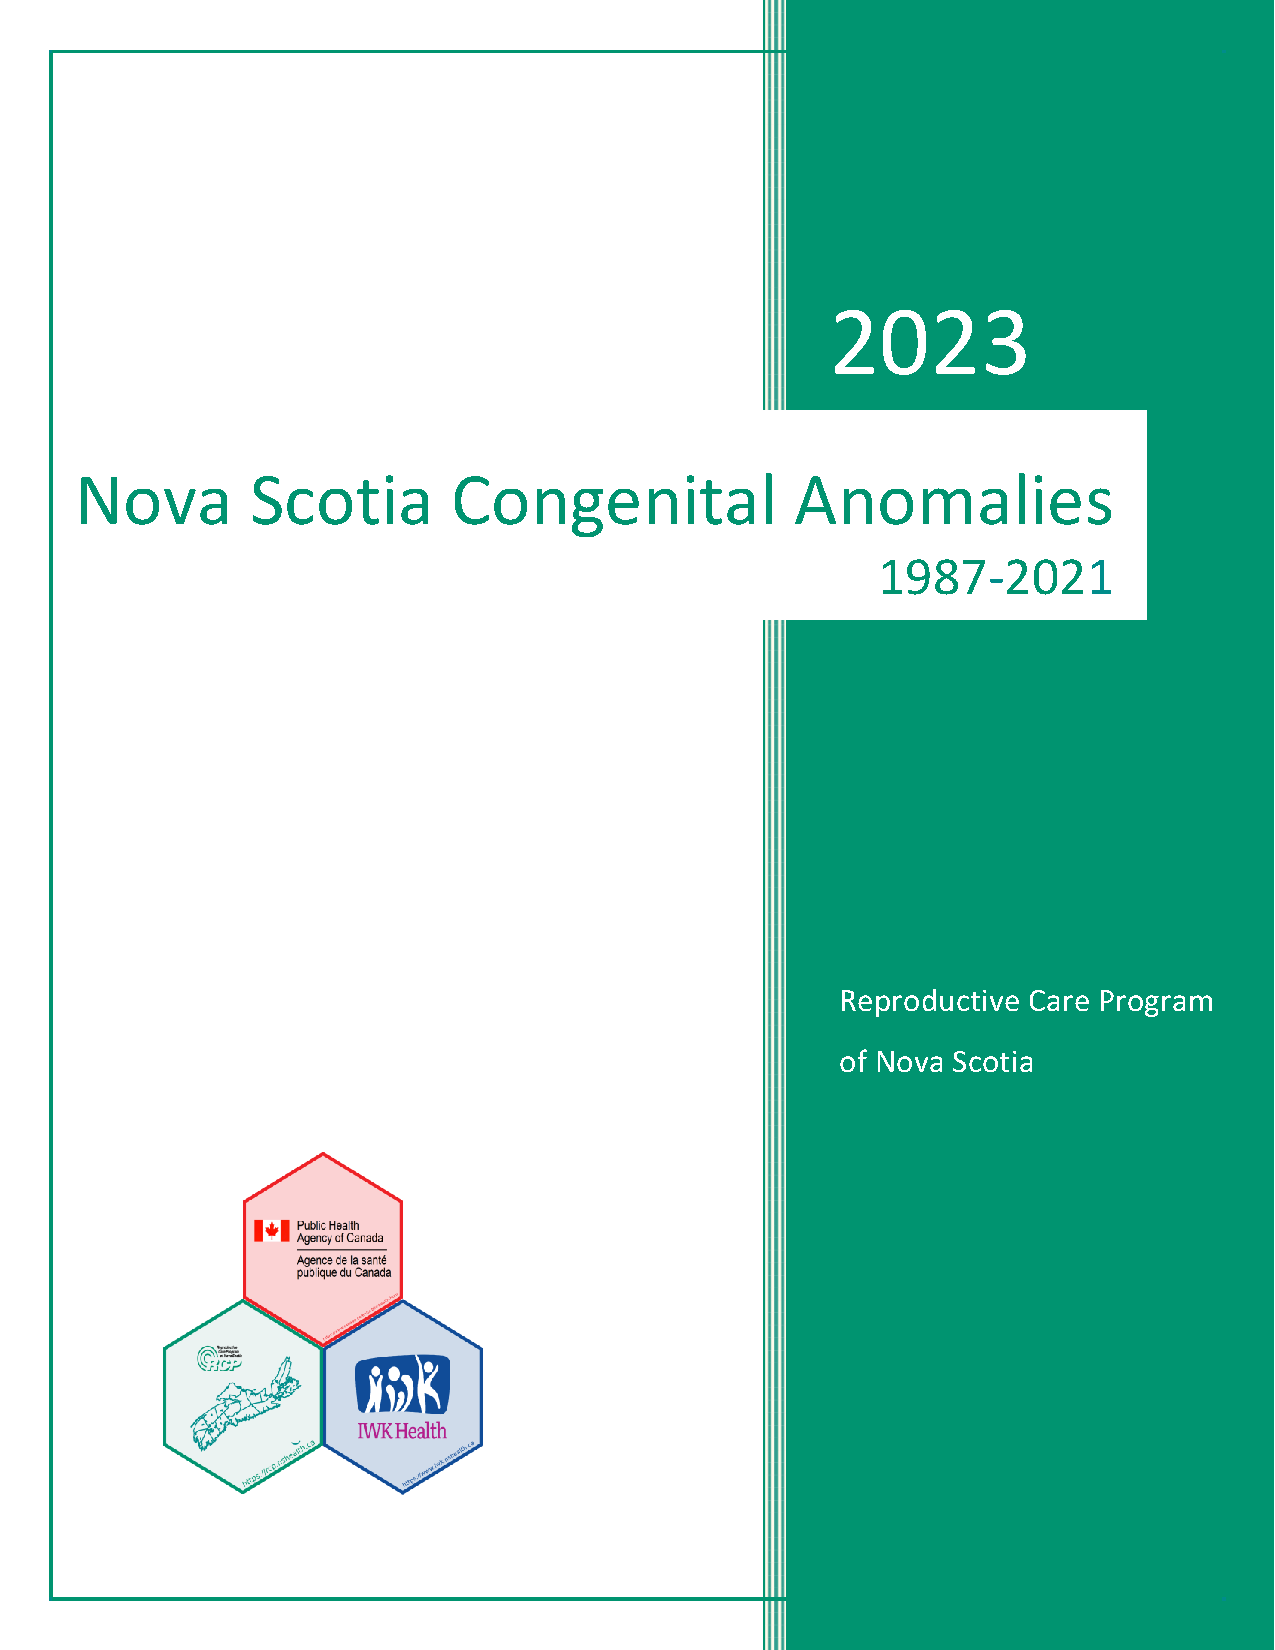
\includepdf{images/cover4.pdf}
\setcounter{page}{1}
\maketitle
\thispagestyle{empty}
\newpage


{
\hypersetup{linkcolor=}
\setcounter{tocdepth}{3}
\tableofcontents
\newpage
}


\hypertarget{background}{%
\chapter*{Background}\label{background}}


Gaps exist in the nation's capacity to conduct surveillance for congenital anomalies. In \(2002\), the Canadian Congenital Anomalies Surveillance Network (CCASN) was established

\begin{quote}
To support the development and maintenance of high quality population-based surveillance systems of congenital anomalies that will provide information to improve the health of Canadian children and their families.\footnote{Public Health Agency of Canada. What is Canadian Congenital Anomalies Surveillance Network (CCASN)}(\url{http://www.phac-aspc.gc.ca/ccasn-rcsac/index-eng.php})
\end{quote}

The CCASN produced a series of documents regarding the establishment of provincial/territorial surveillance systems for congenital anomalies\footnote{Canadian Congenital Anomalies Surveillance Network. Recommendations concerning the establishment of congenital anomalies surveillance in Canadian jurisdictions.}(), coding of congenital anomalies\footnote{Canadian Congenital Anomalies Surveillance Network. Coding of fetal anomalies.}(\url{https://health-infobase.canada.ca/congenital-anomalies/}), and delineating data elements required for minimal and enhanced surveillance for congenital anomalies\footnote{Canadian Congenital Anomalies Surveillance Network. Recommended data variables for congenital anomalies surveillance in Canadian provinces \& territories.}(\url{https://www.phac-aspc.gc.ca/ccasn-rcsac/sac-cas/pdf/cas-eng.pdf}).

In Nova Scotia, data regarding congenital anomalies diagnosed at birth or during the birth admission have been collected since \(1987\) in the Nova Scotia Atlee Perinatal Database (NSAPD) managed by the Reproductive Care Program of Nova Scotia (RCP). The NSAPD collects data about all live born infants and stillbirths for all fetuses delivered \(\ge 20\) weeks gestation, or \(\ge 500\) grams, or live born and all co-multiples of the aforementioned; the NSAPD also captures information about the mothers of the infants/fetuses mentioned above. The NSAPD does not capture data for congenital anomaly cases identified during admissions that occur after \(28\) days of age. The NSAPD also does not capture data for pregnancies ending in termination.

Since \(1992\), data regarding congenital anomalies diagnosed antenatally, or postnatally up to the time of discharge from the IWK Health Centre, or on the basis of an autopsy have been captured through the Fetal Anomaly Database (FADB) housed at the Division of Maternal and Fetal Medicine, IWK Health Centre. The IWK is the only obstetrics/paediatric tertiary care centre in the Maritimes; as such, the FADB captures most congenital anomaly cases in Nova Scotia resulting in live births, still births, and terminations. The FADB does not capture congenital anomaly cases diagnosed after the birth admission, many of which are present in other data sources within the province. The FADB also uses an in-house coding system to classify anomalies, a practice that predates the CCASN recommendation to use the Royal College of Paediatrics and Child Health codes (adapted from the \href{https://www.google.ca/url?sa=t\&rct=j\&q=\&esrc=s\&source=web\&cd=\&ved=2ahUKEwi9rdLH6pT7AhU2kIkEHUtrDgIQFnoECBgQAQ\&url=https\%3A\%2F\%2Fapps.who.int\%2Firis\%2Fbitstream\%2Fhandle\%2F10665\%2F246208\%2F9789241549165-V1-eng.pdf\&usg=AOvVaw1TYOJuoOf2vUt7kCVsCziR}{International Statistical Classification of Diseases and Related Health Problems, 10th Revision -- ICD-10}).

\hypertarget{scan-ns-activity-and-report-summary}{%
\chapter*{SCAN-NS Activity and Report Summary}\label{scan-ns-activity-and-report-summary}}


\begin{enumerate}
\def\labelenumi{\arabic{enumi}.}
\item
  This is the first provincial report on the prevalence of congenital anomalies in Nova Scotia generated by the Surveillance of Congenital Anomalies in Nova Scotia project.
\item
  The International Classification of Diseases - \(10^{th}\) Edition (ICD-10-CA) has been adopted by the IWK Health Centre as the reporting classification system and SCA-NS uses the Royal College of Paediatrics and Child Health adaptation of ICD-10 as well. The anomalies outlined in this report reflect the ``sentinel anomalies list'' adopted by the Nova Scotia Congenital Anomaly Advisory Group. Other anomaly data is collected and available upon request.
\item
  Nova Scotia continues to participate in the Canadian Congenital Anomalies Surveillance System (CCASS), administered by the Maternal and Infant Health Section of PHAC.
\item
  The numerator data include live births, stillbirths, and also fetal losses \(< 20\) weeks gestation with congenital anomalies. Denominator data include live births and stillbirths only. By including fetal losses in the numerator, the reported rates should be more representative of true congenital anomaly rates. Fetal losses have been ascertained since \(1992\).
\item
  Data provided in this report is a compilation of several data Nova Scotia databases.
\end{enumerate}

\begin{itemize}
\tightlist
\item
  Nova Scotia Atlee Perinatal Database (NSAPD).
\item
  Fetal Anomaly Database (FADB).
\item
  Canadian Institute for Health Information Discharge Abstract Database.
\item
  Vital Statistics Database; Service Nova Scotia.
\item
  Medical Services Insurance (MSI) Claims.
\end{itemize}

\begin{enumerate}
\def\labelenumi{\arabic{enumi}.}
\setcounter{enumi}{5}
\item
  Data within SCA-NS includes the years \(1992-2021\) however data for additional years are available for specific inquiries.
\item
  Congenital anomaly rates have remained relatively stable over the years with fluctuations occurring on a year to year basis and among specific anomalies.
\end{enumerate}

\hypertarget{introduction}{%
\chapter*{Introduction}\label{introduction}}


The purpose of SCA-NS is to improve Congenital Anomaly case ascertainment, cluster detection, local and national data comparison and reporting capability. Program objectives

\begin{itemize}
\tightlist
\item
  Provide baseline data on occurrence.
\item
  Identify populations at increased risk.
\item
  Monitor changes in occurrence.
\item
  Investigate clusters.
\item
  Refer affected children to services.
\item
  Evaluate prevention programs.
\item
  Create research opportunities.
\end{itemize}

SCA-NS includes all Nova Scotia residents, with ascertainment from other Maritime Provinces for those cases where the mother delivered elsewhere. Information on cases includes the prenatal period up to one year of age including live births, stillbirths and terminations of pregnancies in which a fetal anomaly has been detected.

\mainmatter

\hypertarget{chapter1}{%
\chapter{Methodology}\label{chapter1}}

\hypertarget{section11}{%
\section{Case Definitions}\label{section11}}

A congenital anomaly is an abnormality that is present at birth, even if not diagnosed until months or years later. Most congenital anomalies are present long before the time of birth, some in the embryonic period (up to the end of the seventh week of gestation) and others in the fetal period (eighth week to term). The term ``anomaly'' covers all the major classes of abnormalities of development, of which there are four major categories as follows:

\begin{itemize}
\item
  \textbf{Malformation -} a morphologic defect of an organ, part of an organ or a larger region of the body resulting from an intrinsically abnormal developmental process (e.g., spina bifida, cleft lip and palate).
\item
  \textbf{Deformation -} an abnormal form, shape or position of a part of the body caused by mechanical forces (e.g., extrinsic force such as intrauterine constraint causing some forms of clubfoot).
\item
  \textbf{Disruption -} a morphologic defect of an organ, part of an organ or a larger region of the body resulting from the extrinsic breakdown of, or an interference with, an originally normal developmental process (e.g., an infection such as rubella or a teratogen such as thalidomide).
\item
  \textbf{Dysplasia -} the abnormal organization of cells into tissues and its morphologic result (e.g., Marfan Syndrome, osteogenesis imperfecta).
\end{itemize}

Other definitions related to pregnancy outcomes for the purposes of this report are as follows:

\begin{itemize}
\item
  \textbf{Live birth -} a complete expulsion or extraction from the mother, irrespective of the duration of the pregnancy, of a fetus in which, after expulsion or extraction, there is breathing, beating of the heart, pulsation of the umbilical cord or definite movement of voluntary muscle (Alberta Vital Statistics Annual review, 2000).
\item
  \textbf{Stillbirth -} a complete expulsion or extraction from the mother, after at \(20\) weeks of pregnancy or more or after attaining a weight of 500 grams or more, of a fetus in which, after the expulsion or extraction, there is no breathing, beating of the heart, pulsation of the umbilical cord or unmistakable movement of voluntary muscle (Alberta Vital Statistics Annual review\footnote{ \href{https://open.alberta.ca/publications/1485-3809}{Alberta Vital Statistics Annual review}}).
\item
  \textbf{Gestation -} completed weeks of pregnancy at delivery.
\item
  \textbf{Preterm birth (a.k.a premature) -} a birth before \(37\) weeks of gestation (\(< 37\) weeks).
\item
  \textbf{Termination of Pregnancy (ToP) -} for our purposes, includes any pregnancy loss before 20 weeks gestation (\(< 20\) weeks). Most cases are therapeutic terminations for congenital anomalies but spontaneous abortions or intrauterine fetal deaths with fetal anomalies could also be included.
\end{itemize}

Anomaly definitions are based, for the most part, on those provided by the International Clearinghouse for Birth Defects Surveillance and Research (ICBDSR) and National Birth Defects Prevention Network (NBDPN).

\hypertarget{section12}{%
\section{Case Acertainment}\label{section12}}

An infant can be ascertained at any time up to the first birthday. Multiple ascertainment of the same infant can occur and is encouraged, as this frequently improves the quality and reliability of the data.

As several malformations may occur in the same infant, it is advantageous to allow each to be reported so that groups of associated malformations may be studied. This, however, leads to difficulties since the final tabulations may be reported as total malformations (anomaly rates) or as the total number of malformed infants (case rates). The tables in {[}Appendix A3{]} report anomaly rates, which in most cases are similar to case rates (e.g.~cleft palate, hypospadias, microcephaly. Whereas with limb anomalies, there can be multiple different limb anomalies in the same infant.

SCA-NS obtains information about infants with congenital anomalies from a variety of independent sources. Acquisition of additional reporting agencies is always a priority since the use of multiple sources of information improves not only the ease but also completeness of ascertainment as well as for verification of the diagnostic data.

\hypertarget{section13}{%
\section{Quality Control Measures and Data Linkage}\label{section13}}

Data quality is ensured through both a coded linking process and by manual chart audits of unmatched anomaly records. The first step in data quality control involves the linking of disparate fetal/infant records between databases. Linking is based on the matching of several unique variables in each record.

\begin{itemize}
\item
  If two records ``pass'': this variable matching process, the records are considered link and therefore report anomalies on the same fetus/infant. This allows SCA-NS to create a record that reports anomalies from several databases for the same fetus/infant.
\item
  If there are records that ``fail'' the automated matching process they are reviewed manually to determine if that information was only found in one data source or if information was entered incorrectly.
\end{itemize}

\hypertarget{section14}{%
\section{Confidentiality and Release of Data}\label{section14}}

\hypertarget{authority-for-the-collection-use-and-disclosure-of-personal-information}{%
\subsection*{Authority for the Collection, Use, and Disclosure of Personal Information}\label{authority-for-the-collection-use-and-disclosure-of-personal-information}}


In Nova Scotia, personal health information is protected by legislation, policies, and professional codes of ethics of healthcare providers. SCA-NS will follow the provisions outlined in the IWK's Privacy of Personal Health Information policy and the RCP Privacy Policy\footnote{ \href{http://rcp.nshealth.ca/about/privacy-personal-information}{RCP Privacy Policy}} and the Data Access for Research and Planning Policy and Procedures\footnote{ \href{https://rcp.nshealth.ca/sites/default/files/atlee-database/nsapd_data_access_policy_nov2007.pdf}{Data Access for Research and Planning Policy and Procedures}}

\hypertarget{data-requests}{%
\subsection*{Data Requests}\label{data-requests}}


Data requests will be reviewed by a sub-committee of the Joint Perinatal Epidemiology Research Unit-Population Health Research Unit-RCP Data Access Committee (JDAC). Clinical and technical staff will participate, as will representatives from all stakeholders currently involved in providing data, i.e.~Maternal-Fetal Medicine, BIAP, both with a privacy and a technical representative, and other groups such as Cardiology, as the database develops. Disclosure for research purposes also requires approval by a recognized Research Ethics Board and, if approved, a Data Use Agreement. SCA-NS will only consider disclosing individual level data (with or without personal identifiers) following a technical review and approval from a specially-constituted committee.

\hypertarget{limitations-of-data-and-analysis}{%
\subsection*{Limitations of Data and Analysis}\label{limitations-of-data-and-analysis}}


One of the major limitations of any surveillance system is that on its own, the information provided does not allow etiology to be determined. If trends indicate a potential problem, then separate investigative studies need to be done. However, with appropriate approvals in place, it would be possible to conduct linkage studies with other data sources to explore potential causes of specific birth defects. SCA-NS data are collected passively from a variety of sources and the completeness and accuracy of data are largely dependent on reporting and coding of several different organizations. SCA-NS reviews anomalies that have been entered into the database on a regular basis. Detailed studies of some individual anomalies or anomaly groups aid in the assessment and maintenance of the data quality. With intensive review, some cases might be reassigned, re-coded or discarded altogether from the database. This continuing review might explain some discrepancies in the data from earlier reports.

\hypertarget{epidemiological-and-statistical-measures}{%
\subsection*{Epidemiological and Statistical Measures}\label{epidemiological-and-statistical-measures}}


\begin{itemize}
\tightlist
\item
  Unless otherwise stated, all the formulas used to compute prevalence and confidence intervals are calculated following the \href{http://www.nbdpn.org/docs/Ch_8_Statistics6-04_2016DEC14.pdf}{National Birth Defects Prevention Network (NBDPN) guidelines, chapter 8}:
\end{itemize}

\begin{quote}
\[
\substack{\text{Prevalence} \\ \\ \text{at birth}} = 1,000 \times \dfrac{\text{Number of cases with birth defect A in an area and time period}}{\text{Number of live births and stillbirths in that area and time period}}
\]
\end{quote}

\begin{itemize}
\tightlist
\item
  \textbf{Pregnancy outcomes included -} the cases in the \textbf{numerator} are derived from all pregnancy outcomes collected by the program and may include:

  \begin{itemize}
  \tightlist
  \item
    Live births.
  \item
    Stillbirths.
  \item
    Termination of pregnancy (ToP): all fetal losses \(< 20\) weeks gestation with congenital anomalies.
  \end{itemize}
\end{itemize}

For the \textbf{denominator}, we use the total number of live births and stillbirths in the same area and time period from which the cases were ascertained.

\hypertarget{confidence-intervals}{%
\subsubsection*{Confidence intervals}\label{confidence-intervals}}


(\(95\%\)) confidence intervals are also included because the rate obtained is actually only a point estimate of the unknown, true population rate. The confidence interval provides information about the precision of the estimate. Thus, the confidence intervals are an estimated range of values within which there is a \(95\%\) probability that the true population rate will fall.

\begin{itemize}
\tightlist
\item
  \textbf{\emph{For a prevalence based on a small number of cases -}} For small numbers of cases (arbitrarily defined here as \(< 30\) cases), we use the Poisson distribution since birth defects are considered to be rare events. The easiest way to use the Poisson distribution is to refer to a table that provides the upper and lower \(95\%\) confidence limits for an observed number of cases. For that, we make use of the relationship between the Poisson and chi-square distribution functions. If \(X\) is a single observation from a Poisson distribution with mean \(\mu\). Then the ``exact'' \(95\%\) confidence limits for \(\mu\) are given by
\end{itemize}

\begin{quote}
\[
\small{
\left[\dfrac{qchisq\left(0.025, 2X\right)}{2}; \dfrac{qchisq\left(0.975, 2(X+1)\right)}{2}\right]},
\]
\end{quote}

where \(qchisq()\) is the quantile function for the chi-squared \(\left(\chi^{2}\right)\) distribution with \(2X\), and \(2(X+1)\) degrees of freedom. These limits can be computed using any statistical software or taken from a chi-square table (reproduced below for up to \(5\) cases).

\begin{table}

\caption{\label{tab:pois1}}
\centering
\begin{tabular}[t]{rrr}
\toprule
Number of Cases & Lower Bound & Upper Bound\\
\midrule
0 & 0.000 & 3.689\\
1 & 0.025 & 5.572\\
2 & 0.242 & 7.225\\
3 & 0.619 & 8.767\\
4 & 1.090 & 10.242\\
\addlinespace
5 & 1.623 & 11.668\\
\bottomrule
\end{tabular}
\end{table}

\begin{enumerate}
\def\labelenumi{\arabic{enumi}.}
\tightlist
\item
  Calculate prevalence
\end{enumerate}

\begin{quote}
\[\small{
1,000 \times \dfrac{\text{Number of cases with birth defect A in an area and time period}}{\text{Number of live births and stillbirths in that area and time period}}
}\]
\end{quote}

\begin{enumerate}
\def\labelenumi{\arabic{enumi}.}
\setcounter{enumi}{1}
\tightlist
\item
  Look up the lower and upper \(95\%\) confidence limit for the number of cases with birth defect A. Using this new number in the numerator calculate the lower and upper \(95\%\) confidence limit for prevalence.
\end{enumerate}

\begin{quote}
\[
\scriptsize
\begin{aligned}
\substack{\text{Lower } 95\% \\ \\ \text{ CL for prevalence}} &= 1,000 \times \dfrac{\text{Lower } 95\% \text{ CL for cases with birth defect A in an area and time period}}{\text{Number of live births and stillbirths in that area and time period}}\\
\substack{\text{Upper } 95\% \\ \\ \text{ CL for prevalence}} &= 1,000 \times \dfrac{\text{Upper } 95\% \text{ CL for cases with birth defect A in an area and time period}}{\text{Number of live births and stillbirths in that area and time period}} 
\end{aligned}
\]
\end{quote}

\textbf{Example -} Considering that for a birth defect A in an area and time period we had \(5\) cases with a number of total births of \(12,500\) we have

\begin{quote}
\[
\small
\begin{aligned}
\text{Prevalence} &= 1,000 \times \dfrac{5}{12,500} = 0.4  \\
\substack{\text{Lower } 95\% \\ \\ \text{ CL for prevalence}} &= 1,000 \times \dfrac{1.623}{12,500} = 0.13 \\
\substack{\text{Upper } 95\% \\ \\\text{ CL for prevalence}} &= 1,000 \times \dfrac{11.668}{12,500} = 0.93 
\end{aligned}
\]
\end{quote}

\begin{itemize}
\item
  \textbf{\emph{For a prevalence based on a large number of cases -}} For a large number of cases (arbitrarily defined here as \(\ge 30\) cases), use the Normal distribution because as the number of cases grows larger, the Poisson distribution approximates the Normal distribution.
  Let \(c=\text{number of cases in an area and time period}\) and \(b=\text{number of live births and stillbirths in an area and time period}\)

  \begin{enumerate}
  \def\labelenumi{\arabic{enumi}.}
  \tightlist
  \item
    Calculate the lower and upper confidence limit using the following:
  \end{enumerate}
\end{itemize}

\begin{quote}
\[
\small
\begin{aligned}
\substack{\text{Lower } 95\% \\ \\ \text{ CL for prevalence}} &= 1,000 \times \dfrac{\left( 1- \dfrac{1}{9c}-\dfrac{1.96}{3}\sqrt{\dfrac{1}{c}} \right)^{3}}{b}\times c \\
\substack{\text{Upper } 95\% \\ \\ \text{ CL for prevalence}} &= 1,000 \times \dfrac{\left( 1- \dfrac{1}{9\left(c+1\right)}+\dfrac{1.96}{3}\sqrt{\dfrac{1}{\left(c+1\right)}} \right)^{3}}{b}\times \left(c+1\right) 
\end{aligned}
\]
\end{quote}

\begin{enumerate}
\def\labelenumi{\arabic{enumi}.}
\setcounter{enumi}{1}
\tightlist
\item
  To determine different \(\left(1 - \alpha \right) \%\) confidence limits, replace \(1.96\) with the corresponding value from the Normal distribution.
\item
  To obtain confidence limits for the number of cases instead of the prevalence, apply the formulae but do not divide by \(b=\) number of live births and stillbirths in an area and time period or multiply by \(1,000\).
\end{enumerate}

\hypertarget{trend-analysis}{%
\subsubsection*{Trend analysis}\label{trend-analysis}}


When appropriate, \textbf{trend analysis} are performed. Since our response variable of interest is the number of cases, there is no fixed upper bound \(n\) for it. Since number of cases must take a non-negative integer value, its distribution should place its mass on that range.

The simplest such distribution is the \textbf{\emph{Poisson}}. Its probabilities depend on a single parameter, the mean \(\mu\). The Poisson distribution is used for counts of events that occur randomly over time or space, when outcomes in disjoint periods or regions are independent. It satisfies \(E\left(X\right)=Var\left(X\right)=\mu\). It approaches normality as \(\mu\) increases.

In the context of prevalence, the response count \(X_{i}\) has and index \(t_{i}\) such that its expected value is proportional to \(t_{i}\). Our approach here, is to consider the total births as the index, since this value varies over time. Then , our sample rate is \(x_{i}/t_{i}\), with expected value \(\mu_{i}/t_{i}\). A log-linear model for the expected rate has form

\begin{quote}
\[
\begin{aligned}
log\left(\mu_{i}/t_{i}\right) &= \beta_{0} + \beta_{1}(Year)  \\
log\left(\mu_{i}\right) - log\left(t_{i}\right) &= \beta_{0} + \beta_{1}(Year)  \\
log\left(\mu_{i}\right) &= \beta_{0} + \beta_{1}(Year) + log\left(t_{i}\right)
\end{aligned}
\]
\end{quote}

The adjustment term \(-log\left(t_{i}\right)\), to the log link of the mean is called an \emph{offset}. Another option is to run this model using the identity link. The model is then

\begin{quote}
\[
\begin{aligned}
\mu_{i}/t_{i} &= \beta_{0} + \beta_{1}(Year)  \\
\mu_{i} &= \beta_{0}t_{i} + \beta_{1}(Year)t_{i}
\end{aligned}
\]
\end{quote}

which does not require an offset. It corresponds to an ordinary Poisson GLM using the identity link with no intercept and exploratory variables \(t_{i}\), \((Year)t_{i}\) and its estimates are equal to an OLS model without an intercept.

Since we are working with the observed rater per 1,000 total births, adjusting the yearly count by total births is equivalent to have \(t_{i} = \text{total births}/1,000\).

Sometimes, one can note that the count data could show great variability. Under a Poisson model, we would expect the means and variances of the response to be about the same in various groups. A severe limitation of Poisson models is that \(E \left(X \right) = Var \left(X \right) = \mu\). Hence, at a fixed mean the variance cannot decrease as additional predictors enter the model. The greater variability than predicted by the GLM random component reflects \textbf{overdispersion}. A common cause of overdispersion is subject heterogeneity. Without adjusting for overdispersion, we use incorrect, artificially small standard errors leading to artificially small p-values for model coefficients which may lead to wrong inferences and conclusions.

We can take overdispersion into account in several different ways. The simplest is to use an estimated dispersion factor to inflate standard errors. Another way is to use a \textbf{negative-binomial} regression model. In this case, \(E\left(X\right)= \mu\), and \(Var \left( X \right) = \mu + \gamma \cdot \mu^{2}\). The index \(\gamma > 0\) is a type of dispersion parameter. As \(\gamma \rightarrow 0\), \(Var \left( X \right) \rightarrow \mu\) and the negative binomial distribution converges to the Poisson.

For the aforementioned model,

\begin{quote}
\[
\mu_{i} = \beta_{0}t_{i} + \beta_{1}(Year)t_{i}
\]
\end{quote}

significance tests focus on \(H_{0}: \beta_{1} =0\). The Wald test uses the log-likelihood at \(\hat{\beta_{1}}\), with test statistic \(z=\hat{\beta_{1}} / SE(\hat{\beta_{1}})\) or its square. Under \(H_{0}\), \(z^{2}\) is asymptotically \(\chi^{2}_{1}\). At a \(5\%\) level, any p-value lower than \(5\%\) would provide evidences against \(H_{0}\), meaning that at a \(5\%\) level they would be considered statistically significant.

\hypertarget{chapter2}{%
\chapter{Patterns of Selected Congenital Anomalies in Nova Scotia}\label{chapter2}}

\hypertarget{section21}{%
\section{Selected Anomalies}\label{section21}}

\hypertarget{section211}{%
\subsection{Selected Anomaly Definitions}\label{section211}}

All the birth defects descriptions and respective ICD10 codes were adapted from the \href{https://www.nbdpn.org/docs/SGSC_-_Ch3_Case_Definition_-_final_draft_2016DEC20.pdf}{National Birth Defects Prevention Network (NBDPN) guidelines, chapter 3}

\hypertarget{section2111}{%
\subsubsection{Neural tube defects}\label{section2111}}

\begin{itemize}
\tightlist
\item
  \textbf{Anencephaly and similar malformations (Q00)}
\end{itemize}

Partial or complete absence of the brain and skull.

\begin{itemize}
\tightlist
\item
  \textbf{Encephalocele (Q01)}
\end{itemize}

Herniation of brain tissue and/or meninges through a defect in the skull. The hernia sac is usually covered by skin.

\begin{itemize}
\tightlist
\item
  \textbf{Spina bifida (Q05)}
\end{itemize}

Incomplete closure of the vertebral spine (usually posteriorly) through which spinal cord tissue and/or the membranes covering the spine (meninges) herniate.

\hypertarget{section2112}{%
\subsubsection{Selected central nervous system defects}\label{section2112}}

\begin{itemize}
\tightlist
\item
  \textbf{Microcephaly (Q02)}
\end{itemize}

Microcephaly, or microcephalus, is the clinical finding of a small head when compared with infants of the same sex and age. The head circumference (HC), also known as the occipitofrontal circumference (OFC), is considered a reliable assessment of the volume of the underlying brain. Microcephaly itself is not a malformation but a sign that the brain is abnormally small.

\begin{itemize}
\tightlist
\item
  \textbf{Congenital hydrocephalus (Q03)}
\end{itemize}

An increase in the amount of cerebrospinal fluid within the brain resulting in enlargement of the cerebral ventricles and increased intracranial pressure.

\begin{itemize}
\tightlist
\item
  \textbf{Arhinencephaly/Holoprosencephaly (Q04.1, Q04.2)}
\end{itemize}

Arhinencephaly is an older term for holoprosencephaly which refers more specifically to structural defects of the olfactory system or nose. Holoprosencephaly results from variable degrees of incomplete division of the brain into right and left cerebral hemispheres. There are four types which vary in severity: alobar, semi-lobar, lobar, and middle interhemisphereic (MIHV). The condition can also affect development of the face and eyes. The most severely affected have one central eye (cyclopia) and a single tubular-shaped nose located above the eye (proboscis).

\hypertarget{section2113}{%
\subsubsection{Selected sense organ defects}\label{section2113}}

\begin{itemize}
\tightlist
\item
  \textbf{Anophtalmos/Microphtalmos (Q11.0, Q11.1, Q11.2)}
\end{itemize}

Anophthalmia is the total absence of eye tissue or apparent absence of the globe of the eye in an otherwise normal orbit. Microphthalmia is the reduced volume of the eye. The corneal diameter is usually less than 10 millimeters, or the anteroposterior globe diameter is less than 20 millimeters. Anophthalmia or microphthalmia may affect one or both eyes, or there may be anophthalmia of one eye and microphthalmia of the other.

\begin{itemize}
\tightlist
\item
  \textbf{Anotia/Microtia (Q16.0, Q17.2)}
\end{itemize}

Anotia is the total absence of the external ear and canal. Microtia is the malformation or hypoplasia of the external ear (auricle, pinna).

\begin{itemize}
\tightlist
\item
  \textbf{Choanal atresia (Q30.0)}
\end{itemize}

Congenital obstruction of the opening of the nasal cavity into the nasopharynx on either side. This prevents communication of the nasal cavity with the pharynx.

\hypertarget{section2114}{%
\subsubsection{Selected congenital heart defects}\label{section2114}}

\begin{itemize}
\tightlist
\item
  \textbf{Commom truncus (Q20.0)}
\end{itemize}

Failure of separation of the aorta and the pulmonary artery during development, resulting in a single common arterial trunk carrying blood from the heart to both the body and lungs.

\begin{itemize}
\tightlist
\item
  \textbf{Transposition of great vessels (Q20.1, Q20.3, Q20.5)}
\end{itemize}

Transposition of the aorta and the pulmonary artery such that the aorta arises
from the right ventricle (instead of the left) and the pulmonary artery arises from the left ventricle (instead of the right).

\begin{itemize}
\tightlist
\item
  \textbf{Atrioventricular septal defect (Q21.2)}
\end{itemize}

A defect in both the lower portion of the atrial septum and the upper portion of the ventricular septum. In extreme cases, virtually the entire atrial and ventricular septae may be missing. The valves controlling blood flow from the atria to the ventricles, the tricuspid and mitral valves may also be abnormal. They may not form from the endocardial cushions during cardiac development into two separate valves, and thus be a single common atrioventricular valve. Together, these defects producing a large opening (canal) in the central part of the heart.

\begin{itemize}
\tightlist
\item
  \textbf{Tetralogy of Fallot (Q21.3)}
\end{itemize}

Congenital obstruction of the opening of the nasal cavity into the nasopharynx on either side. This prevents communication of the nasal cavity with the pharynx.

\begin{itemize}
\tightlist
\item
  \textbf{Hypoplastic left heart syndrome (Q23.4)}
\end{itemize}

A condition in which the structures on the left side of the heart and the aorta are extremely small, insufficient to support systemic circulation and with normally related great arteries. Classically, this condition includes hypoplasia of the left ventricle, atresia or severe hypoplasia of both the mistral and aortic valves, hypoplasia of the aortic arch, and coarctation of the aorta.

\begin{itemize}
\tightlist
\item
  \textbf{Coarctation of aorta (Q25.1)}
\end{itemize}

Narrowing of the descending aorta, which may obstruct blood flow from the heart to the rest of the body. The most common site of coarctation occurs distal to the origin of the left subclavian artery in the region of the ductus arteriosus. If there is complete loss of communication in this location, it is a form of interruption of the aorta (Type A).

\hypertarget{section2115}{%
\subsubsection{Oro-facial clefts}\label{section2115}}

\begin{itemize}
\tightlist
\item
  \textbf{Cleft palate (Q35, excluding Q35.7)}
\end{itemize}

An opening in the roof of the mouth resulting from incomplete fusion of the shelves of the palate. The opening may involve the hard palate only, the soft palate only, or both.

\begin{itemize}
\tightlist
\item
  \textbf{Cleft lip (Q36)}
\end{itemize}

A defect in the upper lip resulting from incomplete fusion of the parts of the lip.

\begin{itemize}
\tightlist
\item
  \textbf{Cleft palate with cleft lip (Q37)}
\end{itemize}

A defect in the upper lip resulting from incomplete fusion of the parts of the lip, with an opening in the roof of the mouth.

\hypertarget{section2116}{%
\subsubsection{Selected gastrointestinal defects}\label{section2116}}

\begin{itemize}
\tightlist
\item
  \textbf{Oesophageal atresia/stenosis, tracheoesophageal fistula (Q39.0-Q39.4)}
\end{itemize}

Esophageal atresia is condition in which the esophagus ends in a blind pouch and fails to connect with the stomach. Tracheoesophageal fistula is an abnormal communication between the esophagus and the trachea. This is almost always associated with some form of esophageal atresia.

\begin{itemize}
\tightlist
\item
  \textbf{Small intestine absence/atresia/stenosis (Q41)}
\end{itemize}

Complete or partial occlusion of the lumen of one or more segments of the small intestine. Small intestinal atresias are often assigned a type descriptor in the surgical or autopsy report, depending upon the severity of the atresia (types include I, II, IIIA, IIIB, and VI).

\begin{itemize}
\tightlist
\item
  \textbf{Ano-rectal absence/atresia/stenosis (Q42.0-Q42.3)}
\end{itemize}

Complete or partial occlusion of the lumen of one or more segments of the large intestine and/or rectum.

\begin{itemize}
\tightlist
\item
  \textbf{Hirschsprung disease (Q43.1)}
\end{itemize}

Also called congenital aganglionic megacolon is a condition that affects the large intestine (colon) and causes problems with passing stool.

\begin{itemize}
\tightlist
\item
  \textbf{Atresia of bile ducts (Q44.2)}
\end{itemize}

Congenital absence of the lumen of the extrahepatic bile ducts.

\hypertarget{section2117}{%
\subsubsection{Selected genital anomalies}\label{section2117}}

\begin{itemize}
\tightlist
\item
  \textbf{Cryptorchidism/undescended testicles (Q53.1, Q53.2, Q53.9)}
\end{itemize}

A testicle that hasn't moved into its proper position in the bag of skin hanging below the penis (scrotum) before birth.

\begin{itemize}
\tightlist
\item
  \textbf{Hypospadias (Q54, excluding Q54.4)}
\end{itemize}

Displacement of the opening of the urethra (urethral meatus) ventrally and proximally (underneath and closer to the body) in relation to the tip of the glans of the penis.

\begin{itemize}
\tightlist
\item
  \textbf{Indeterminate sex (Q56)}
\end{itemize}

In a baby with ambiguous genitalia, the genitals may be incompletely developed or the baby may have characteristics of both sexes. The external sex organs may not match the internal sex organs or genetic sex. Pseudohermaphroditism - is a condition in which the individual has a single chromosomal and gonadal sex but combines features of both sexes in the external genitalia, causing doubt as to the true sex

\begin{itemize}
\tightlist
\item
  \textbf{Epispadias (Q64.0)}
\end{itemize}

Displacement of the opening of the urethra dorsally and proximally (on the top and closer to the body) in relation to the tip of the glans of the penis.

\hypertarget{section2118}{%
\subsubsection{Selected urinary tract defects}\label{section2118}}

\begin{itemize}
\tightlist
\item
  \textbf{Renal agenesis (Q60.0-Q60.2)}
\end{itemize}

Complete absence of the kidney.

\begin{itemize}
\tightlist
\item
  \textbf{Cystic kidney (Q61.1-Q61.5, Q61.8, Q61.9)}
\end{itemize}

Genetic disorder characterized by the formation of fluid-filled sacs (cysts) in the kidneys

\begin{itemize}
\tightlist
\item
  \textbf{Bladder and cloacal exstrophy (Q64.1)}
\end{itemize}

Bladder exstrophy is a defect in the lower abdominal wall and anterior wall of the bladder through which the lining of the bladder is exposed to the outside. Cloacal exstrophy is a congenital persistence of a common cloacal cavity into which gut, urethra, and reproductive tracts open with exstrophy of the cavity: usually accompanied by a low omphalocele, imperforate anus, and a (closed) neural tube defect.

\begin{itemize}
\tightlist
\item
  \textbf{Lower urinary tract obstruction (Q64.2, Q64.3)}
\end{itemize}

Posterior urethral valves (PUV) are tissue folds of the posterior urethra and function as valves obstructing urine outflow. Congenital PUV is an abnormal congenital obstructing membrane that is located within the posterior male urethra; this valve is the most common cause of bladder outlet obstruction in male children. Congenital PUV can also be found in virilized females and rarely in normal females. Obstruction could vary from mild to severe.

\hypertarget{section2119}{%
\subsubsection{Hip dysplasia (Q65)}\label{section2119}}

Hip dysplasia occurs when a baby's hip socket (acetabulum) is too shallow to cover the head of the thighbone (femoral head) to fit properly.

\hypertarget{section21110}{%
\subsubsection{Limb deficiency defects (Q71-Q73)}\label{section21110}}

Complete or partial absence of the upper arm (humerus), lower arm (radius and/or ulna), wrist (carpals), hand (metacarpals), fingers (phalanges), thigh (femur), lower leg (tibia and/or fibula), ankle (tarsals), foot (metatarsals), or toes (phalanges).

\hypertarget{section21111}{%
\subsubsection{Selected abdominal wall defects}\label{section21111}}

\begin{itemize}
\tightlist
\item
  \textbf{Diaphragmatic hernia (Q79.0)}
\end{itemize}

Incomplete formation of the diaphragm through which a portion of the
abdominal contents herniate into the thoracic cavity.

\begin{itemize}
\tightlist
\item
  \textbf{Omphalocele/Exomphalos (Q79.2)}
\end{itemize}

A defect in the anterior abdominal wall in which the umbilical ring is widened, allowing herniation of abdominal organs, including the small intestine, part of the large intestine, and occasionally the liver and spleen, into the umbilical cord. The herniating organs are covered by a nearly transparent membranous sac.

\begin{itemize}
\tightlist
\item
  \textbf{Gastroschisis (Q79.3)}
\end{itemize}

A congenital opening or fissure in the anterior abdominal wall lateral to the umbilicus through which the small intestine, part of the large intestine, and occasionally the liver and spleen, may herniate. The opening is separated from the umbilicus by a small bridge of skin, and the herniating organs are not covered by a protective membrane. Gastroschisis usually occurs on the right side of the umbilicus, although it may occur on the left.

\hypertarget{section21112}{%
\subsubsection{Selected chromosomal defects}\label{section21112}}

\begin{itemize}
\tightlist
\item
  \textbf{Down Syndrome (Q90)}
\end{itemize}

The presence of three copies of all or a large part of chromosome 21.

\begin{itemize}
\tightlist
\item
  \textbf{Trisomy 13 - Patau - (Q91.4-Q91.7)}
\end{itemize}

The presence of three copies of all or a large part of chromosome 13.

\begin{itemize}
\tightlist
\item
  \textbf{Trisomy 18 - Edwards - (Q91.0-Q91.3)}
\end{itemize}

The presence of three copies of all or a large part of chromosome 18.

\begin{itemize}
\tightlist
\item
  \textbf{Turner syndrome (Q96)}
\end{itemize}

Presence of an absent or structurally abnormal second X chromosome in a phenotypic female.

\hypertarget{chapter3}{%
\chapter{Anomalies Overview}\label{chapter3}}

\hypertarget{section32}{%
\section{Neural tube defects}\label{section32}}

At a \(5\%\) level, there is no significant trend for neural tube defects (\(\hat{\beta_{1}} =\) -0.01, p-value = 0.24) for the period 1988 - 2021. From figure \ref{fig:nt1}, the prevalence rate exhibited an upward trend from 1988 to 2003, while it has remained stable from 2004 to 2021.

Over the past 10 years (2012-2021), there is evidence showing a decrease in the prevalence rate of neural tube defects. On average, the prevalence rate for each subsequent year is 0.90 times of the previous year's rate: (prevalence rate = exp(-0.10) = 0.90 per 1,000 total births; \(\hat{\beta_{1}} =\) -0.10, p-value = 0.01; \(95\%\) CI for \(\hat{\beta_{1}}\) and for the prevalence rate are given by \(CI(95\%)_{\hat{\beta_{1}}}\):{[}-0.18; -0.02{]}, and \(CI(95\%)_{rate}\):{[}0.83; 0.98{]}, respectively).

\begin{figure}[h]

{\centering 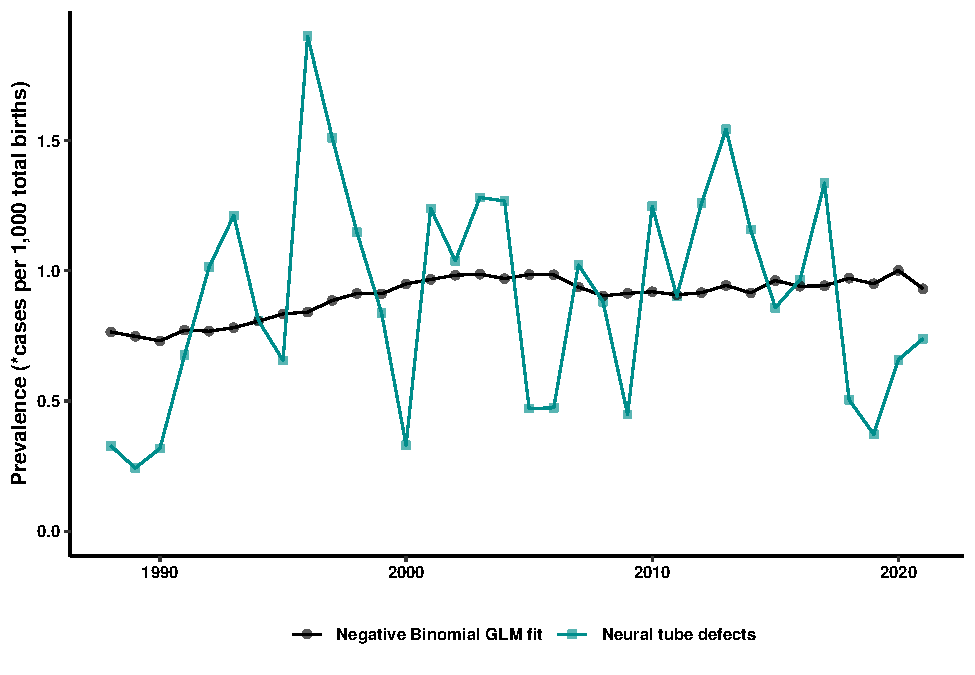
\includegraphics[width=0.65\linewidth,]{02-Trend_files/figure-latex/nt1-1} 

}

\caption{Neural tube defects - Total reported cases.}\label{fig:nt1}
\end{figure}

Based on the statistical analysis, at a \(5\%\) level, it is possible to observe:

\begin{itemize}
\tightlist
\item
  Anencephaly: there is evidence of an increasing trend (\(\hat{\beta_{1}} =\) 0.02, p-value = 0.04).
\end{itemize}

\begin{figure}[h]

{\centering 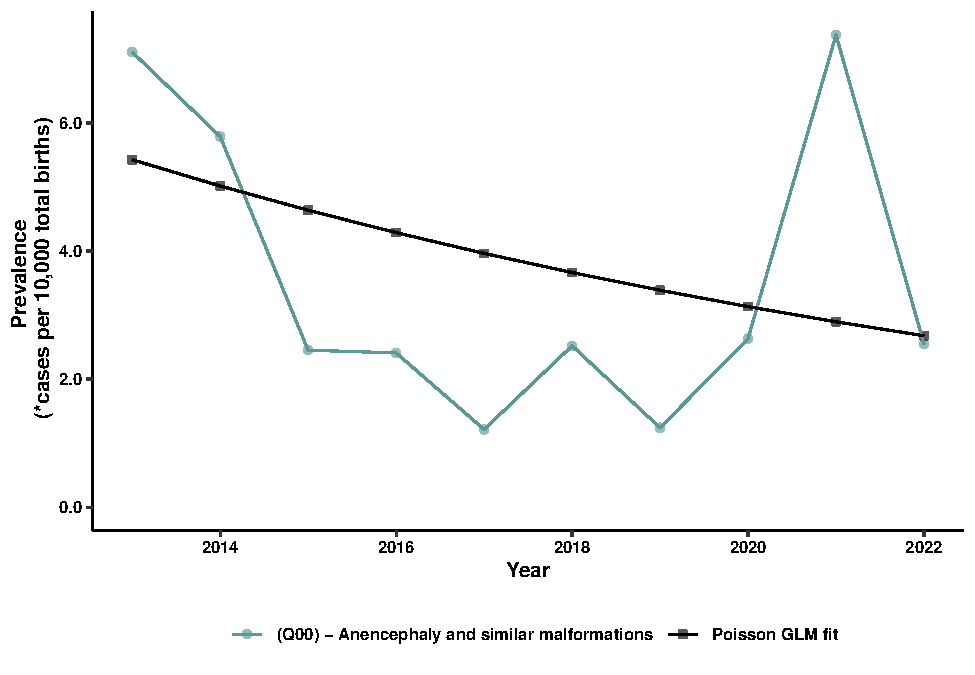
\includegraphics[width=0.65\linewidth,]{02-Trend_files/figure-latex/nt11-1} 

}

\caption{Anencephaly - Total reported cases.}\label{fig:nt11}
\end{figure}

\begin{itemize}
\tightlist
\item
  Encephalocele: there is no significant trend (\(\hat{\beta_{1}} =\) 0.02, p-value = 0.27).
\end{itemize}

\begin{figure}[h]

{\centering 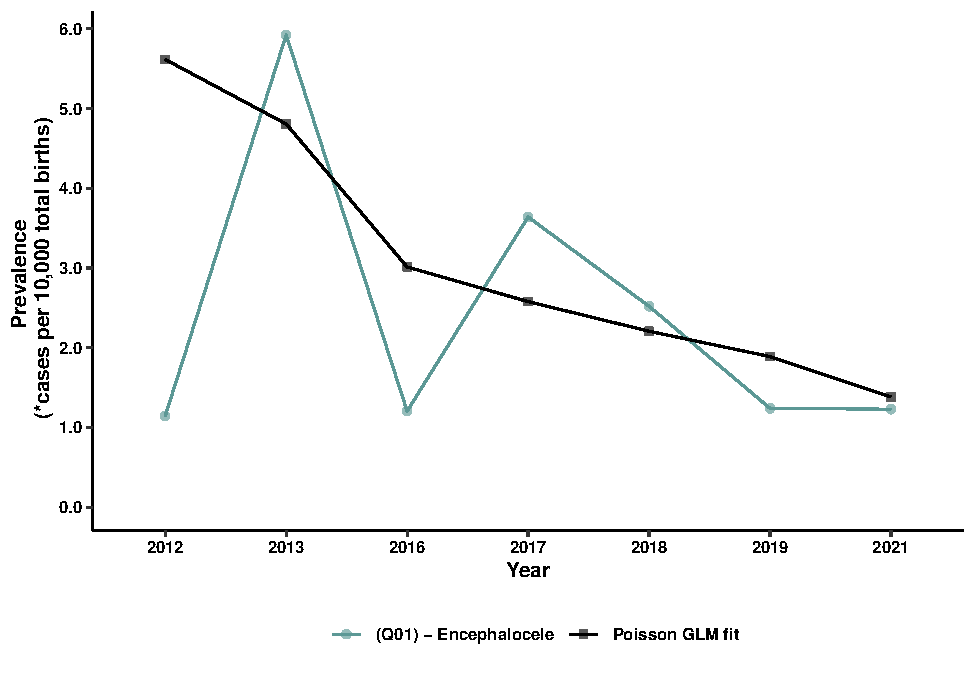
\includegraphics[width=0.65\linewidth,]{02-Trend_files/figure-latex/nt12-1} 

}

\caption{Encephalocele - Total reported cases.}\label{fig:nt12}
\end{figure}

\begin{itemize}
\tightlist
\item
  Spina bifida: there is evidence of a decreasing trend (\(\hat{\beta_{1}} =\) -0.02, p-value = 0.04).
\end{itemize}

\begin{figure}[h]

{\centering 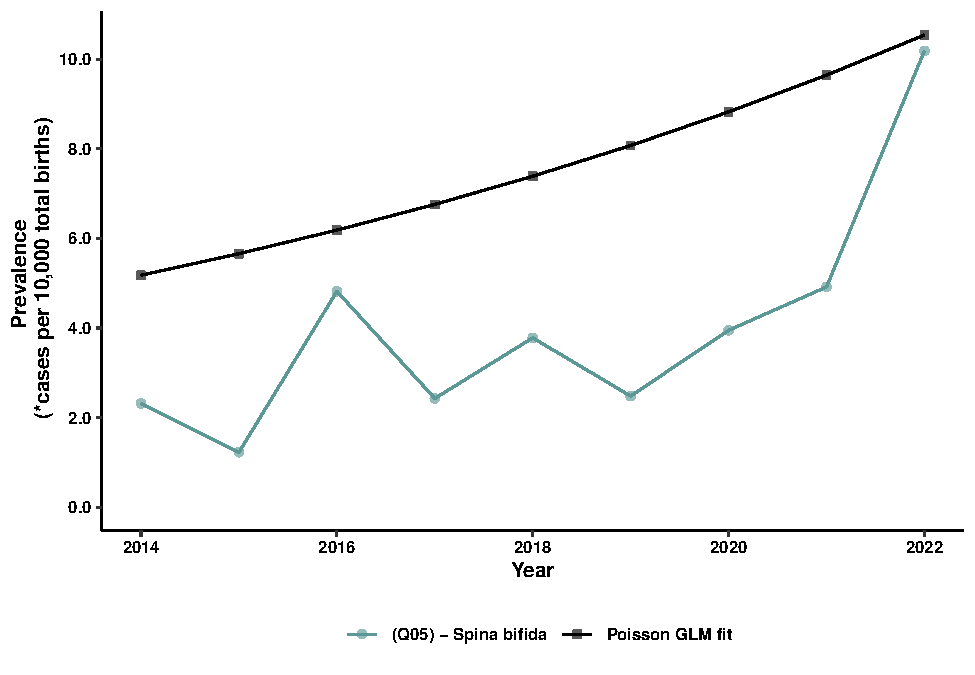
\includegraphics[width=0.65\linewidth,]{02-Trend_files/figure-latex/nt13-1} 

}

\caption{Spina bifida - Total reported cases.}\label{fig:nt13}
\end{figure}

Figure \ref{fig:nt3} shows how the prevalence of neural tube defects is geographically distributed in Nova Scotia by county between 2006 and 2020.

Guysborough is the only county where neural tube defects has never been reported.

In the past, neural tube defects appeared to be more prevalent in northern, western, and eastern counties. Lately, this predominance seems to have concentrated more towards the northern and western counties, with emphasis on Yarmouth, Shelburne, Queens, Hants, and Pictou counties.

\begin{figure}[h]

{\centering 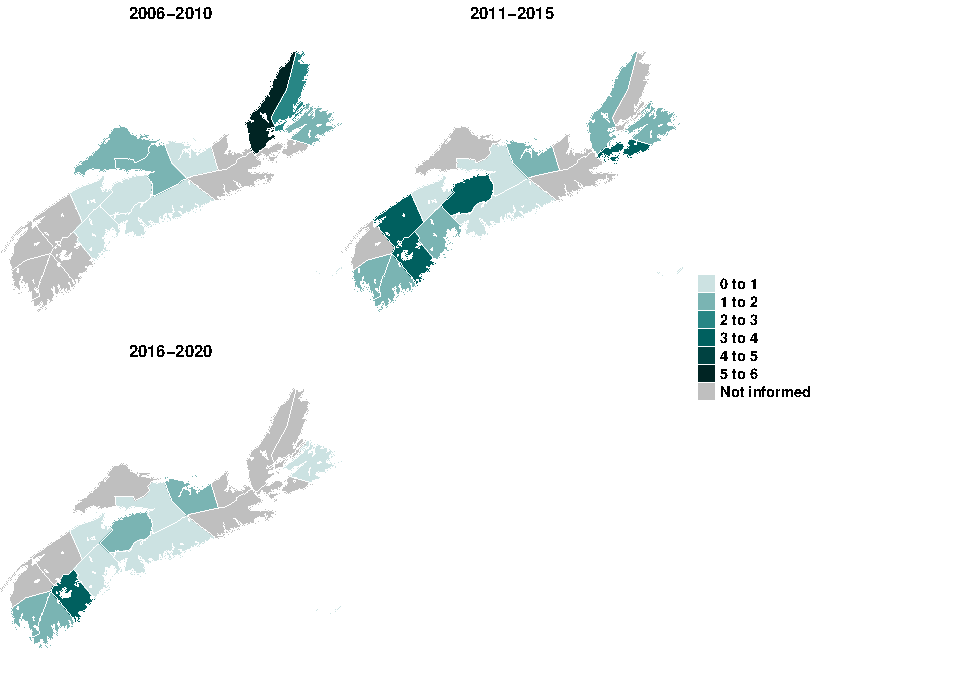
\includegraphics[width=0.65\linewidth,]{02-Trend_files/figure-latex/nt3-1} 

}

\caption{Neural tube defects - Nova Scotia. Shifts in counties between 2006 and 2020.}\label{fig:nt3}
\end{figure}

\clearpage

\hypertarget{section33}{%
\section{Selected central nervous system defects}\label{section33}}

At a \(5\%\) level, there is a decreasing trend for selected central nervous system defects (\(\hat{\beta_{1}} =\) -0.07, p-value = \textless{} 0.0001) for the period 1988 - 2021. From figure \ref{fig:scn1}, the prevalence rate exhibited a sharply upward trend from 1995 to 2000, when it dropped dramatically until 2004. Since then, the rate has gradually fluctuated downwards until reaching the current level.

Over the past 10 years (2012-2021), there is no evidence showing any trend in the prevalence rate of selected central nervous system defects. On average, the prevalence rate for each subsequent year is 0.96 times of the previous year's rate. In other words, the prevalence rate of selected central nervous system defects has been stable by an estimated 4\% over the last decade: (prevalence rate = exp(-0.04) = 0.96 per 1,000 total births; \(\hat{\beta_{1}} =\) -0.04, p-value = 0.13; \(95\%\) CI for \(\hat{\beta_{1}}\) and for the prevalence rate are given by \(CI_{\hat{\beta_{1}}}(95\%)\):{[}-0.09; 0.01{]}, and \(CI_{rate}(95\%)\):{[}0.91; 1.01{]}, respectively).

\begin{figure}[h]

{\centering 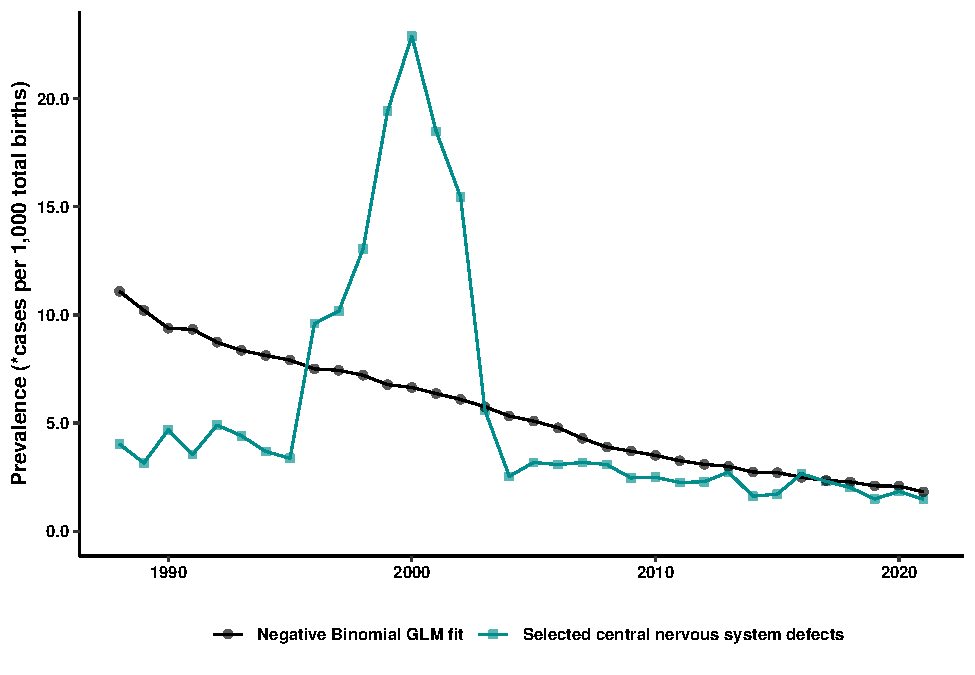
\includegraphics[width=0.65\linewidth,]{02-Trend_files/figure-latex/scn1-1} 

}

\caption{Selected central nervous system defects - Total reported cases.}\label{fig:scn1}
\end{figure}

Based on the statistical analysis, at a \(5\%\) level, it is possible to observe:

\begin{itemize}
\tightlist
\item
  Microcephaly: there is evidence of a decreasing trend (\(\hat{\beta_{1}} =\) -0.08, p-value = \textless{} 0.0001).
\end{itemize}

\begin{figure}[h]

{\centering 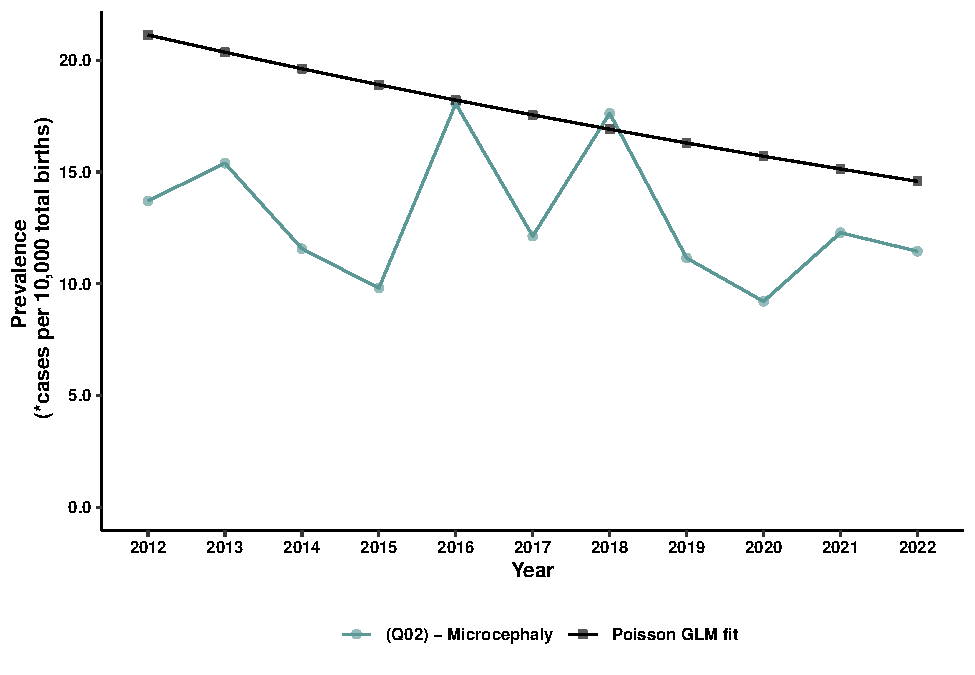
\includegraphics[width=0.65\linewidth,]{02-Trend_files/figure-latex/scn11-1} 

}

\caption{Microcephaly - Total reported cases.}\label{fig:scn11}
\end{figure}

\begin{itemize}
\tightlist
\item
  Congenital hydrocephalus: there is evidence of a decreasing trend (\(\hat{\beta_{1}} =\) -0.03, p-value = \textless{} 0.0001).
\end{itemize}

\begin{figure}[h]

{\centering 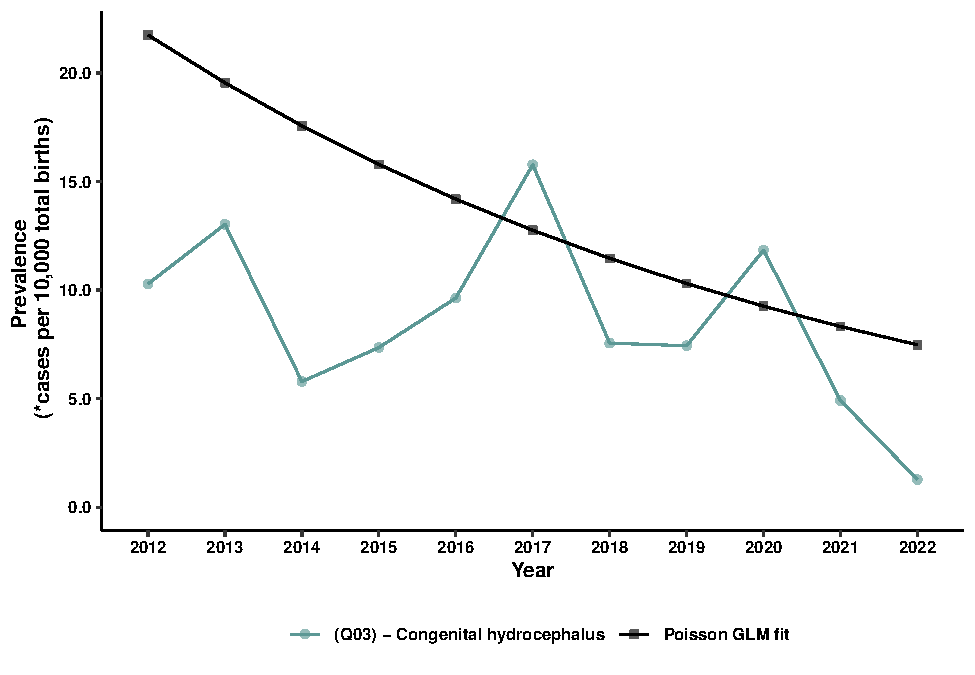
\includegraphics[width=0.65\linewidth,]{02-Trend_files/figure-latex/scn12-1} 

}

\caption{Congenital hydrocephalus - Total reported cases.}\label{fig:scn12}
\end{figure}

\begin{itemize}
\tightlist
\item
  Arhinencephaly/Holoprosencephaly: there is no significant trend (\(\hat{\beta_{1}} =\) 0.01, p-value = 0.67).
\end{itemize}

\begin{figure}[h]

{\centering 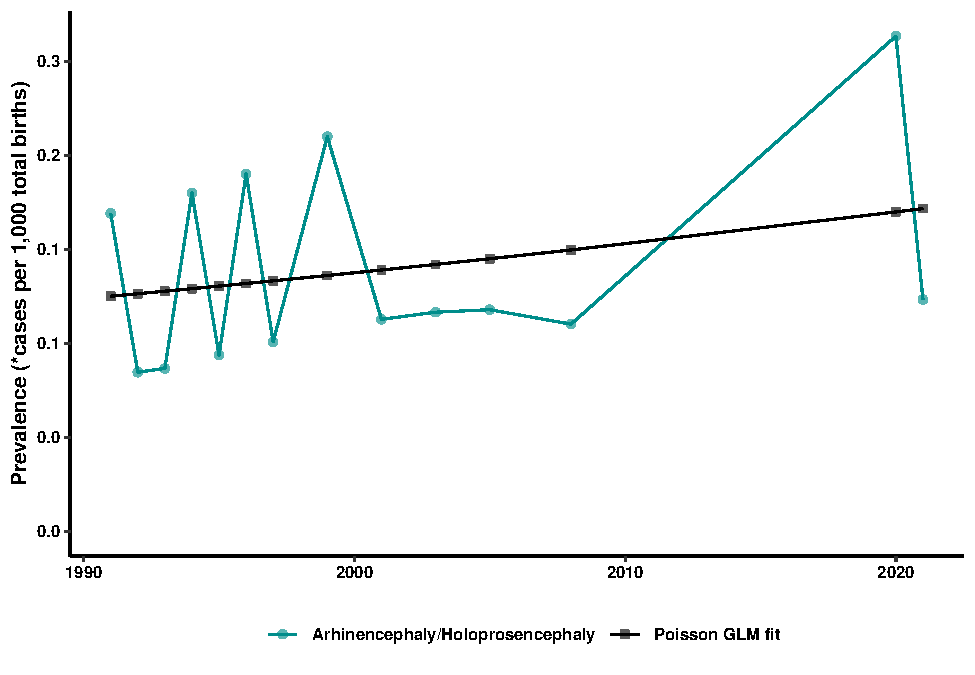
\includegraphics[width=0.65\linewidth,]{02-Trend_files/figure-latex/scn13-1} 

}

\caption{Arhinencephaly/Holoprosencephaly - Total reported cases.}\label{fig:scn13}
\end{figure}

Figure \ref{fig:scn3} shows how the prevalence of selected central nervous system defects is geographically distributed in Nova Scotia by county between 2006 and 2020.

In the past, selected central nervous system defects appeared to be more prevalent in the eastern, and northern counties. Lately, this predominance seems to have concentrated more towards the western counties, with emphasis on Yarmouth, Shelburne, and Queens counties.

\begin{figure}[h]

{\centering 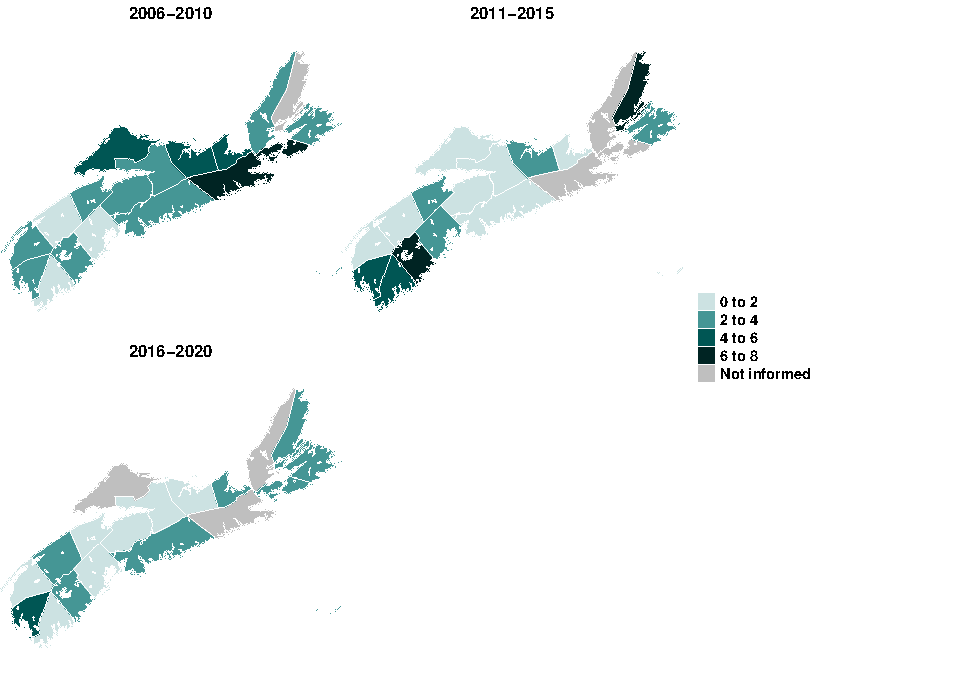
\includegraphics[width=0.65\linewidth,]{02-Trend_files/figure-latex/scn3-1} 

}

\caption{Selected central nervous system defects - Nova Scotia. Shifts in counties between 2006 and 2020.}\label{fig:scn3}
\end{figure}

\clearpage

\hypertarget{section34}{%
\section{Selected sense organ defects}\label{section34}}

At a \(5\%\) level, there is no significant trend for selected sense organ defects (\(\hat{\beta_{1}} =\) -0.003, p-value = 0.72) for the period 1988 - 2021. From figure \ref{fig:ssod1}, the prevalence rate exhibited an upward trend from 1988 to 2003. Since then, the rate has gradually fluctuated downwards until reaching the current level.

Over the past 10 years (2012-2021), there is no evidence showing any trend in the prevalence rate of selected sense organ defects. On average, the prevalence rate for each subsequent year is 0.95 times of the previous year's rate: (prevalence rate = exp(-0.06) = 0.95 per 1,000 total births; \(\hat{\beta_{1}} =\) -0.06, p-value = 0.23; \(95\%\) CI for \(\hat{\beta_{1}}\) and for the prevalence rate are given by \(CI(95\%)_{\hat{\beta_{1}}}\):{[}-0.15; 0.04{]}, and \(CI(95\%)_{rate}\):{[}0.86; 1.04{]}, respectively).

\begin{figure}[h]

{\centering 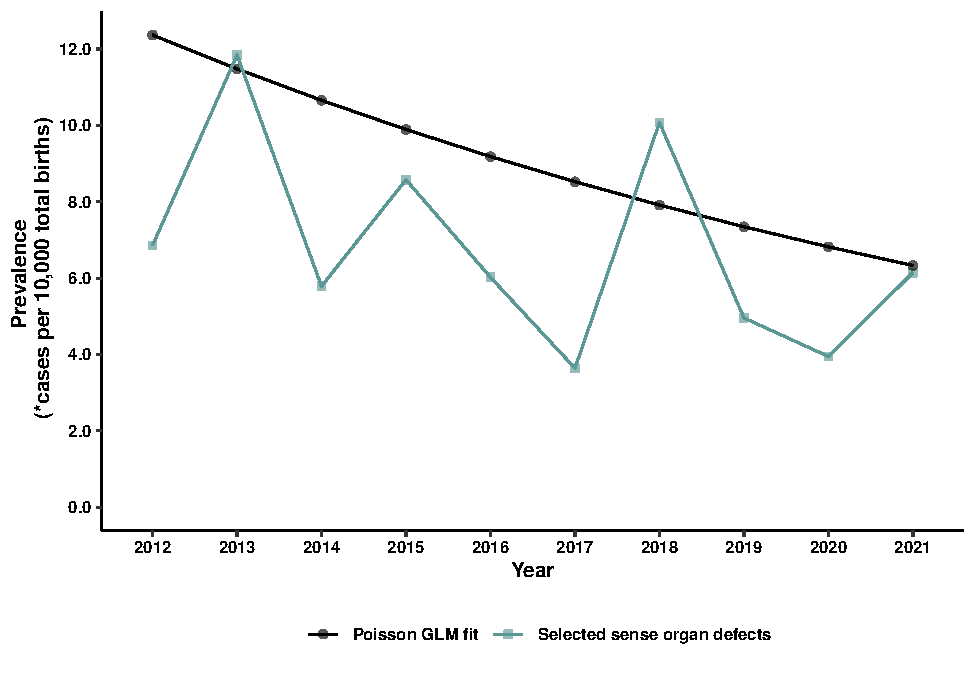
\includegraphics[width=0.9\linewidth,]{02-Trend_files/figure-latex/ssod1-1} 

}

\caption{Selected sense organ defects - Total reported cases.}\label{fig:ssod1}
\end{figure}

Based on the statistical analysis, at a \(5\%\) level, it is possible to observe:

\begin{itemize}
\tightlist
\item
  Anophtalmos/Microphtalmos: there is evidence of a decreasing trend (\(\hat{\beta_{1}} =\) -0.04, p-value = 0.001).
\end{itemize}

\begin{figure}[h]

{\centering 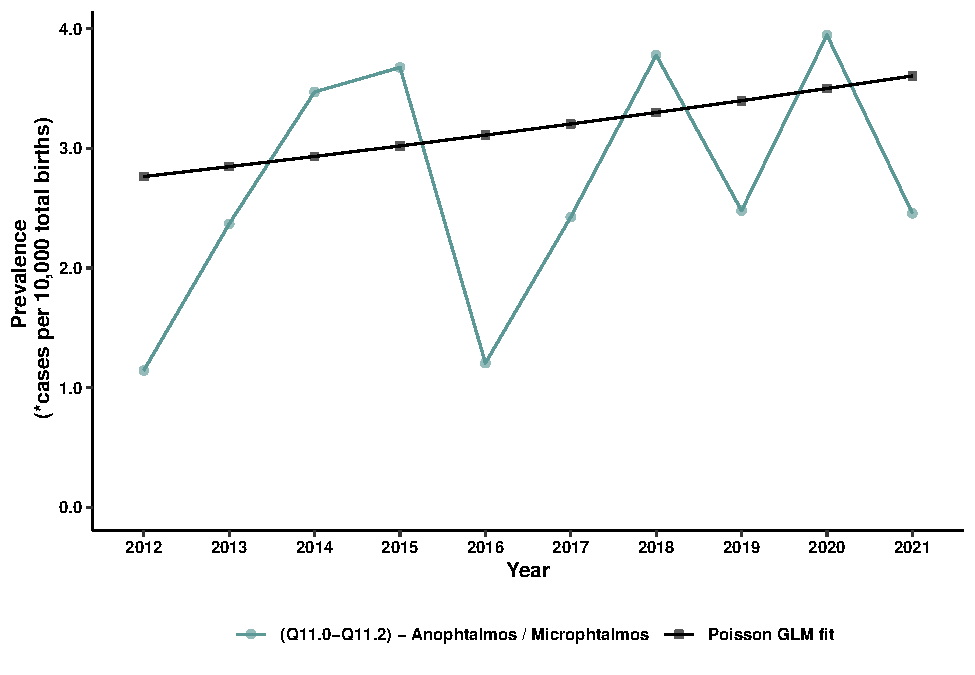
\includegraphics[width=0.65\linewidth,]{02-Trend_files/figure-latex/ssod11-1} 

}

\caption{Anophtalmos/Microphtalmos - Total reported cases.}\label{fig:ssod11}
\end{figure}

\begin{itemize}
\tightlist
\item
  Anotia/Microtia: there is no significant trend (\(\hat{\beta_{1}} =\) 0.02, p-value = 0.32).
\end{itemize}

\begin{figure}[h]

{\centering 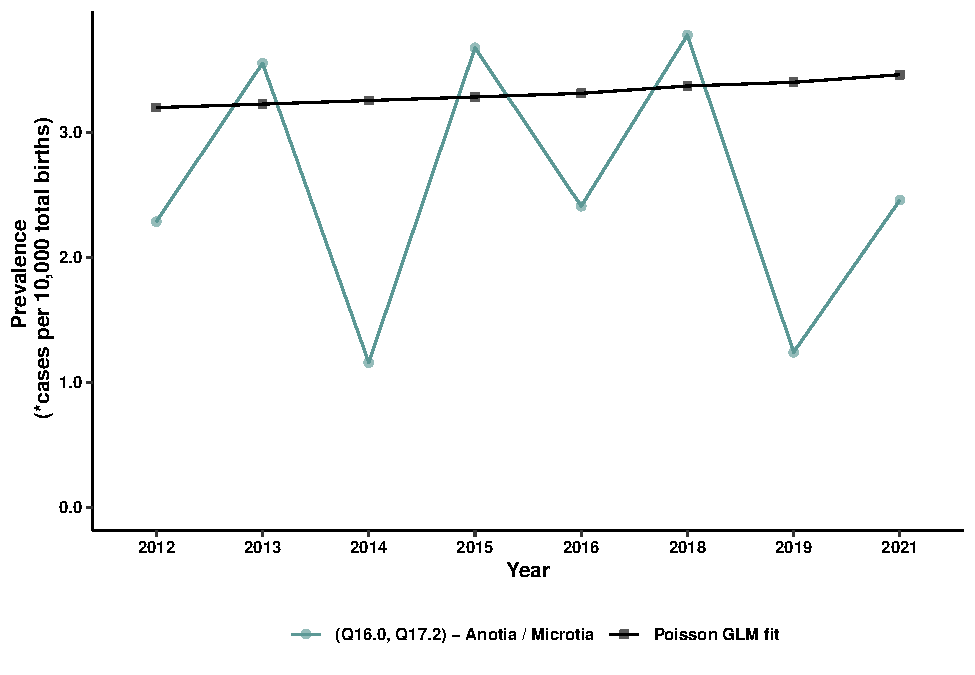
\includegraphics[width=0.65\linewidth,]{02-Trend_files/figure-latex/ssod12-1} 

}

\caption{Anotia/Microtia - Total reported cases.}\label{fig:ssod12}
\end{figure}

\begin{itemize}
\tightlist
\item
  Choanal atresia: there is evidence of a decreasing trend (\(\hat{\beta_{1}} =\) -0.02, p-value = 0.01).
\end{itemize}

\begin{figure}[h]

{\centering 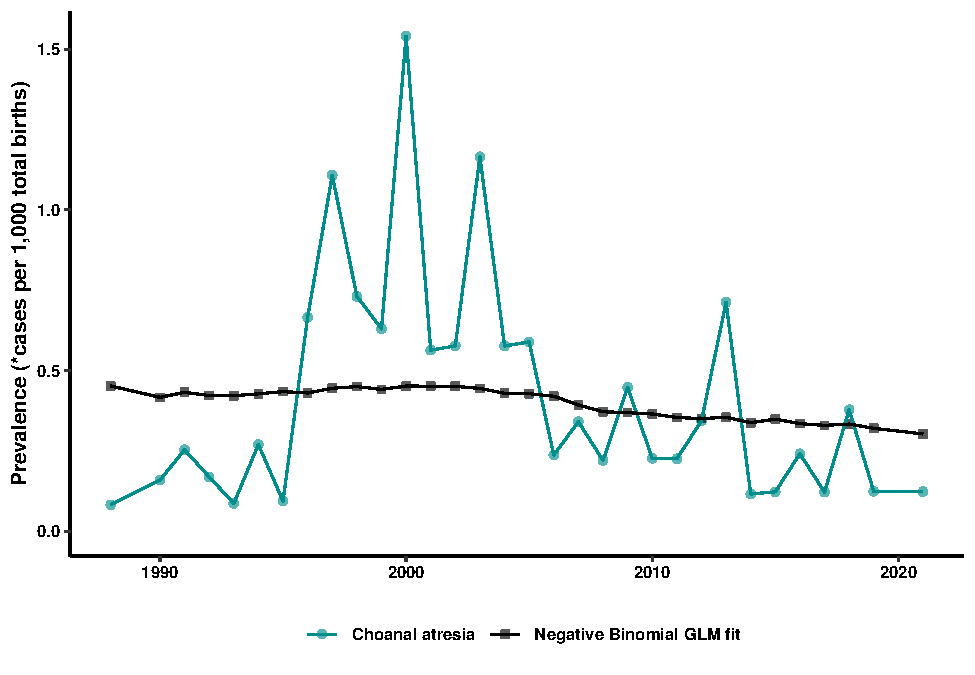
\includegraphics[width=0.65\linewidth,]{02-Trend_files/figure-latex/ssod13-1} 

}

\caption{Choanal atresia - Total reported cases.}\label{fig:ssod13}
\end{figure}

Figure \ref{fig:ssod3} shows how the prevalence of selected sense organ defects is geographically distributed in Nova Scotia by county between 2006 and 2020.

In the past, selected sense organ defects appeared to be more prevalent in northern, western, and central counties. Lately, this predominance seems to have concentrated more towards the northern and western counties, with emphasis on Yarmouth, Shelburne, Kings, and Hants.

\begin{figure}[h]

{\centering 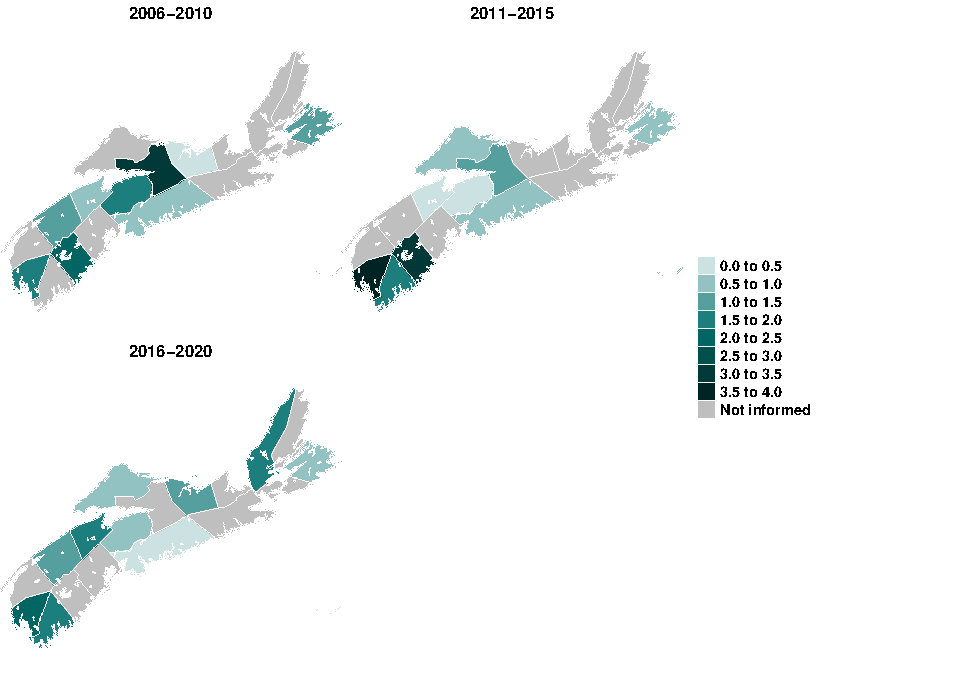
\includegraphics[width=0.65\linewidth,]{02-Trend_files/figure-latex/ssod3-1} 

}

\caption{Selected sense organ defects - Nova Scotia. Shifts in counties between 2006 and 2020.}\label{fig:ssod3}
\end{figure}

\clearpage

\hypertarget{section35}{%
\section{Selected congenital heart defects}\label{section35}}

At a \(5\%\) level, there is no significant trend for selected congenital heart defects (\(\hat{\beta_{1}} =\) -0.004, p-value = 0.22) for the period 1988 - 2021. From figure \ref{fig:schd1}, the prevalence rate exhibited an downward trend from 1988 to 2021 with subsequent peaks being smaller on 1998, 2010, and 2019.

Over the past 10 years (2012-2021), there is no evidence showing any trend in the prevalence rate of selected congenital heart defects. On average, the prevalence rate for each subsequent year is 0.99 times of the previous year's rate: (prevalence rate = exp(-0.01) = 0.99 per 1,000 total births; \(\hat{\beta_{1}} =\) -0.01, p-value = 0.60; \(95\%\) CI for \(\hat{\beta_{1}}\) and for the prevalence rate are given by \(CI(95\%)_{\hat{\beta_{1}}}\):{[}-0.07; 0.04{]}, and \(CI(95\%)_{rate}\):{[}0.94; 1.04{]}, respectively).

\begin{figure}[h]

{\centering 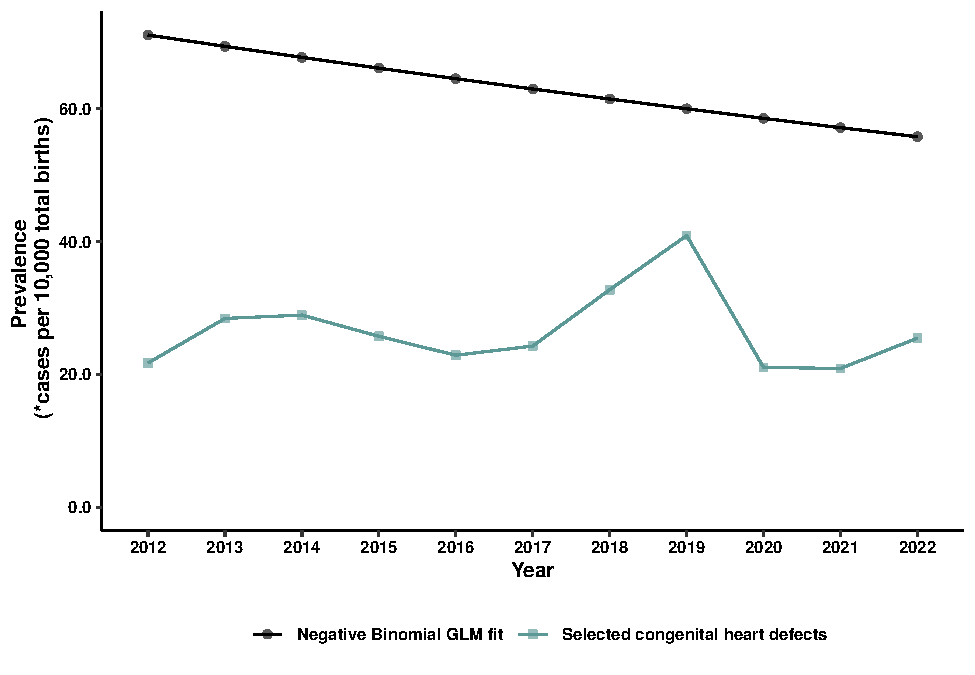
\includegraphics[width=0.9\linewidth,]{02-Trend_files/figure-latex/schd1-1} 

}

\caption{Selected congenital heart defects - Total reported cases.}\label{fig:schd1}
\end{figure}

Based on the statistical analysis, at a \(5\%\) level, it is possible to observe:

\begin{itemize}
\item
  Commom truncus: there is evidence of a decreasing trend (\(\hat{\beta_{1}} =\) -0.04, p-value = 0.02).
\item
  Transposition of great vessels: there is evidence of a decreasing trend (\(\hat{\beta_{1}} =\) -0.01, p-value = 0.01).
\item
  Atrioventricular septal defect: there is no significant trend (\(\hat{\beta_{1}} =\) -0.003, p-value = 0.62).
\item
  Tetralogy of Fallot: there is no significant trend (\(\hat{\beta_{1}} =\) 0.01, p-value = 0.21).
\end{itemize}

\begin{figure}[h]

{\centering 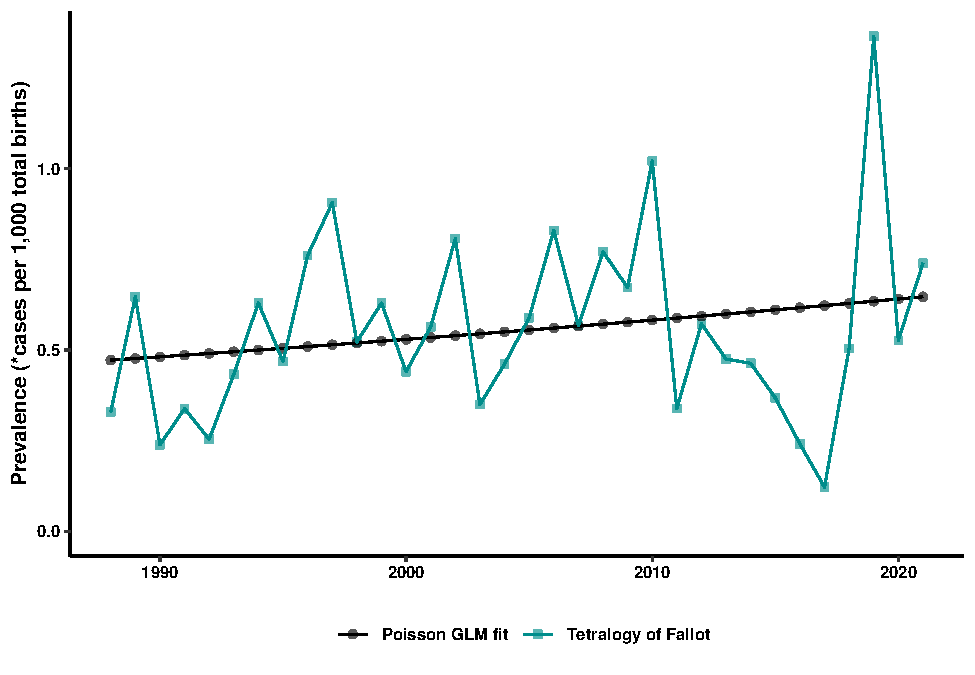
\includegraphics[width=0.65\linewidth,]{02-Trend_files/figure-latex/schd11-1} 

}

\caption{Tetralogy of Fallot - Total reported cases.}\label{fig:schd11}
\end{figure}

\begin{itemize}
\tightlist
\item
  Hypoplastic left heart syndrome: there is no significant trend (\(\hat{\beta_{1}} =\) -0.01, p-value = 0.29).
\end{itemize}

\begin{figure}[h]

{\centering 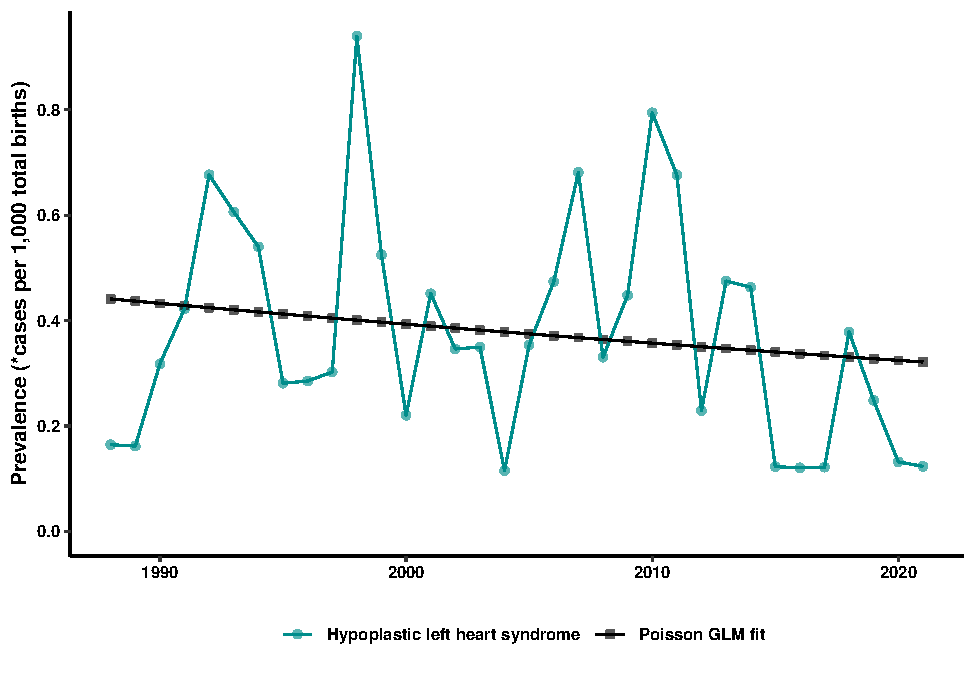
\includegraphics[width=0.65\linewidth,]{02-Trend_files/figure-latex/schd12-1} 

}

\caption{Hypoplastic left heart syndrome - Total reported cases.}\label{fig:schd12}
\end{figure}

\begin{itemize}
\tightlist
\item
  Coarctation of aorta: there is no significant trend (\(\hat{\beta_{1}} =\) 0.003, p-value = 0.62).
\end{itemize}

\begin{figure}[h]

{\centering 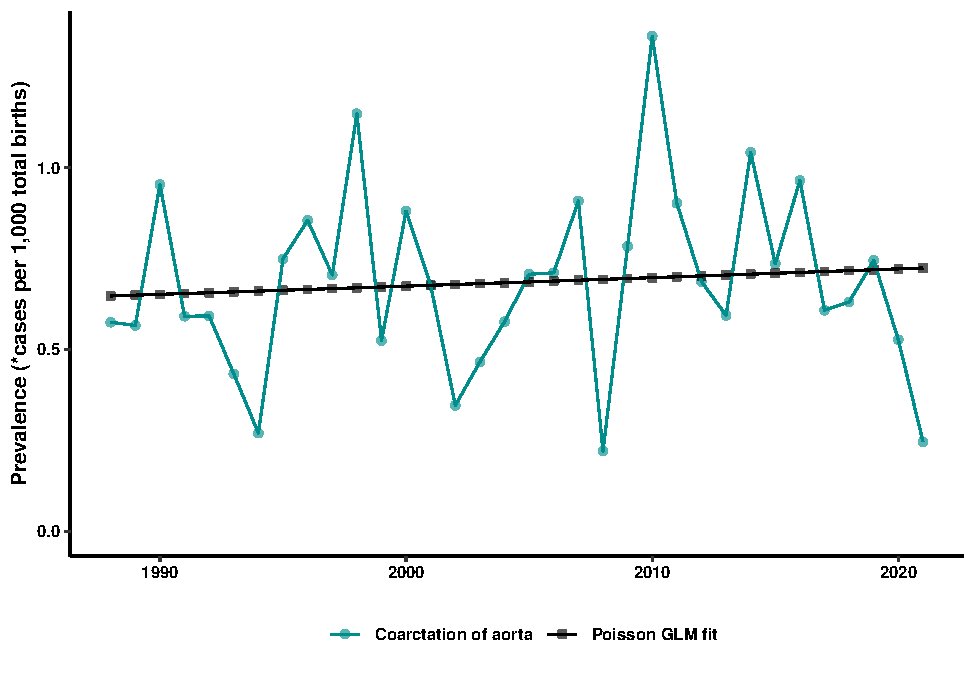
\includegraphics[width=0.65\linewidth,]{02-Trend_files/figure-latex/schd13-1} 

}

\caption{Coarctation of aorta - Total reported cases.}\label{fig:schd13}
\end{figure}

Figure \ref{fig:schd3} shows how the prevalence of selected congenital heart defects is geographically distributed in Nova Scotia by county between 2006 and 2020.

In the past, selected congenital heart defects appeared to be an anomaly that occurred everywhere in the province being more prevalent in the eastern county of Richmond. Lately, this predominance seems to have consolidated and other eastern counties like Inverness and Victoria are also showing a high prevalence rate for selected congenital heart defects.

\begin{figure}[h]

{\centering 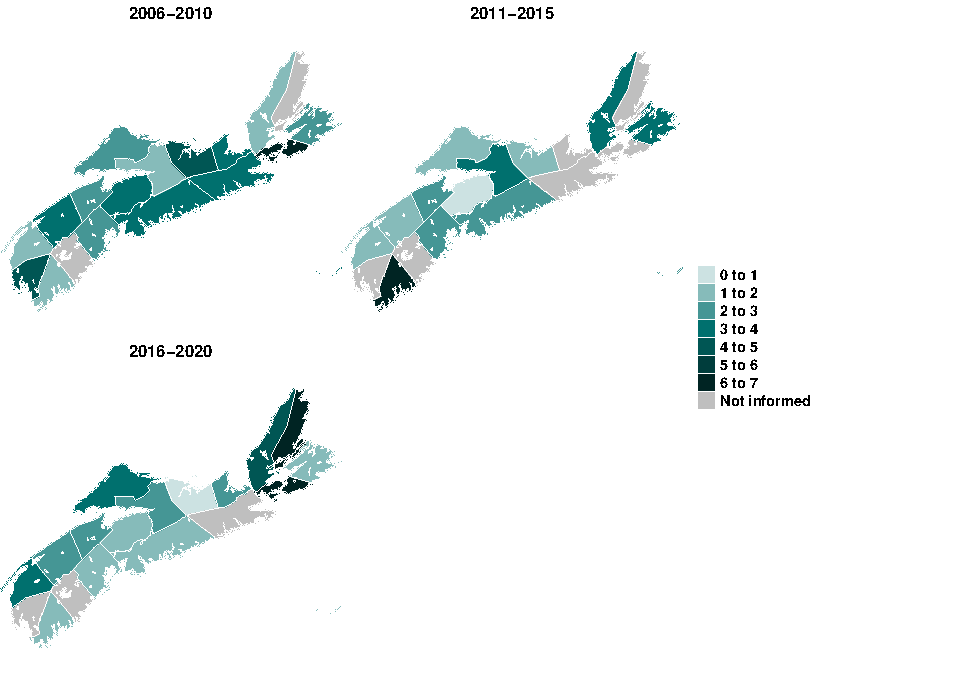
\includegraphics[width=0.65\linewidth,]{02-Trend_files/figure-latex/schd3-1} 

}

\caption{Selected congenital heart defects - Nova Scotia. Shifts in counties between 2006 and 2020.}\label{fig:schd3}
\end{figure}

\clearpage

\hypertarget{section36}{%
\section{Oro-facial clefts}\label{section36}}

At a \(5\%\) level, there is no significant trend for oro-facial clefts (\(\hat{\beta_{1}} =\) -0.002, p-value = 0.65) for the period 1988 - 2021. From figure \ref{fig:ofc1}, the prevalence rate exhibited an upward trend from 1988 to 2011 with drastic lower rates between 2012 and 2021.

Over the past 10 years (2012-2021), there is no evidence showing any trend in the prevalence rate of oro-facial clefts. On average, the prevalence rate for each subsequent year is 1.03 times of the previous year's rate: (prevalence rate = exp(0.03) = 1.03 per 1,000 total births; \(\hat{\beta_{1}} =\) 0.03, p-value = 0.31; \(95\%\) CI for \(\hat{\beta_{1}}\) and for the prevalence rate are given by \(CI(95\%)_{\hat{\beta_{1}}}\):{[}-0.03; 0.10{]}, and \(CI(95\%)_{rate}\):{[}0.97; 1.10{]}, respectively).

\begin{figure}[h]

{\centering 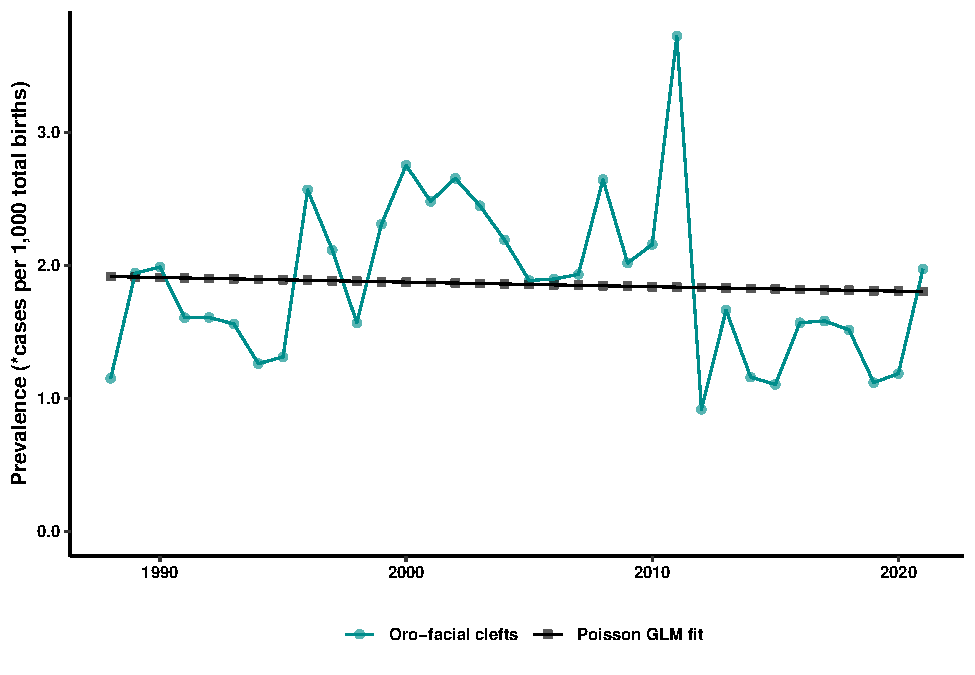
\includegraphics[width=0.9\linewidth,]{02-Trend_files/figure-latex/ofc1-1} 

}

\caption{Oro-facial clefts - Total reported cases.}\label{fig:ofc1}
\end{figure}

Based on the statistical analysis, at a \(5\%\) level, it is possible to observe:

\begin{itemize}
\tightlist
\item
  Cleft palate only: there is no significant trend (\(\hat{\beta_{1}} =\) 0.003, p-value = 0.66).
\end{itemize}

\begin{figure}[h]

{\centering 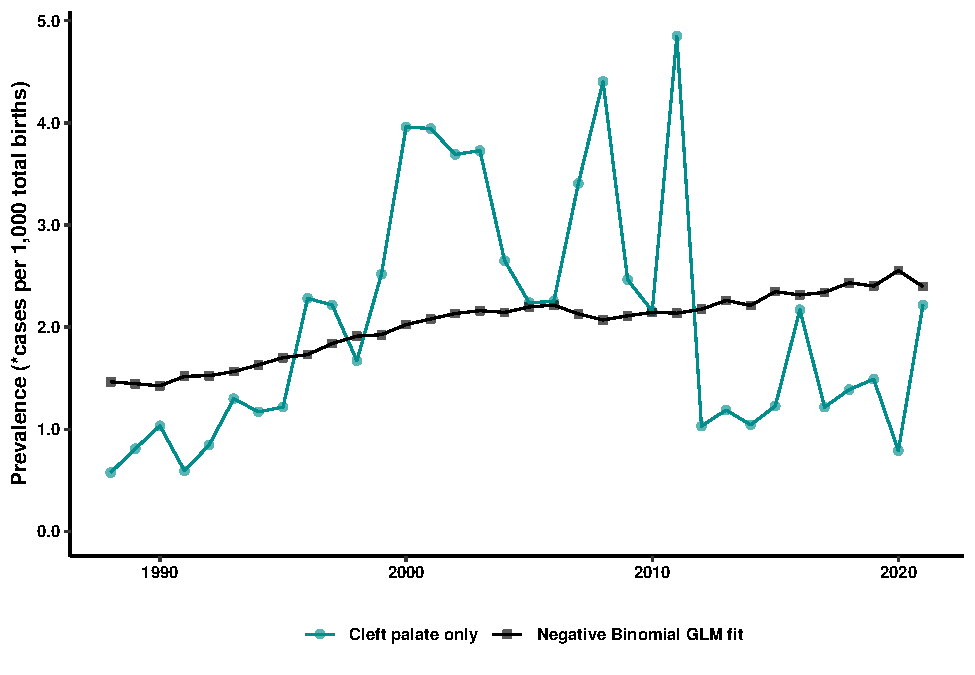
\includegraphics[width=0.65\linewidth,]{02-Trend_files/figure-latex/ofc11-1} 

}

\caption{Cleft palate only - Total reported cases.}\label{fig:ofc11}
\end{figure}

\begin{itemize}
\tightlist
\item
  Cleft lip only: there is no significant trend (\(\hat{\beta_{1}} =\) -0.02, p-value = 0.07).
\end{itemize}

\begin{figure}[h]

{\centering 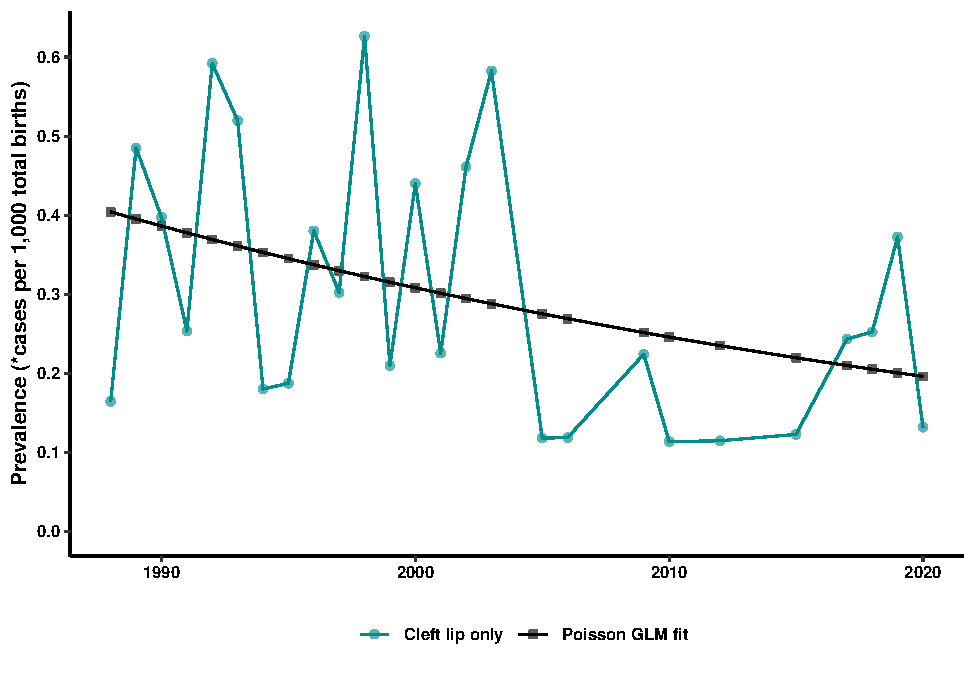
\includegraphics[width=0.65\linewidth,]{02-Trend_files/figure-latex/ofc12-1} 

}

\caption{Cleft lip only - Total reported cases.}\label{fig:ofc12}
\end{figure}

\begin{itemize}
\tightlist
\item
  Cleft palate with cleft lip: there is no significant trend (\(\hat{\beta_{1}} =\) 0.002, p-value = 0.74).
\end{itemize}

\begin{figure}[h]

{\centering 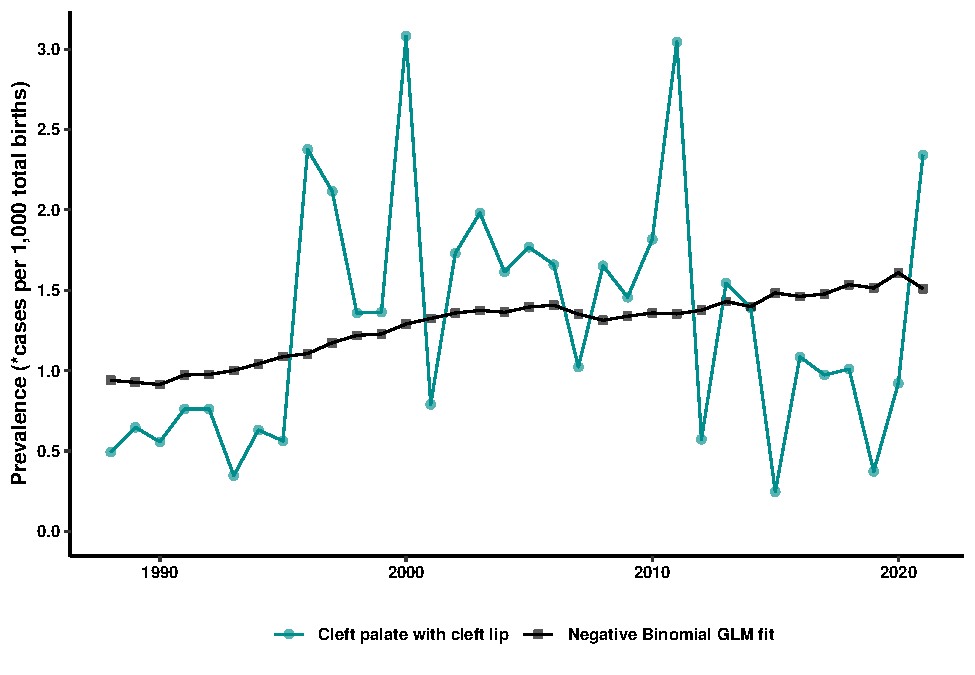
\includegraphics[width=0.65\linewidth,]{02-Trend_files/figure-latex/ofc13-1} 

}

\caption{Cleft palate with cleft lip - Total reported cases.}\label{fig:ofc13}
\end{figure}

Figure \ref{fig:ofc3} shows how the prevalence of oro-facial clefts is geographically distributed in Nova Scotia by county between 2006 and 2020.

In the past, oro-facial clefts appeared to be more prevalent in northern, central, and eastern counties. Lately, this predominance seems to have concentrated more towards the northern and western counties, with emphasis on Yarmouth, Hants, and Colchester counties. In the eastern side of the province, Victoria county has the highest levels.

\begin{figure}[h]

{\centering 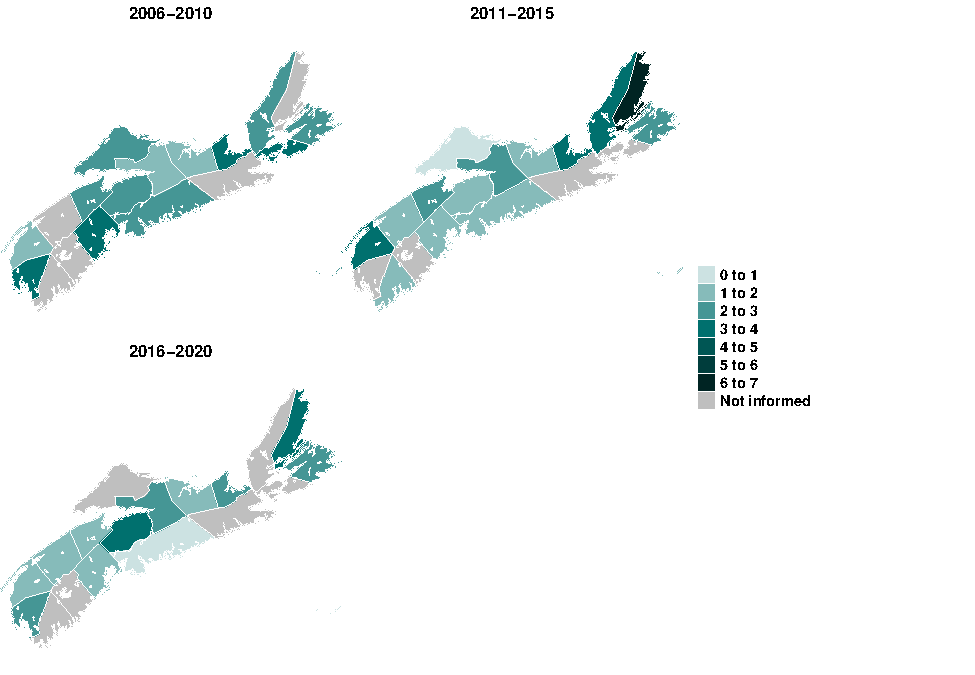
\includegraphics[width=0.65\linewidth,]{02-Trend_files/figure-latex/ofc3-1} 

}

\caption{Oro-facial clefts - Nova Scotia. Shifts in counties between 2006 and 2020.}\label{fig:ofc3}
\end{figure}

\clearpage

\hypertarget{section37}{%
\section{Selected gastrointestinal defects}\label{section37}}

At a \(5\%\) level, there is an increasing trend for selected gastrointestinal defects (\(\hat{\beta_{1}} =\) 0.01, p-value = 0.001) for the period 1988 - 2021. From figure \ref{fig:sgd1}, the prevalence rate exhibited an upward trend from 1988 to 2005, while it has oscillated between highs and lows since then.

Over the past 10 years (2012-2021), there is no evidence showing any trend in the prevalence rate of selected gastrointestinal defects. On average, the prevalence rate for each subsequent year is 1.00 times of the previous year's rate: (prevalence rate = exp(0.005) = 1.005 per 1,000 total births; \(\hat{\beta_{1}} =\) 0.00, p-value = 0.88; \(95\%\) CI for \(\hat{\beta_{1}}\) and for the prevalence rate are given by \(CI(95\%)_{\hat{\beta_{1}}}\):{[}-0.06; 0.07{]}, and \(CI(95\%)_{rate}\):{[}0.95; 1.07{]}, respectively).

\begin{figure}[h]

{\centering 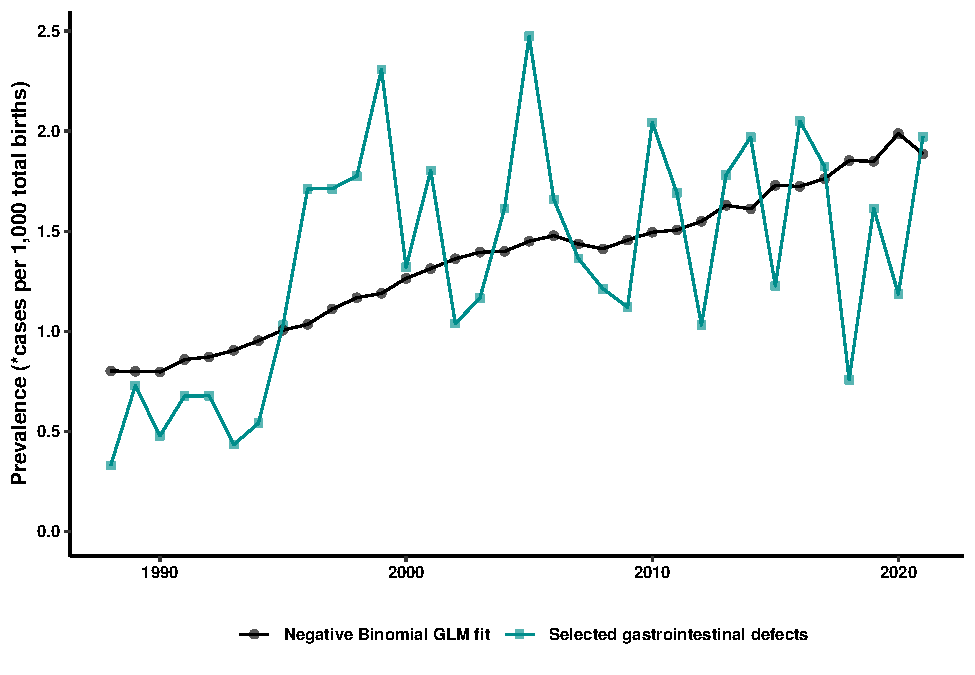
\includegraphics[width=0.9\linewidth,]{02-Trend_files/figure-latex/sgd1-1} 

}

\caption{Selected gastrointestinal defects - Total reported cases.}\label{fig:sgd1}
\end{figure}

Based on the statistical analysis, at a \(5\%\) level, it is possible to observe:

\begin{itemize}
\tightlist
\item
  Oesophageal atresia/stenosis, tracheoesophageal fistula: there is no significant trend (\(\hat{\beta_{1}} =\) 0.01, p-value = 0.11).
\end{itemize}

\begin{figure}[h]

{\centering 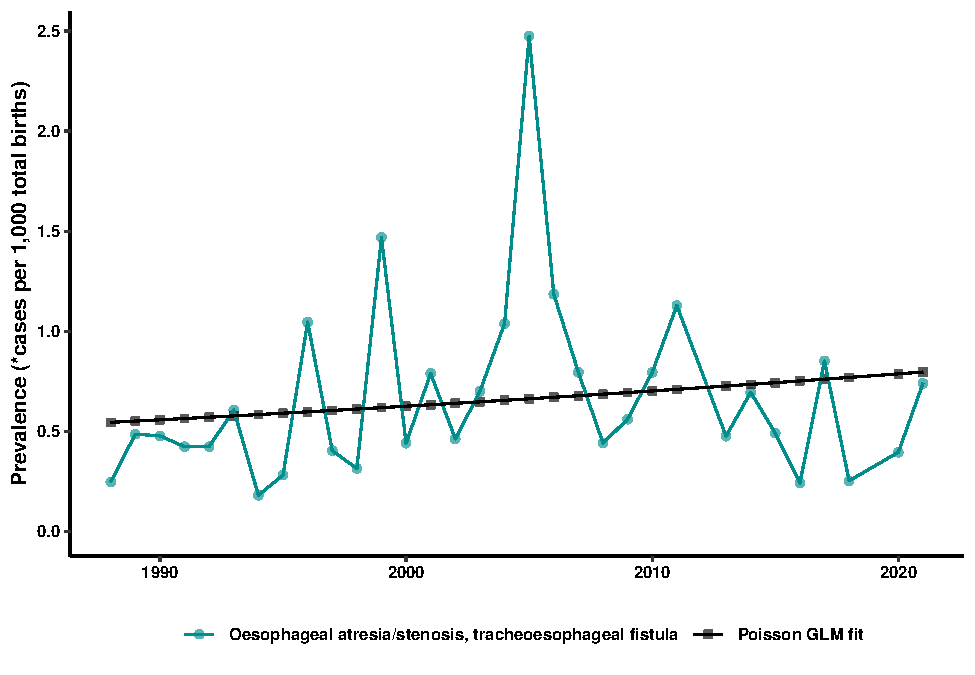
\includegraphics[width=0.65\linewidth,]{02-Trend_files/figure-latex/sgd11-1} 

}

\caption{Oesophageal atresia/stenosis, tracheoesophageal fistula - Total reported cases.}\label{fig:sgd11}
\end{figure}

\begin{itemize}
\tightlist
\item
  Small intestine absence/atresia/stenosis: there is no significant trend (\(\hat{\beta_{1}} =\) 0.01, p-value = 0.53).
\end{itemize}

\begin{figure}[h]

{\centering 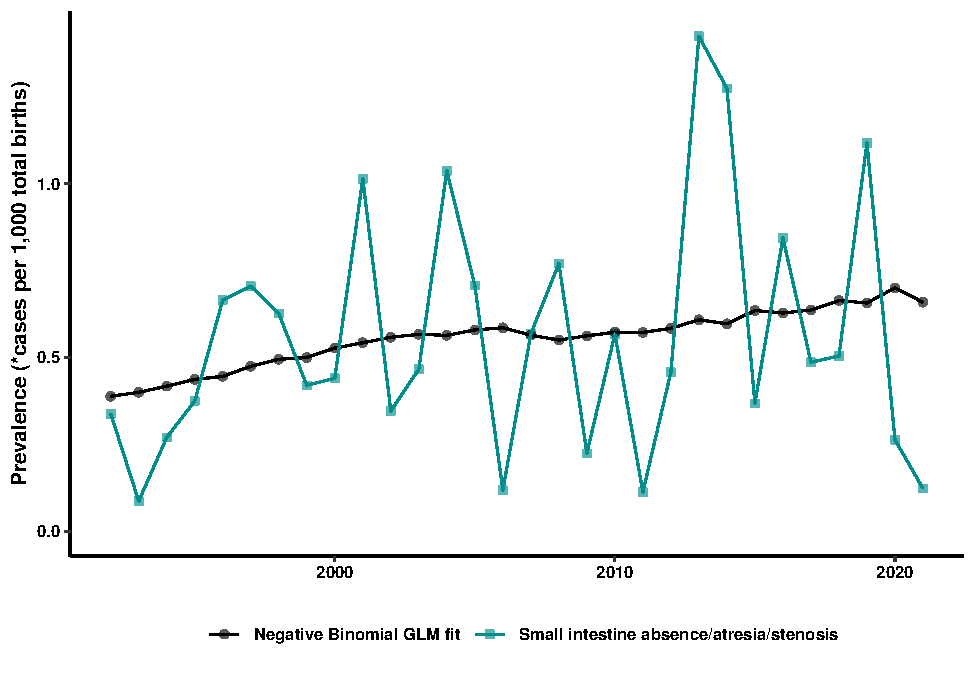
\includegraphics[width=0.65\linewidth,]{02-Trend_files/figure-latex/sgd12-1} 

}

\caption{Small intestine absence/atresia/stenosis - Total reported cases.}\label{fig:sgd12}
\end{figure}

\begin{itemize}
\tightlist
\item
  Ano-rectal absence/atresia/stenosis: there is evidence of an increasing trend (\(\hat{\beta_{1}} =\) 0.04, p-value = 0.005).
\end{itemize}

\begin{figure}[h]

{\centering 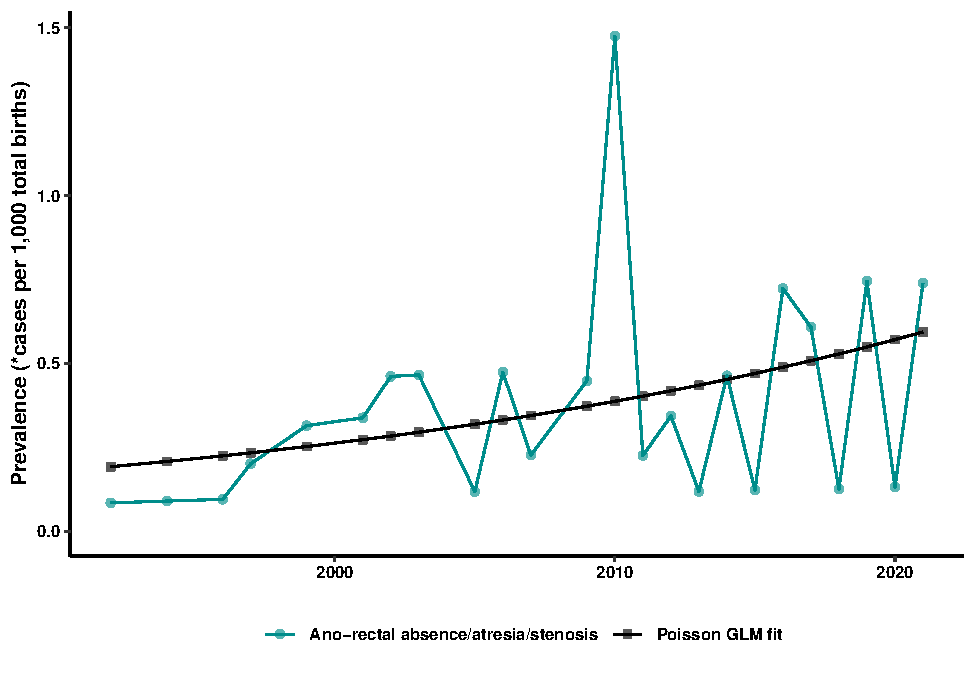
\includegraphics[width=0.65\linewidth,]{02-Trend_files/figure-latex/sgd13-1} 

}

\caption{Ano-rectal absence/atresia/stenosis - Total reported cases.}\label{fig:sgd13}
\end{figure}

\begin{itemize}
\tightlist
\item
  Hirschsprung disease: there is no significant trend (\(\hat{\beta_{1}} =\) 0.01, p-value = 0.29).
\end{itemize}

\begin{figure}[h]

{\centering 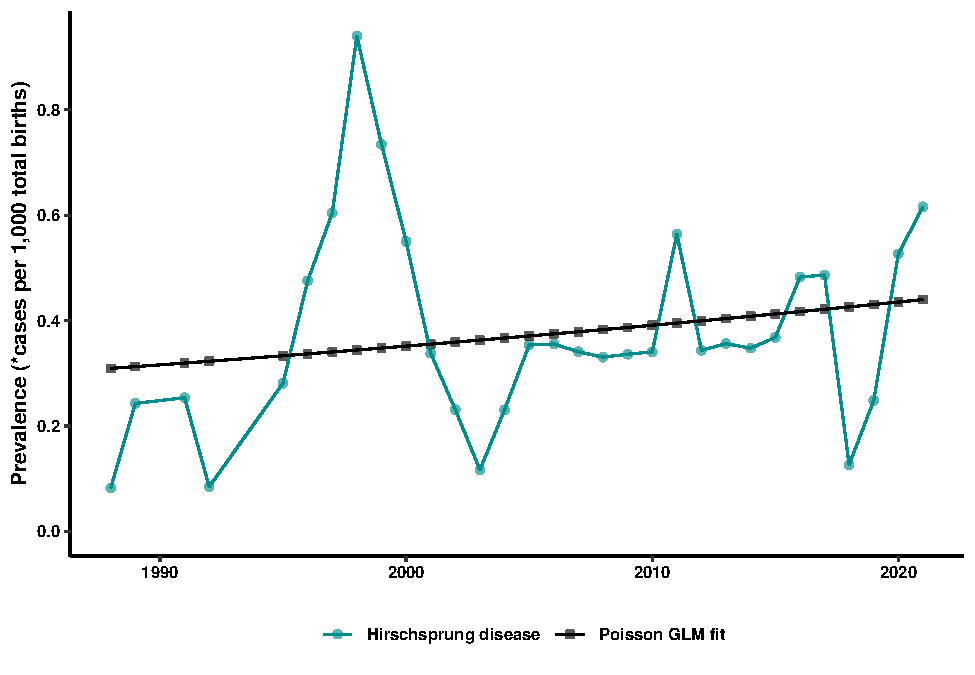
\includegraphics[width=0.65\linewidth,]{02-Trend_files/figure-latex/sgd14-1} 

}

\caption{Hirschsprung disease - Total reported cases.}\label{fig:sgd14}
\end{figure}

\begin{itemize}
\tightlist
\item
  Atresia of bile ducts: there is no significant trend (\(\hat{\beta_{1}} =\) 0.01, p-value = 0.43).
\end{itemize}

\begin{figure}[h]

{\centering 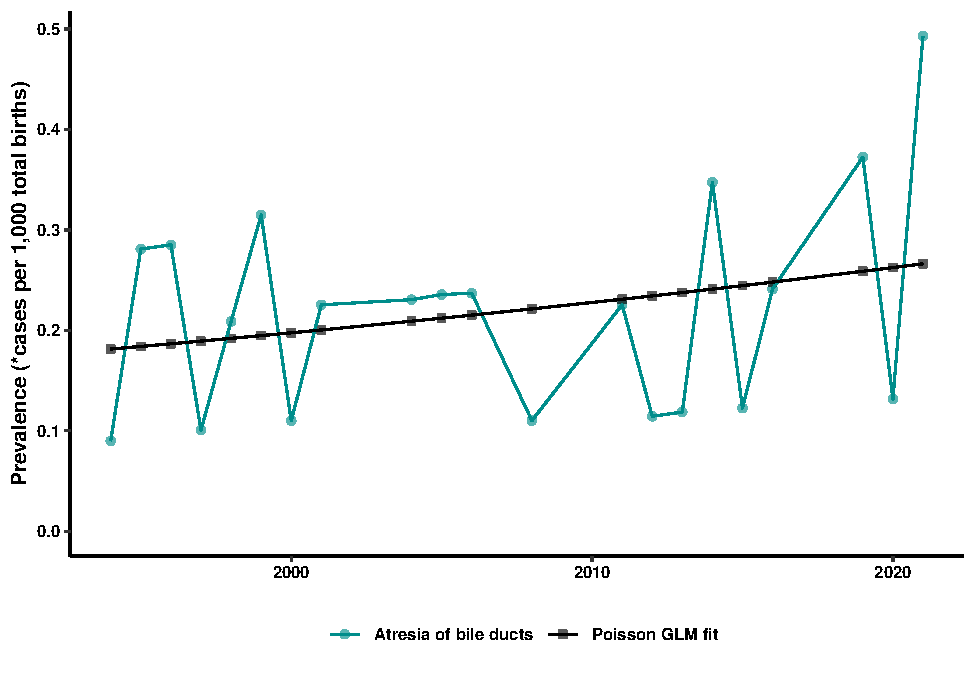
\includegraphics[width=0.65\linewidth,]{02-Trend_files/figure-latex/sgd15-1} 

}

\caption{Atresia of bile ducts - Total reported cases.}\label{fig:sgd15}
\end{figure}

Figure \ref{fig:sgd3} shows how the prevalence of selected gastrointestinal defects is geographically distributed in Nova Scotia by county between 2006 and 2020.

In the past, selected gastrointestinal defects was found to be more prevalent in northern, western, and eastern counties. Presently, the prevalence distribution remains similar, with an emphasis on the counties of Yarmouth, Digby, Inverness and Richmond.

\begin{figure}[h]

{\centering 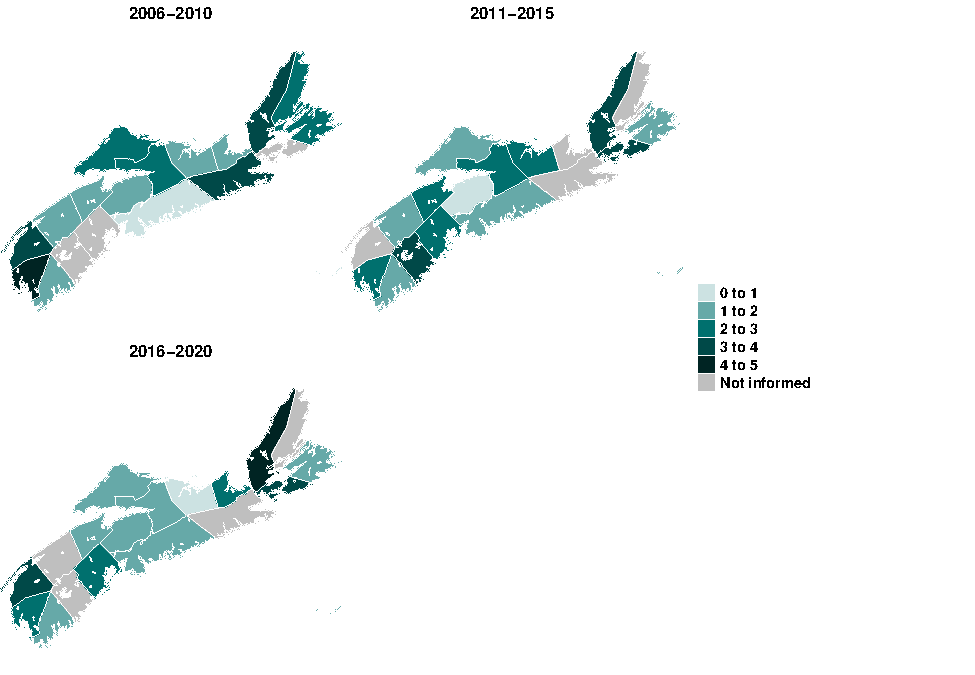
\includegraphics[width=0.65\linewidth,]{02-Trend_files/figure-latex/sgd3-1} 

}

\caption{Selected gastrointestinal defects - Nova Scotia. Shifts in counties between 2006 and 2020.}\label{fig:sgd3}
\end{figure}

\clearpage

\hypertarget{section38}{%
\section{Selected genital anomalies}\label{section38}}

At a \(5\%\) level, there is an increasing trend for selected genital anomalies (\(\hat{\beta_{1}} =\) 0.01, p-value = 0.03) for the period 1988 - 2021. From figure \ref{fig:sga1}, the prevalence rate has been exhibiting an upward trend with the peaks getting higher over the years.

Over the past 10 years (2012-2021), there is no evidence showing any trend in the prevalence rate of selected genital anomalies. On average, the prevalence rate for each subsequent year is 1.02 times of the previous year's rate: (prevalence rate = exp(0.02) = 1.02 per 1,000 total births; \(\hat{\beta_{1}} =\) 0.02, p-value = 0.19; \(95\%\) CI for \(\hat{\beta_{1}}\) and for the prevalence rate are given by \(CI(95\%)_{\hat{\beta_{1}}}\):{[}-0.01; 0.05{]}, and \(CI(95\%)_{rate}\):{[}0.99; 1.05{]}, respectively).

\begin{figure}[h]

{\centering 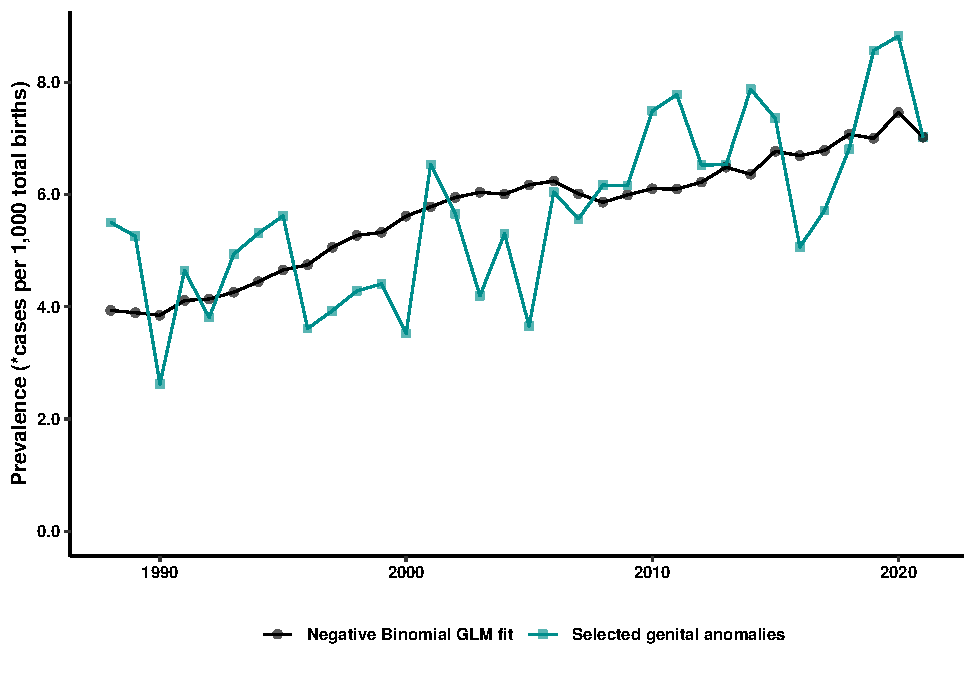
\includegraphics[width=0.9\linewidth,]{02-Trend_files/figure-latex/sga1-1} 

}

\caption{Selected genital anomalies - Total reported cases.}\label{fig:sga1}
\end{figure}

Based on the statistical analysis, at a \(5\%\) level, it is possible to observe:

\begin{itemize}
\tightlist
\item
  Cryptorchidism/undescended testicles: there is evidence of a decreasing trend (\(\hat{\beta_{1}} =\) -0.02, p-value = \textless{} 0.0001).
\end{itemize}

\begin{figure}[h]

{\centering 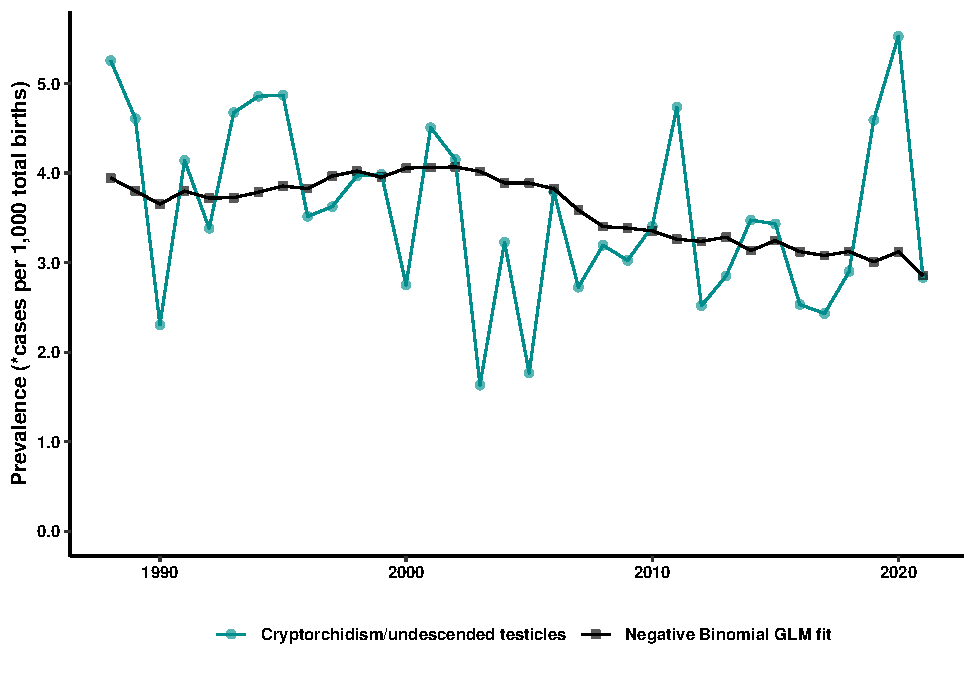
\includegraphics[width=0.65\linewidth,]{02-Trend_files/figure-latex/sga11-1} 

}

\caption{Cryptorchidism/undescended testicles - Total reported cases.}\label{fig:sga11}
\end{figure}

\begin{itemize}
\tightlist
\item
  Hypospadias: there is evidence of an increasing trend (\(\hat{\beta_{1}} =\) 0.10, p-value = \textless{} 0.0001).
\end{itemize}

\begin{figure}[h]

{\centering 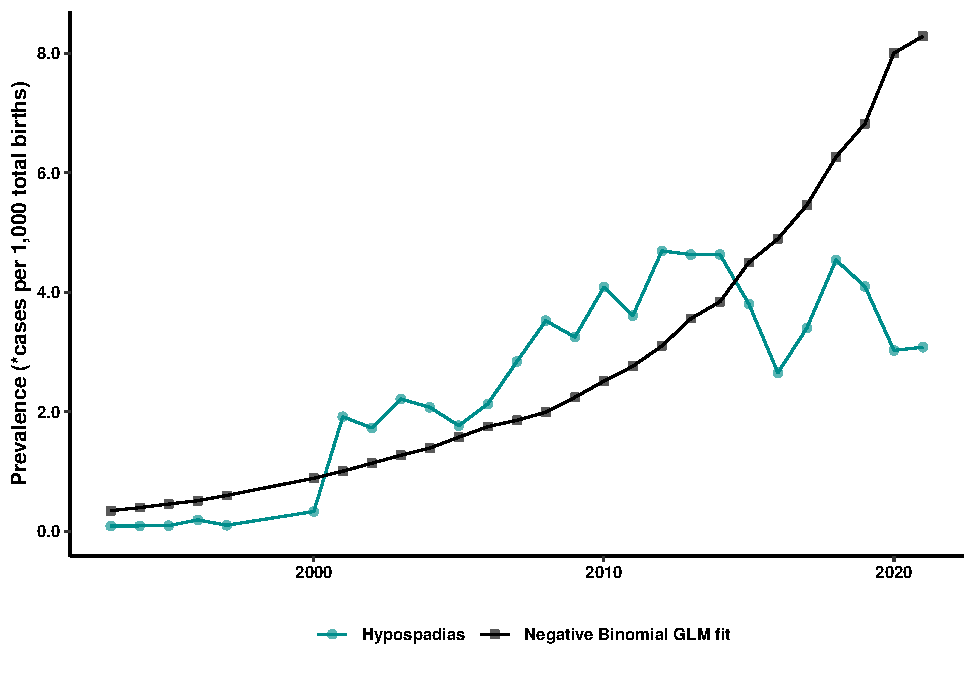
\includegraphics[width=0.65\linewidth,]{02-Trend_files/figure-latex/sga12-1} 

}

\caption{Hypospadias - Total reported cases.}\label{fig:sga12}
\end{figure}

\begin{itemize}
\tightlist
\item
  Indeterminate sex: there is no significant trend (\(\hat{\beta_{1}} =\) -0.01, p-value = 0.53).
\end{itemize}

\begin{figure}[h]

{\centering 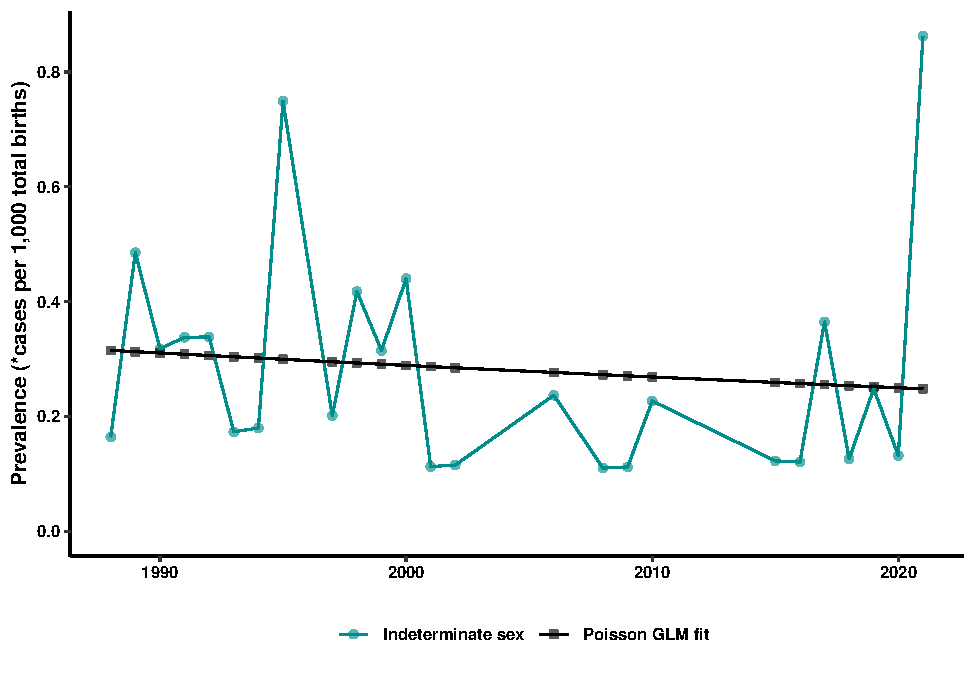
\includegraphics[width=0.65\linewidth,]{02-Trend_files/figure-latex/sga13-1} 

}

\caption{Indeterminate sex - Total reported cases.}\label{fig:sga13}
\end{figure}

\begin{itemize}
\tightlist
\item
  Epispadias: there is no significant trend (\(\hat{\beta_{1}} =\) 0.01, p-value = 0.62).
\end{itemize}

\begin{figure}[h]

{\centering 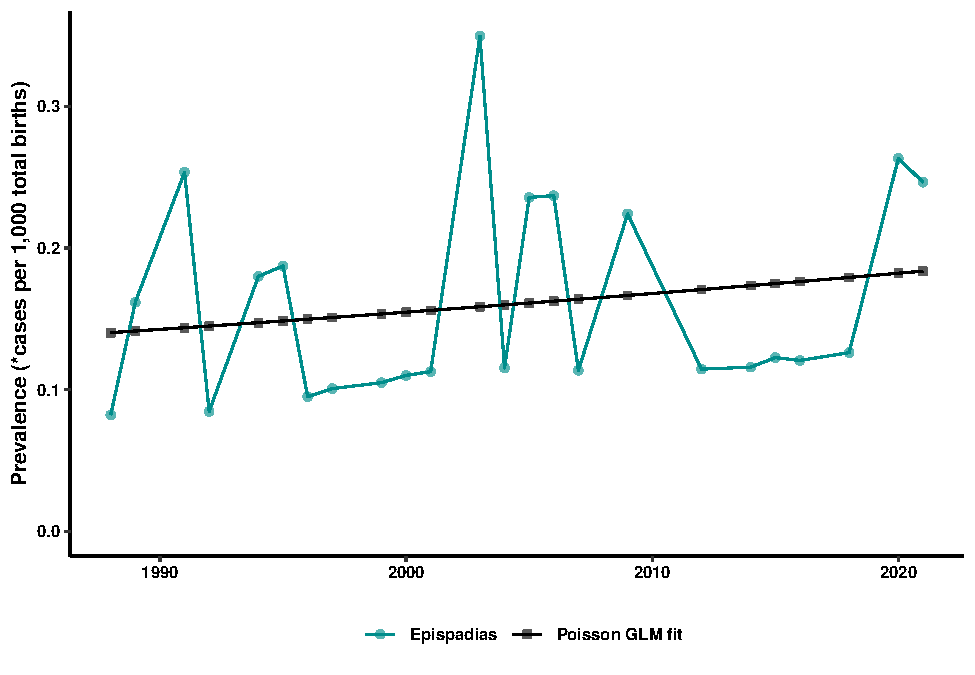
\includegraphics[width=0.65\linewidth,]{02-Trend_files/figure-latex/sga14-1} 

}

\caption{Epispadias - Total reported cases.}\label{fig:sga14}
\end{figure}

Figure \ref{fig:sga3} shows how the prevalence of selected genital anomalies is geographically distributed in Nova Scotia by county between 2006 and 2020.

In the past, selected genital anomalies appeared to be more prevalent in western, and eastern counties. Lately, this predominance seems to have spread to the entire province with emphasis on Yarmouth, Digby, Queens, Pictou and Guysborough counties.

\begin{figure}[h]

{\centering 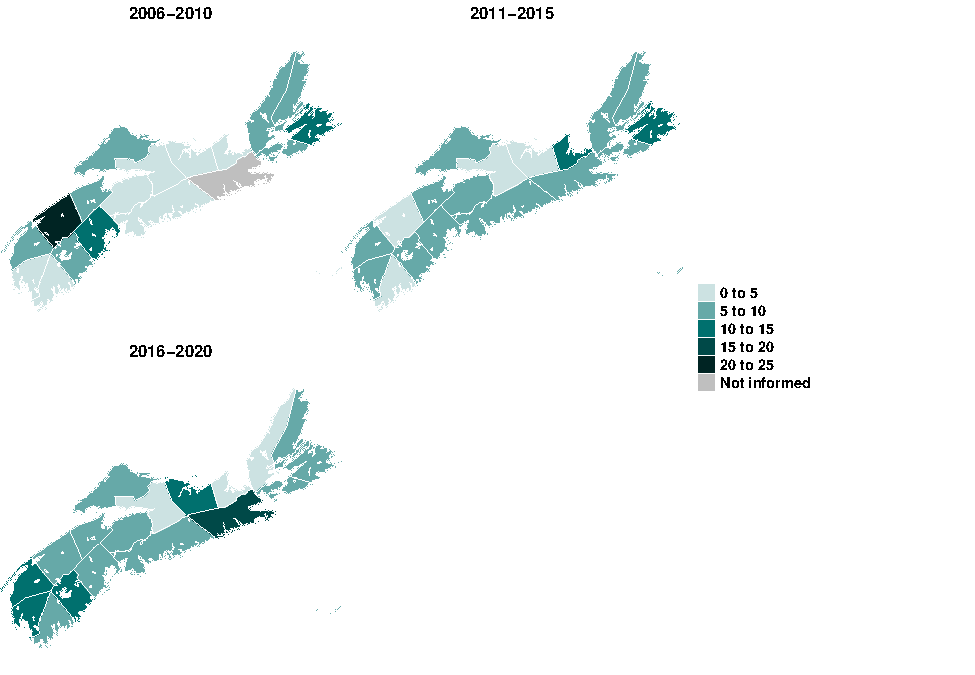
\includegraphics[width=0.65\linewidth,]{02-Trend_files/figure-latex/sga3-1} 

}

\caption{Selected genital anomalies - Nova Scotia. Shifts in counties between 2006 and 2020.}\label{fig:sga3}
\end{figure}

\clearpage

\hypertarget{section39}{%
\section{Selected urinary tract defects}\label{section39}}

At a \(5\%\) level, there is an increasing trend for selected urinary tract defects (\(\hat{\beta_{1}} =\) 0.02, p-value = \textless{} 0.0001) for the period 1988 - 2021. From figure \ref{fig:sutd1}, the prevalence rate exhibited an upward trend from 1988 to 2000. Since then, it has oscillated with highs and lows with no clear direction.

Over the past 10 years (2012-2021), there is no evidence showing any trend in the prevalence rate of selected urinary tract defects. On average, the prevalence rate for each subsequent year is 1.02 times of the previous year's rate: (prevalence rate = exp(0.02) = 1.02 per 1,000 total births; \(\hat{\beta_{1}} =\) 0.02, p-value = 0.58; \(95\%\) CI for \(\hat{\beta_{1}}\) and for the prevalence rate are given by \(CI(95\%)_{\hat{\beta_{1}}}\):{[}-0.04; 0.07{]}, and \(CI(95\%)_{rate}\):{[}0.96; 1.07{]}, respectively).

\begin{figure}[h]

{\centering 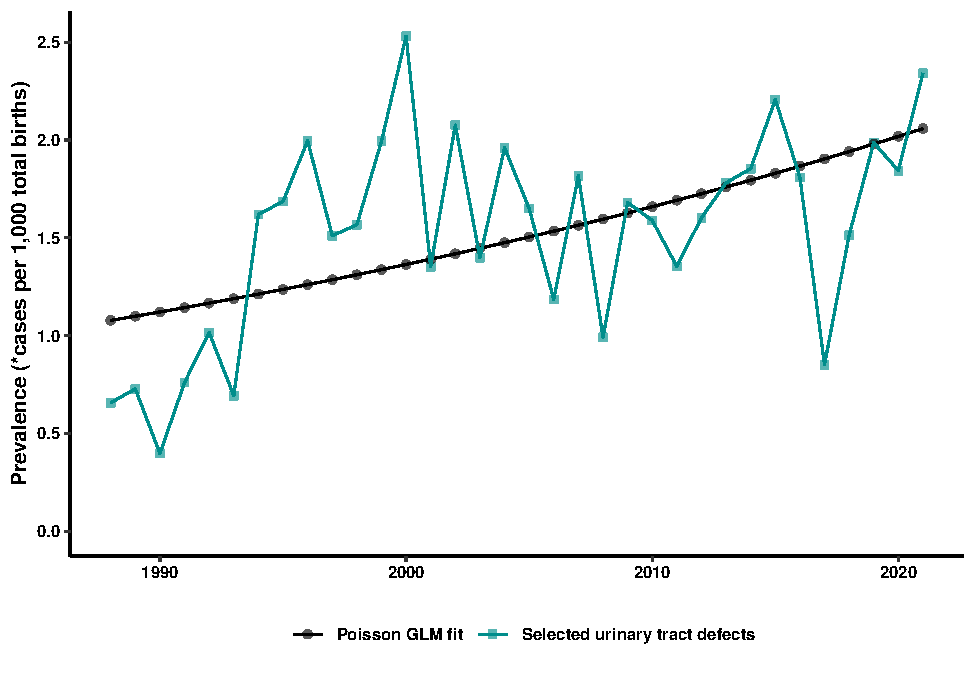
\includegraphics[width=0.9\linewidth,]{02-Trend_files/figure-latex/sutd1-1} 

}

\caption{Selected urinary tract defects - Total reported cases.}\label{fig:sutd1}
\end{figure}

Based on the statistical analysis, at a \(5\%\) level, it is possible to observe:

\begin{itemize}
\tightlist
\item
  Renal agenesis: there is evidence of an increasing trend (\(\hat{\beta_{1}} =\) 0.02, p-value = 0.03).
\end{itemize}

\begin{figure}[h]

{\centering 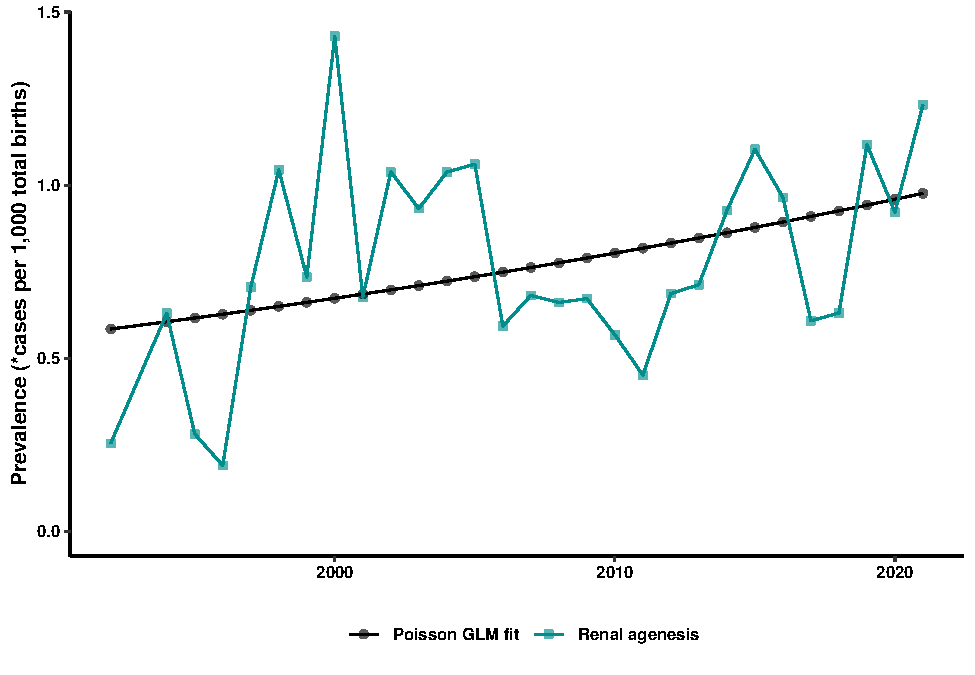
\includegraphics[width=0.65\linewidth,]{02-Trend_files/figure-latex/sutd11-1} 

}

\caption{Renal agenesis - Total reported cases.}\label{fig:sutd11}
\end{figure}

\begin{itemize}
\tightlist
\item
  Cystic kidney: there is no significant trend (\(\hat{\beta_{1}} =\) 0.01, p-value = 0.29).
\end{itemize}

\begin{figure}[h]

{\centering 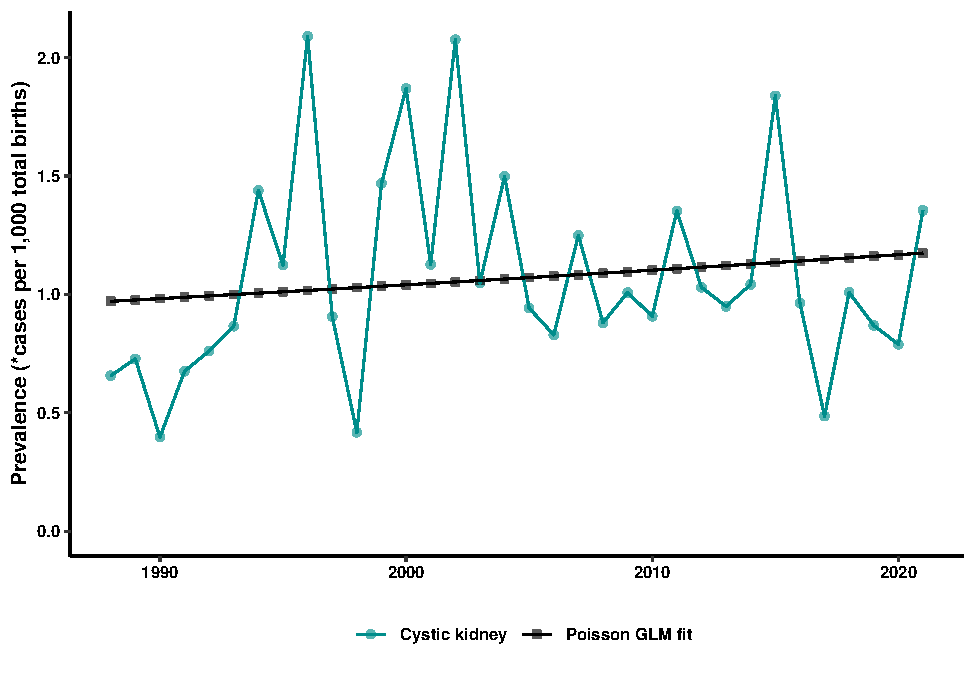
\includegraphics[width=0.65\linewidth,]{02-Trend_files/figure-latex/sutd12-1} 

}

\caption{Cystic kidney - Total reported cases.}\label{fig:sutd12}
\end{figure}

\begin{itemize}
\tightlist
\item
  Bladder and cloacal exstrophy: there is no significant trend (\(\hat{\beta_{1}} =\) 0.01, p-value = 0.53).
\end{itemize}

\begin{figure}[h]

{\centering 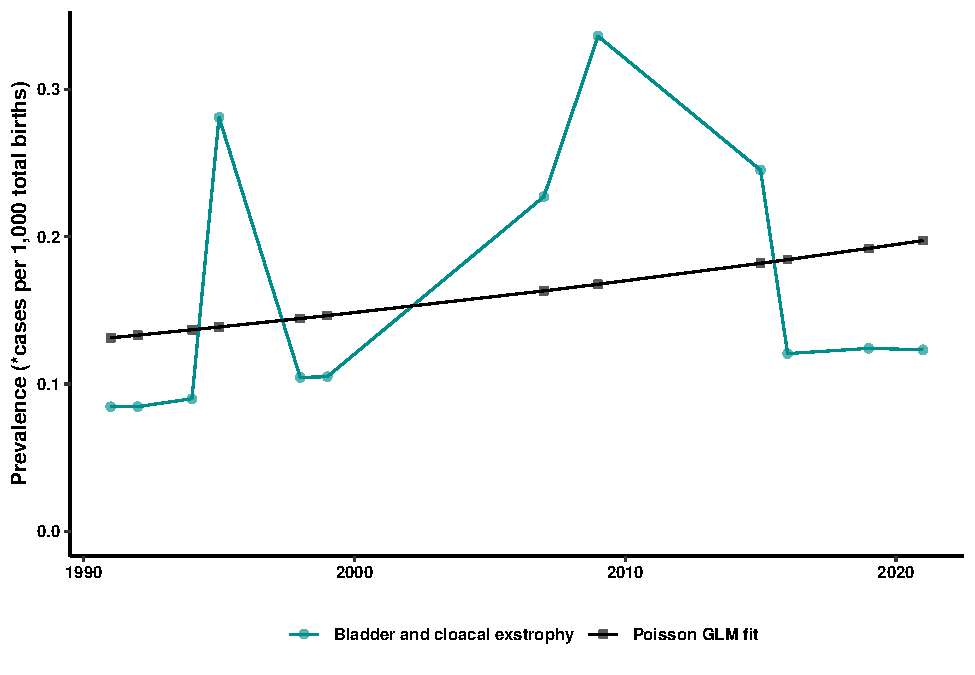
\includegraphics[width=0.65\linewidth,]{02-Trend_files/figure-latex/sutd13-1} 

}

\caption{Bladder and cloacal exstrophy - Total reported cases.}\label{fig:sutd13}
\end{figure}

\begin{itemize}
\tightlist
\item
  Lower urinary tract obstruction: there is no significant trend (\(\hat{\beta_{1}} =\) 0.01, p-value = 0.50).
\end{itemize}

\begin{figure}[h]

{\centering 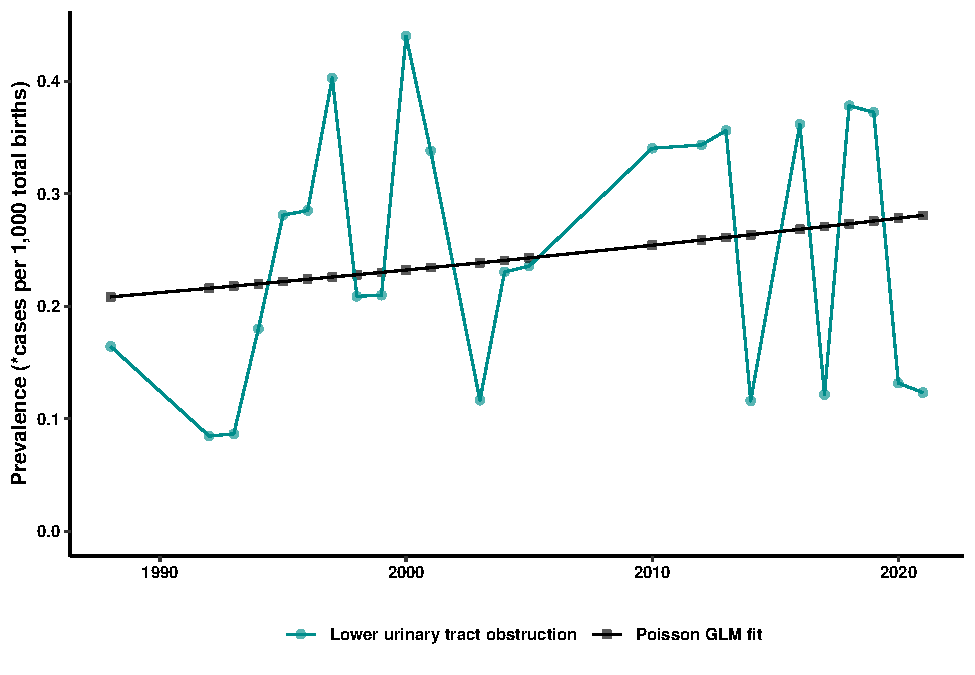
\includegraphics[width=0.65\linewidth,]{02-Trend_files/figure-latex/sutd14-1} 

}

\caption{Lower urinary tract obstruction - Total reported cases.}\label{fig:sutd14}
\end{figure}

Figure \ref{fig:sutd3} shows how the prevalence of selected urinary tract defects is geographically distributed in Nova Scotia by county between 2006 and 2020.

In the past, selected urinary tract defects appeared to be more prevalent in northern, western, and central counties. Lately, this predominance seems to have concentrated more towards the northern, western, and eastern counties, with emphasis on Shelburne, Queens, Guysborough, and Inverness counties.

\begin{figure}[h]

{\centering 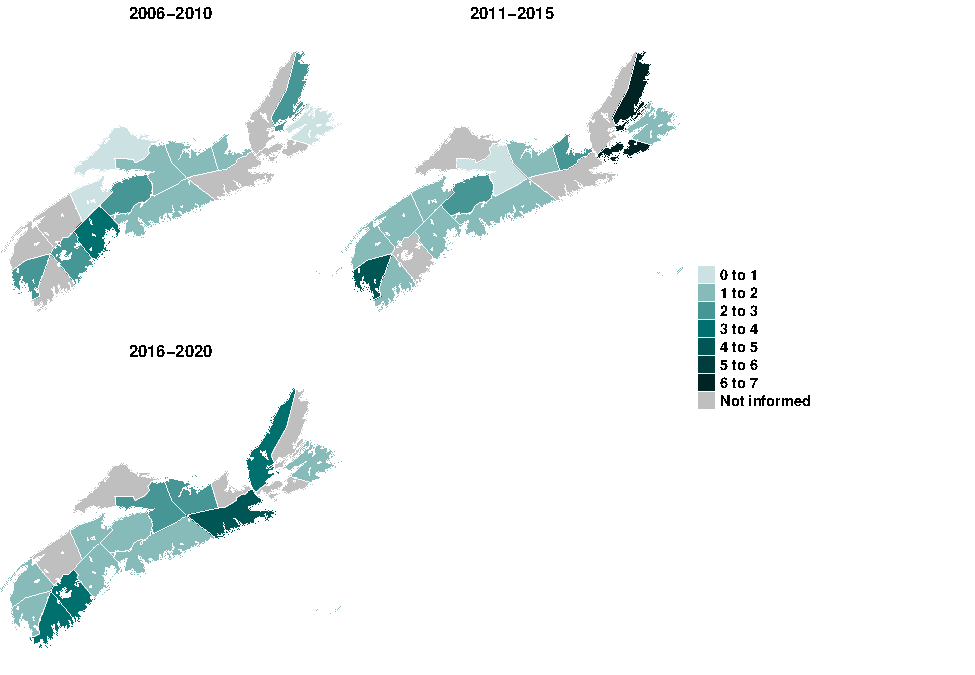
\includegraphics[width=0.65\linewidth,]{02-Trend_files/figure-latex/sutd3-1} 

}

\caption{Selected urinary tract defects - Nova Scotia. Shifts in counties between 2006 and 2020.}\label{fig:sutd3}
\end{figure}

\clearpage

\hypertarget{section310}{%
\section{Hip dysplasia}\label{section310}}

At a \(5\%\) level, there is an increasing trend for hip dysplasia (\(\hat{\beta_{1}} =\) 0.03, p-value = \textless{} 0.0001) for the period 1990 - 2021. From figure \ref{fig:hip1}, the prevalence rate exhibited steadily increased from 1990 to 2016. However, since then, there has been a significant and rapid decrease in the prevalence rate.

Over the past 10 years (2012-2021), there is evidence showing a decrease in the prevalence rate of hip dysplasia. On average, the prevalence rate for each subsequent year is 0.95 times of the previous year's rate: (prevalence rate = exp(-0.06) = 0.95 per 1,000 total births; \(\hat{\beta_{1}} =\) -0.06, p-value = \textless{} 0.0001; \(95\%\) CI for \(\hat{\beta_{1}}\) and for the prevalence rate are given by \(CI(95\%)_{\hat{\beta_{1}}}\):{[}-0.08; -0.03{]}, and \(CI(95\%)_{rate}\):{[}0.93; 0.97{]}, respectively).

\begin{figure}[h]

{\centering 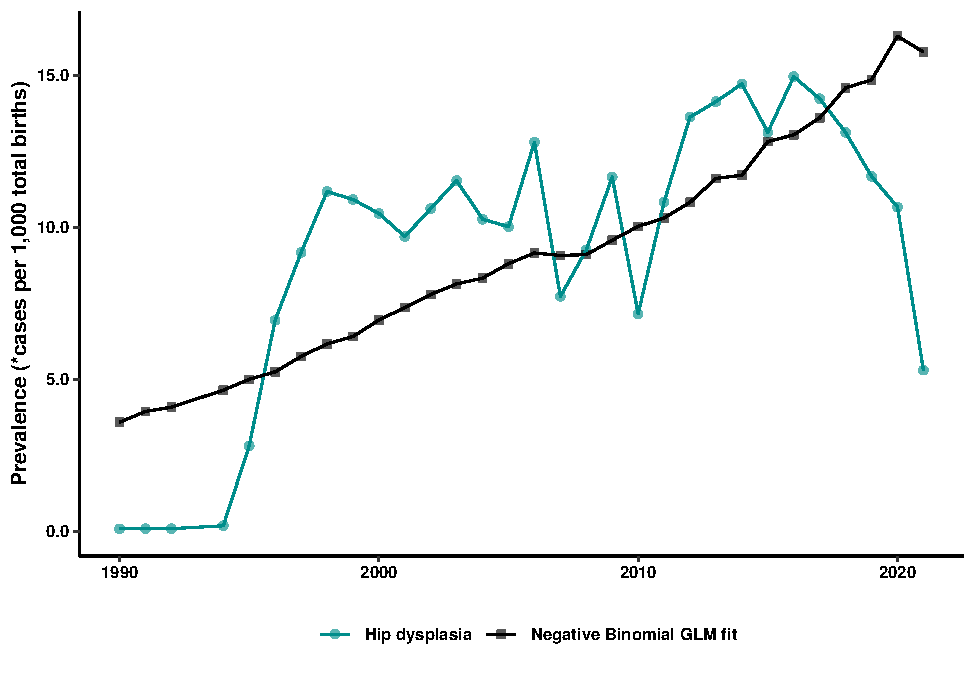
\includegraphics[width=0.65\linewidth,]{02-Trend_files/figure-latex/hip1-1} 

}

\caption{Hip dysplasia - Total reported cases.}\label{fig:hip1}
\end{figure}

Figure \ref{fig:hip3} shows how the prevalence of hip dysplasia is geographically distributed in Nova Scotia by county between 2006 and 2020.

In the past, hip dysplasia was observed throughout the province, except for Victoria county. However, in recent years, the prevalence of hip dysplasia has become more concentrated in the central, western, and eastern counties, with a higher incidence noted in Queens, Lunenburg, Hants, Halifax, and Guysborough counties.

\begin{figure}[h]

{\centering 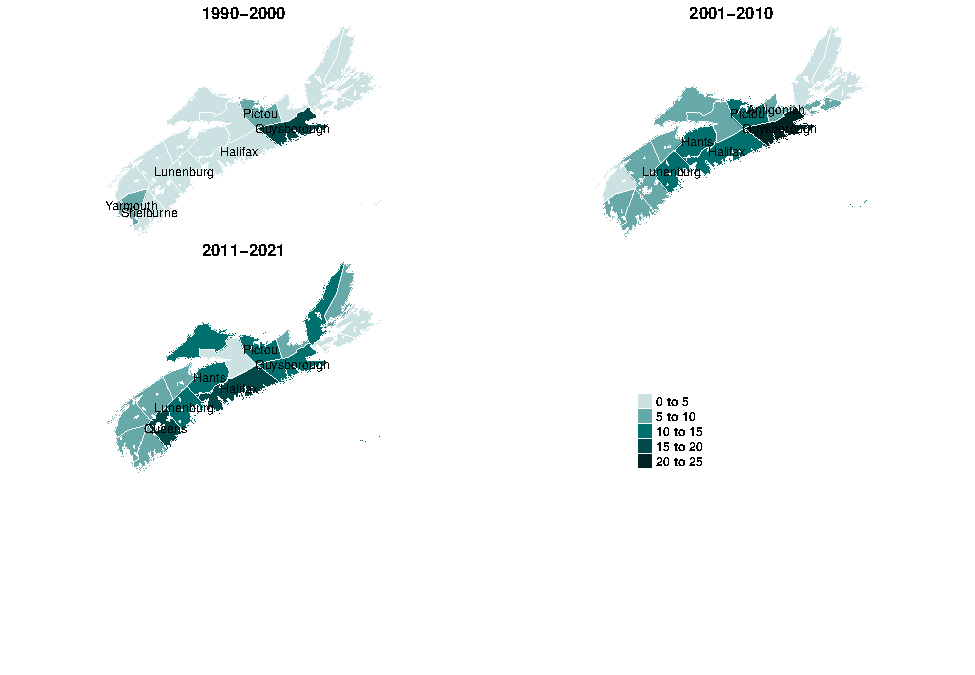
\includegraphics[width=0.65\linewidth,]{02-Trend_files/figure-latex/hip3-1} 

}

\caption{Hip dysplasia - Nova Scotia. Shifts in counties between 2006 and 2020.}\label{fig:hip3}
\end{figure}

\clearpage

\hypertarget{section311}{%
\section{Limb deficiency defects}\label{section311}}

At a \(5\%\) level, there is no significant trend for limb deficiency defects (\(\hat{\beta_{1}} =\) 0.01, p-value = 0.49) for the period 1988 - 2021. From figure \ref{fig:ldd1}, the prevalence rate exhibited an upward trend from 1988 to 2000, before returning to levels similar to those observed in 1993. Since then, the prevalence rate has fluctuated over time.

Over the past 10 years (2012-2021), there is no evidence showing any trend in the prevalence rate of limb deficiency defects. On average, the prevalence rate for each subsequent year is 0.92 times of the previous year's rate: (prevalence rate = exp(-0.09) = 0.92 per 1,000 total births; \(\hat{\beta_{1}} =\) -0.09, p-value = 0.12; \(95\%\) CI for \(\hat{\beta_{1}}\) and for the prevalence rate are given by \(CI(95\%)_{\hat{\beta_{1}}}\):{[}-0.19; 0.02{]}, and \(CI(95\%)_{rate}\):{[}0.82; 1.02{]}, respectively).

\begin{figure}[h]

{\centering 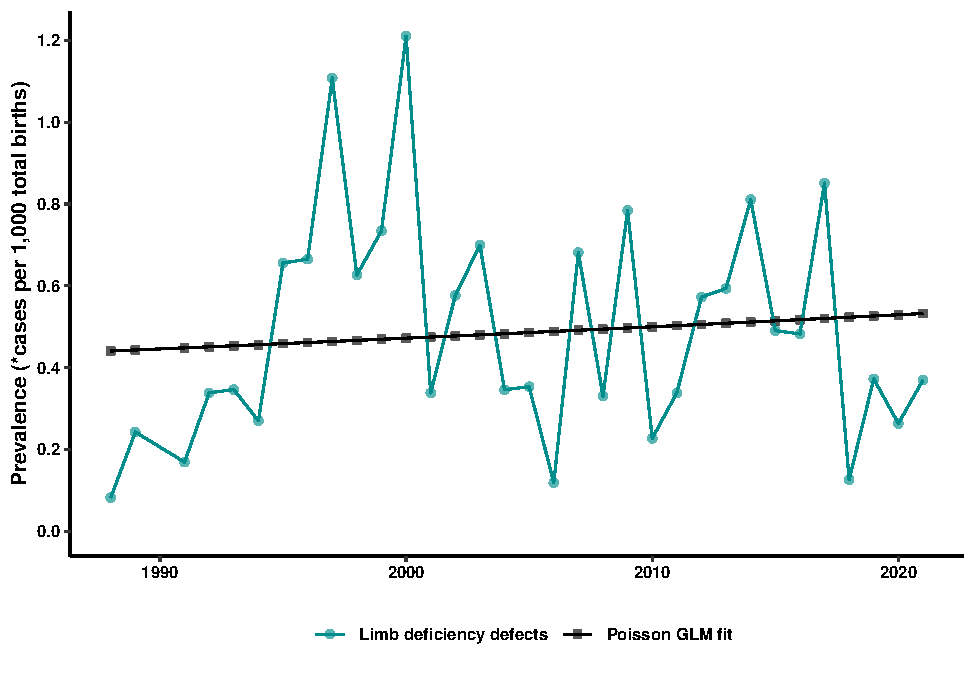
\includegraphics[width=0.65\linewidth,]{02-Trend_files/figure-latex/ldd1-1} 

}

\caption{Limb deficiency defects - Total reported cases.}\label{fig:ldd1}
\end{figure}

Figure \ref{fig:ldd3} shows how the prevalence of limb deficiency defects is geographically distributed in Nova Scotia by county between 2006 and 2020.

In the past, limb deficiency defects were more prevalent in northern counties. However, in recent years, the incidence of these defects has become more concentrated in the northern, western, and eastern counties, with a higher prevalence noted in Yarmouth, Hants, Antigonish, and Inverness counties.

\begin{figure}[h]

{\centering 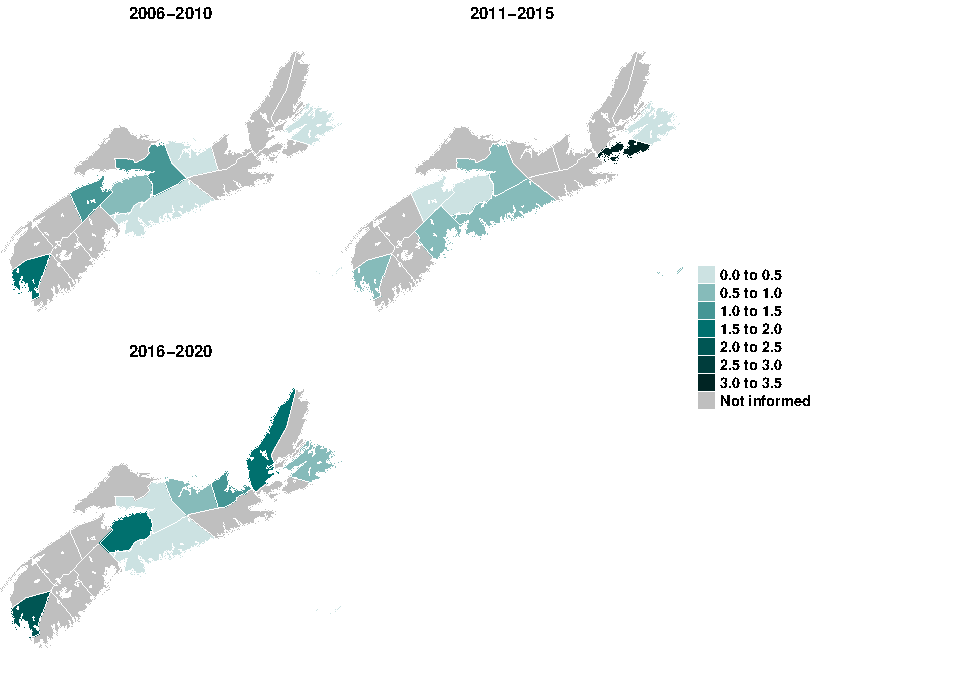
\includegraphics[width=0.65\linewidth,]{02-Trend_files/figure-latex/ldd3-1} 

}

\caption{Limb deficiency defects - Nova Scotia. Shifts in counties between 2006 and 2020.}\label{fig:ldd3}
\end{figure}

\clearpage

\hypertarget{section312}{%
\section{Selected abdominal wall defects}\label{section312}}

At a \(5\%\) level, there is no significant trend for selected abdominal wall defects (\(\hat{\beta_{1}} =\) 0.011, p-value = 0.09) for the period 1988 - 2021. From figure \ref{fig:sawd1}, the prevalence rate exhibited no clear trend and has fluctuated over time.

Over the past 10 years (2012-2021), there is no evidence showing any trend in the prevalence rate of selected abdominal wall defects. On average, the prevalence rate for each subsequent year is 1.00 times of the previous year's rate: (prevalence rate = exp(0.00) = 1.00 per 1,000 total births; \(\hat{\beta_{1}} =\) 0.00, p-value = 0.97; \(95\%\) CI for \(\hat{\beta_{1}}\) and for the prevalence rate are given by \(CI(95\%)_{\hat{\beta_{1}}}\):{[}-0.09; 0.08{]}, and \(CI(95\%)_{rate}\):{[}0.92; 1.09{]}, respectively).

\begin{figure}[h]

{\centering 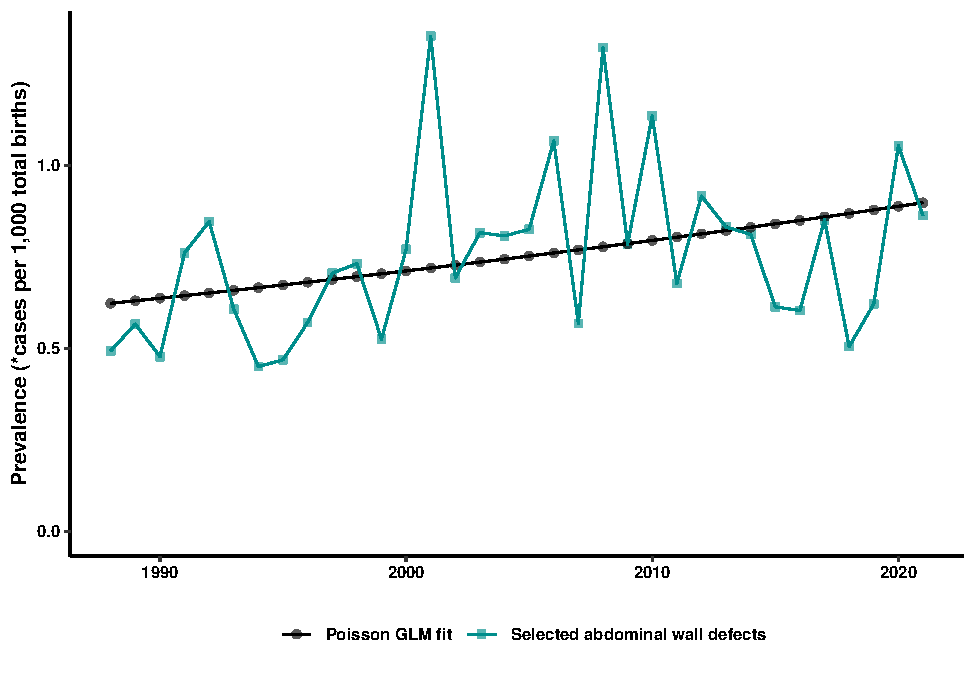
\includegraphics[width=0.65\linewidth,]{02-Trend_files/figure-latex/sawd1-1} 

}

\caption{Selected abdominal wall defects - Total reported cases.}\label{fig:sawd1}
\end{figure}

Based on the statistical analysis, at a \(5\%\) level, it is possible to observe:

\begin{itemize}
\tightlist
\item
  Diaphragmatic hernia: there is no significant trend (\(\hat{\beta_{1}} =\) -0.001, p-value = 0.89).
\end{itemize}

\begin{figure}[h]

{\centering \includegraphics[width=0.65\linewidth,]{02-Trend_files/figure-latex/sawd11-1} 

}

\caption{Diaphragmatic hernia - Total reported cases.}\label{fig:sawd11}
\end{figure}

The highest prevalence rates for diaphragmatic hernia are for mothers with maternal age \(\ge 35\).

\begin{itemize}
\tightlist
\item
  Omphalocele/Exomphalos: there is no significant trend (\(\hat{\beta_{1}} =\) -0.001, p-value = 0.96).
\end{itemize}

\begin{figure}[h]

{\centering \includegraphics[width=0.65\linewidth,]{02-Trend_files/figure-latex/sawd12-1} 

}

\caption{Omphalocele/Exomphalos - Total reported cases.}\label{fig:sawd12}
\end{figure}

The highest prevalence rates for omphalocele/exomphalos are for mothers with maternal age \(< 25\).

\begin{itemize}
\tightlist
\item
  Gastroschisis: there is evidence of an increasing trend (\(\hat{\beta_{1}} =\) 0.02, p-value = 0.05).
\end{itemize}

\begin{figure}[h]

{\centering \includegraphics[width=0.65\linewidth,]{02-Trend_files/figure-latex/sawd13-1} 

}

\caption{Gastroschisis - Total reported cases.}\label{fig:sawd13}
\end{figure}

The highest prevalence rates for gastroschisis are for mothers with maternal age \(< 25\).

Figure \ref{fig:sawd3} shows how the prevalence of selected abdominal wall defects is geographically distributed in Nova Scotia by county between 2006 and 2020.

In the past, selected abdominal wall defects appeared to be more prevalent in western, and eastern counties. Lately, this predominance seems to have remained the same, with emphasis on Yarmouth, and Inverness counties.

\begin{figure}[h]

{\centering \includegraphics[width=0.65\linewidth,]{02-Trend_files/figure-latex/sawd3-1} 

}

\caption{Selected abdominal wall defects - Nova Scotia. Shifts in counties between 2006 and 2020.}\label{fig:sawd3}
\end{figure}

\clearpage

\hypertarget{section313}{%
\section{Selected chromosomal defects}\label{section313}}

At a \(5\%\) level, there is no significant trend for selected chromosomal defects (\(\hat{\beta_{1}} =\) -0.003, p-value = 0.494) for the period 1987 - 2021. From figure \ref{fig:scd1}, the prevalence rate exhibited no clear trend and has fluctuated over time.

Over the past 10 years (2012-2021), there is evidence showing a decrease in the prevalence rate of selected chromosomal defects. On average, the prevalence rate for each subsequent year is 0.90 times of the previous year's rate: (prevalence rate = exp(-0.11) = 0.90 per 1,000 total births; \(\hat{\beta_{1}} =\) -0.11, p-value = 0.00; \(95\%\) CI for \(\hat{\beta_{1}}\) and for the prevalence rate are given by \(CI(95\%)_{\hat{\beta_{1}}}\):{[}-0.17; -0.05{]}, and \(CI(95\%)_{rate}\):{[}0.84; 0.95{]}, respectively).

\begin{figure}[h]

{\centering \includegraphics[width=0.65\linewidth,]{02-Trend_files/figure-latex/scd1-1} 

}

\caption{Selected chromosomal defects - Total reported cases.}\label{fig:scd1}
\end{figure}

Based on the statistical analysis, at a \(5\%\) level, it is possible to observe:

\begin{itemize}
\tightlist
\item
  Down Syndrome: there is no significant trend (\(\hat{\beta_{1}} =\) 0.006, p-value = 0.16).
\end{itemize}

From figure \ref{fig:scd21}, down syndrome is most commonly observed in babies born to mothers who are 35 years of age or older.

\begin{figure}[h]

{\centering \includegraphics[width=0.65\linewidth,]{02-Trend_files/figure-latex/scd21-1} 

}

\caption{Down syndrome by maternal age groups - Total reported cases.}\label{fig:scd21}
\end{figure}

\begin{itemize}
\tightlist
\item
  Trisomy 13 - Patau: there is no significant trend (\(\hat{\beta_{1}} =\) 0.050, p-value = 0.09).
\end{itemize}

From figure \ref{fig:scd22}, babies born to mothers who are 25 years of age or older have the highest risk of trisomy 13 - patau.

\begin{figure}[h]

{\centering \includegraphics[width=0.65\linewidth,]{02-Trend_files/figure-latex/scd22-1} 

}

\caption{Trisomy 13 - Patau by maternal age groups - Total reported cases.}\label{fig:scd22}
\end{figure}

\begin{itemize}
\tightlist
\item
  Trisomy 18 - Edwards: there is evidence of an increasing trend (\(\hat{\beta_{1}} =\) 0.05, p-value = 0.0001).
\end{itemize}

From figure \ref{fig:scd23}, The risk of trisomy 18 - edwards is highest in babies born to mothers who are 35 years of age or older.

\begin{figure}[h]

{\centering \includegraphics[width=0.65\linewidth,]{02-Trend_files/figure-latex/scd23-1} 

}

\caption{Trisomy 18 - Edwards by maternal age groups - Total reported cases.}\label{fig:scd23}
\end{figure}

\begin{itemize}
\tightlist
\item
  Turner syndrome: there is no significant trend (\(\hat{\beta_{1}} =\) 0.02, p-value = 0.26).
\end{itemize}

Babies born to mothers who are 25 years of age or younger have the highest risk of turner syndrome.

\begin{figure}[h]

{\centering \includegraphics[width=0.65\linewidth,]{02-Trend_files/figure-latex/scd24-1} 

}

\caption{Turner syndrome by maternal age groups - Total reported cases.}\label{fig:scd24}
\end{figure}

Figure \ref{fig:scd3} shows how the prevalence of selected chromosomal defects is geographically distributed in Nova Scotia by county between 2006 and 2020.

In the past, selected chromosomal defects appeared to be more prevalent in western, northern, and eastern counties. Lately, this predominance seems to have concentrated more towards the northern and central counties, with emphasis on Hants, and Pictou counties.

\begin{figure}[h]

{\centering \includegraphics[width=0.65\linewidth,]{02-Trend_files/figure-latex/scd3-1} 

}

\caption{Selected chromosomal defects - Nova Scotia. Shifts in counties between 2006 and 2020.}\label{fig:scd3}
\end{figure}

\hypertarget{appendix}{%
\chapter*{Appendix}\label{appendix}}


The following table of selected sentinel anomalies indicate the trends in congenital anomaly prevalence in Nova Scotia from 1987 through 2021. Sentinel anomalies are those which the International Clearinghouse of Birth Defects Surveillance and Research (ICBDSR), of which we are a member, watches worldwide with the rationale that they are quite easily identified hence more accurately reported. \emph{See Section} \ref{section21} \emph{for all the anomalies listed in the report.}

\hypertarget{section-a1}{%
\section{Appendix 1 - Linear trend analysis and p-values, 1987-2021}\label{section-a1}}

\begingroup\fontsize{7}{9}\selectfont

\begin{longtable}[t]{>{\raggedright\arraybackslash}p{4cm}cccc}
\toprule
Selected anomaly & \makecell[c]{Number of\\ periods} & \makecell[c]{Trend \\ direction} & \makecell[c]{Statistic \\ $\left(\chi^{2}_{1}\right)$} & P-value\\
\midrule
\endfirsthead
\multicolumn{5}{@{}l}{\textit{(continued)}}\\
\toprule
Selected anomaly & \makecell[c]{Number of\\ periods} & \makecell[c]{Trend \\ direction} & \makecell[c]{Statistic \\ $\left(\chi^{2}_{1}\right)$} & P-value\\
\midrule
\endhead

\endfoot
\bottomrule
\endlastfoot
Neural tube defects\newline  \tiny{ ICD-10: Q00, Q01, Q05} & \makecell[c]{34\\ \tiny{(1988-2021)}} & \makecell[c]{No significant \\ change $\left(\rightarrow \right)$} & 1.36 & 0.243\\
Anencephaly\newline  \tiny{ ICD-10: Q00} & \makecell[c]{29\\ \tiny{(1988-2020)}} & Increasing $\left(\uparrow \right)$ & 4.23 & 0.040\\
Encephalocele\newline  \tiny{ ICD-10: Q01} & \makecell[c]{22\\ \tiny{(1992-2021)}} & \makecell[c]{No significant \\ change $\left(\rightarrow \right)$} & 1.21 & 0.272\\
Spina bifida\newline  \tiny{ ICD-10: Q05} & \makecell[c]{31\\ \tiny{(1991-2021)}} & Decreasing $\left(\downarrow \right)$ & 4.03 & 0.045\\
Selected central nervous system defects\newline  \tiny{ ICD-10: Q02, Q03, Q04.1, Q04.2} & \makecell[c]{34\\ \tiny{(1988-2021)}} & Decreasing $\left(\downarrow \right)$ & 78.38 & < 0.0001\\
\addlinespace
Microcephaly\newline  \tiny{ ICD-10: Q02} & \makecell[c]{34\\ \tiny{(1988-2021)}} & Decreasing $\left(\downarrow \right)$ & 71.90 & < 0.0001\\
Congenital hydrocephalus\newline  \tiny{ ICD-10: Q03} & \makecell[c]{34\\ \tiny{(1988-2021)}} & Decreasing $\left(\downarrow \right)$ & 35.82 & < 0.0001\\
Arhinencephaly/Holoprosencephaly\newline  \tiny{ ICD-10: Q04.1, Q04.2} & \makecell[c]{14\\ \tiny{(1991-2021)}} & \makecell[c]{No significant \\ change $\left(\rightarrow \right)$} & 0.19 & 0.667\\
Selected sense organ defects\newline  \tiny{ ICD-10: Q11.0-Q11.2, Q16.0, Q17.2, Q30.0} & \makecell[c]{33\\ \tiny{(1988-2021)}} & \makecell[c]{No significant \\ change $\left(\rightarrow \right)$} & 0.13 & 0.716\\
Anophtalmos/Microphtalmos\newline  \tiny{ ICD-10: Q11.0-Q11.2} & \makecell[c]{27\\ \tiny{(1995-2021)}} & Decreasing $\left(\downarrow \right)$ & 10.78 & 0.001\\
\addlinespace
Anotia/Microtia\newline  \tiny{ ICD-10: Q16.0, Q17.2} & \makecell[c]{15\\ \tiny{(1995-2021)}} & \makecell[c]{No significant \\ change $\left(\rightarrow \right)$} & 0.99 & 0.321\\
Choanal atresia\newline  \tiny{ ICD-10: Q30.0} & \makecell[c]{32\\ \tiny{(1988-2021)}} & Decreasing $\left(\downarrow \right)$ & 6.47 & 0.011\\
Selected congenital heart defects\newline  \tiny{ ICD-10: Q20.0, Q20.1, Q20.3, Q20.5, Q21.2, Q21.3, Q23.4, Q25.1} & \makecell[c]{34\\ \tiny{(1988-2021)}} & \makecell[c]{No significant \\ change $\left(\rightarrow \right)$} & 1.52 & 0.218\\
Commom truncus\newline  \tiny{ ICD-10: Q20.0} & \makecell[c]{21\\ \tiny{(1991-2021)}} & Decreasing $\left(\downarrow \right)$ & 5.25 & 0.022\\
Transposition of great vessels\newline  \tiny{ ICD-10: Other} & \makecell[c]{34\\ \tiny{(1988-2021)}} & Decreasing $\left(\downarrow \right)$ & 6.02 & 0.014\\
\addlinespace
Atrioventricular septal defect\newline  \tiny{ ICD-10: Q21.2} & \makecell[c]{34\\ \tiny{(1988-2021)}} & \makecell[c]{No significant \\ change $\left(\rightarrow \right)$} & 0.25 & 0.620\\
Tetralogy of Fallot\newline  \tiny{ ICD-10: Q21.3} & \makecell[c]{34\\ \tiny{(1988-2021)}} & \makecell[c]{No significant \\ change $\left(\rightarrow \right)$} & 1.60 & 0.206\\
Hypoplastic left heart syndrome\newline  \tiny{ ICD-10: Q23.4} & \makecell[c]{34\\ \tiny{(1988-2021)}} & \makecell[c]{No significant \\ change $\left(\rightarrow \right)$} & 1.10 & 0.295\\
Coarctation of aorta\newline  \tiny{ ICD-10: Q25.1} & \makecell[c]{34\\ \tiny{(1988-2021)}} & \makecell[c]{No significant \\ change $\left(\rightarrow \right)$} & 0.25 & 0.615\\
Oro-facial clefts\newline  \tiny{ ICD-10: Q35-Q37, excludes Q35.7} & \makecell[c]{34\\ \tiny{(1988-2021)}} & \makecell[c]{No significant \\ change $\left(\rightarrow \right)$} & 0.20 & 0.654\\
\addlinespace
Cleft palate only\newline  \tiny{ ICD-10: Other} & \makecell[c]{34\\ \tiny{(1988-2021)}} & \makecell[c]{No significant \\ change $\left(\rightarrow \right)$} & 0.19 & 0.661\\
Cleft lip only\newline  \tiny{ ICD-10: Other} & \makecell[c]{26\\ \tiny{(1988-2020)}} & \makecell[c]{No significant \\ change $\left(\rightarrow \right)$} & 3.24 & 0.072\\
Cleft palate with cleft lip\newline  \tiny{ ICD-10: Q37} & \makecell[c]{34\\ \tiny{(1988-2021)}} & \makecell[c]{No significant \\ change $\left(\rightarrow \right)$} & 0.11 & 0.740\\
Selected gastrointestinal defects\newline  \tiny{ ICD-10: Q39.0-Q39.4, Q41, Q42.0-Q42.3, Q43.1, Q44.2} & \makecell[c]{34\\ \tiny{(1988-2021)}} & Increasing $\left(\uparrow \right)$ & 10.30 & 0.001\\
Oesophageal atresia/stenosis, tracheoesophageal fistula\newline  \tiny{ ICD-10: Q39.0-Q39.4} & \makecell[c]{32\\ \tiny{(1988-2021)}} & \makecell[c]{No significant \\ change $\left(\rightarrow \right)$} & 2.53 & 0.112\\
\addlinespace
Small intestine absence/atresia/stenosis\newline  \tiny{ ICD-10: Q41} & \makecell[c]{30\\ \tiny{(1992-2021)}} & \makecell[c]{No significant \\ change $\left(\rightarrow \right)$} & 0.40 & 0.525\\
Ano-rectal absence/atresia/stenosis\newline  \tiny{ ICD-10: Q42.0-Q42.3} & \makecell[c]{24\\ \tiny{(1992-2021)}} & Increasing $\left(\uparrow \right)$ & 8.00 & 0.005\\
Hirschsprung disease\newline  \tiny{ ICD-10: Q43.1} & \makecell[c]{31\\ \tiny{(1988-2021)}} & \makecell[c]{No significant \\ change $\left(\rightarrow \right)$} & 1.13 & 0.288\\
Atresia of bile ducts\newline  \tiny{ ICD-10: Q44.2} & \makecell[c]{21\\ \tiny{(1994-2021)}} & \makecell[c]{No significant \\ change $\left(\rightarrow \right)$} & 0.63 & 0.428\\
Selected genital anomalies\newline  \tiny{ ICD-10: Q53.1, Q53.2, Q53.9, Q54, excludes Q54.4, Q56, Q64.0} & \makecell[c]{34\\ \tiny{(1988-2021)}} & Increasing $\left(\uparrow \right)$ & 4.53 & 0.033\\
\addlinespace
Cryptorchidism/undescended testicles\newline  \tiny{ ICD-10: Q53.1, Q53.2, Q53.9} & \makecell[c]{34\\ \tiny{(1988-2021)}} & Decreasing $\left(\downarrow \right)$ & 47.02 & < 0.0001\\
Hypospadias\newline  \tiny{ ICD-10: Q54, excludes Q54.4} & \makecell[c]{27\\ \tiny{(1993-2021)}} & Increasing $\left(\uparrow \right)$ & 118.78 & < 0.0001\\
Indeterminate sex\newline  \tiny{ ICD-10: Q56} & \makecell[c]{25\\ \tiny{(1988-2021)}} & \makecell[c]{No significant \\ change $\left(\rightarrow \right)$} & 0.40 & 0.528\\
Epispadias\newline  \tiny{ ICD-10: Q64.0} & \makecell[c]{24\\ \tiny{(1988-2021)}} & \makecell[c]{No significant \\ change $\left(\rightarrow \right)$} & 0.24 & 0.622\\
Selected urinary tract defects\newline  \tiny{ ICD-10: Q60.0-Q60.2, Q61.1-Q61.5, Q61.8, Q61.9, Q64.1-Q64.3} & \makecell[c]{34\\ \tiny{(1988-2021)}} & Increasing $\left(\uparrow \right)$ & 18.19 & < 0.0001\\
\addlinespace
Renal agenesis\newline  \tiny{ ICD-10: Q60.0-Q60.2} & \makecell[c]{29\\ \tiny{(1992-2021)}} & Increasing $\left(\uparrow \right)$ & 4.51 & 0.034\\
Cystic kidney\newline  \tiny{ ICD-10: Q61.1-Q61.5, Q61.8, Q61.9} & \makecell[c]{34\\ \tiny{(1988-2021)}} & \makecell[c]{No significant \\ change $\left(\rightarrow \right)$} & 1.13 & 0.288\\
Bladder and cloacal exstrophy\newline  \tiny{ ICD-10: Q64.1} & \makecell[c]{12\\ \tiny{(1991-2021)}} & \makecell[c]{No significant \\ change $\left(\rightarrow \right)$} & 0.39 & 0.534\\
Lower urinary tract obstruction\newline  \tiny{ ICD-10: Q64.2, Q64.3} & \makecell[c]{24\\ \tiny{(1988-2021)}} & \makecell[c]{No significant \\ change $\left(\rightarrow \right)$} & 0.46 & 0.498\\
Hip dysplasia\newline  \tiny{ ICD-10: Q65} & \makecell[c]{31\\ \tiny{(1990-2021)}} & Increasing $\left(\uparrow \right)$ & 490.87 & < 0.0001\\
\addlinespace
Limb deficiency defects\newline  \tiny{ ICD-10: Q71-Q73} & \makecell[c]{33\\ \tiny{(1988-2021)}} & \makecell[c]{No significant \\ change $\left(\rightarrow \right)$} & 0.47 & 0.493\\
Selected abdominal wall defects\newline  \tiny{ ICD-10: Q79.2, Q79.3} & \makecell[c]{34\\ \tiny{(1988-2021)}} & \makecell[c]{No significant \\ change $\left(\rightarrow \right)$} & 2.92 & 0.087\\
Omphalocele/Exomphalos\newline  \tiny{ ICD-10: Q79.2} & \makecell[c]{25\\ \tiny{(1992-2021)}} & \makecell[c]{No significant \\ change $\left(\rightarrow \right)$} & 0.00 & 0.958\\
Gastroschisis\newline  \tiny{ ICD-10: Q79.3} & \makecell[c]{34\\ \tiny{(1988-2021)}} & Increasing $\left(\uparrow \right)$ & 3.89 & 0.049\\
Selected chromosomal defects\newline  \tiny{ ICD-10: Q90, Q91.0-Q91.7, Q96} & \makecell[c]{35\\ \tiny{(1987-2021)}} & \makecell[c]{No significant \\ change $\left(\rightarrow \right)$} & 0.47 & 0.494\\
\addlinespace
Down Syndrome\newline  \tiny{ ICD-10: Q90} & \makecell[c]{35\\ \tiny{(1987-2021)}} & \makecell[c]{No significant \\ change $\left(\rightarrow \right)$} & 1.97 & 0.161\\
Trisomy 13 - Patau\newline  \tiny{ ICD-10: Q91.4-Q91.7} & \makecell[c]{11\\ \tiny{(1994-2018)}} & \makecell[c]{No significant \\ change $\left(\rightarrow \right)$} & 2.81 & 0.094\\
Trisomy 18 - Edwards\newline  \tiny{ ICD-10: Q91.0-Q91.3} & \makecell[c]{27\\ \tiny{(1988-2019)}} & Increasing $\left(\uparrow \right)$ & 14.71 & < 0.0001\\
Turner syndrome\newline  \tiny{ ICD-10: Q96} & \makecell[c]{22\\ \tiny{(1989-2021)}} & \makecell[c]{No significant \\ change $\left(\rightarrow \right)$} & 1.25 & 0.263\\*
\end{longtable}
\endgroup{}

\clearpage

\hypertarget{section-a2}{%
\section{Appendix 2 - Total birth, number of cases, anomalies and anomalies per case, 1987-2021}\label{section-a2}}

\begingroup\fontsize{7}{9}\selectfont

\begin{longtable}[t]{cccccc}
\toprule
Year & \makecell[c]{Number of \\ cases} & \makecell[c]{Number of \\ anomalies} & \makecell[c]{Case \\ rate} & \makecell[c]{Anomaly \\ rate} & \makecell[c]{Anomaly rate \\ per case}\\
\midrule
\endfirsthead
\multicolumn{6}{@{}l}{\textit{(continued)}}\\
\toprule
Year & \makecell[c]{Number of \\ cases} & \makecell[c]{Number of \\ anomalies} & \makecell[c]{Case \\ rate} & \makecell[c]{Anomaly \\ rate} & \makecell[c]{Anomaly rate \\ per case}\\
\midrule
\endhead

\endfoot
\bottomrule
\endlastfoot
\cellcolor{gray!6}{1987} & \cellcolor{gray!6}{7} & \cellcolor{gray!6}{10} & \cellcolor{gray!6}{52.24} & \cellcolor{gray!6}{74.63} & \cellcolor{gray!6}{1.43}\\
1988 & 802 & 900 & 65.87 & 73.92 & 1.12\\
\cellcolor{gray!6}{1989} & \cellcolor{gray!6}{735} & \cellcolor{gray!6}{833} & \cellcolor{gray!6}{59.44} & \cellcolor{gray!6}{67.36} & \cellcolor{gray!6}{1.13}\\
1990 & 854 & 980 & 67.87 & 77.89 & 1.15\\
\cellcolor{gray!6}{1991} & \cellcolor{gray!6}{872} & \cellcolor{gray!6}{995} & \cellcolor{gray!6}{73.69} & \cellcolor{gray!6}{84.08} & \cellcolor{gray!6}{1.14}\\
\addlinespace
1992 & 892 & 1,054 & 75.45 & 89.16 & 1.18\\
\cellcolor{gray!6}{1993} & \cellcolor{gray!6}{905} & \cellcolor{gray!6}{1,050} & \cellcolor{gray!6}{78.38} & \cellcolor{gray!6}{90.93} & \cellcolor{gray!6}{1.16}\\
1994 & 849 & 1,024 & 76.38 & 92.13 & 1.21\\
\cellcolor{gray!6}{1995} & \cellcolor{gray!6}{1,002} & \cellcolor{gray!6}{1,257} & \cellcolor{gray!6}{93.84} & \cellcolor{gray!6}{117.72} & \cellcolor{gray!6}{1.25}\\
1996 & 1,291 & 1,727 & 122.71 & 164.15 & 1.34\\
\addlinespace
\cellcolor{gray!6}{1997} & \cellcolor{gray!6}{1,379} & \cellcolor{gray!6}{1,810} & \cellcolor{gray!6}{138.89} & \cellcolor{gray!6}{182.29} & \cellcolor{gray!6}{1.31}\\
1998 & 1,416 & 1,949 & 147.85 & 203.51 & 1.38\\
\cellcolor{gray!6}{1999} & \cellcolor{gray!6}{1,536} & \cellcolor{gray!6}{1,936} & \cellcolor{gray!6}{161.16} & \cellcolor{gray!6}{203.13} & \cellcolor{gray!6}{1.26}\\
2000 & 1,604 & 2,010 & 176.48 & 221.15 & 1.25\\
\cellcolor{gray!6}{2001} & \cellcolor{gray!6}{1,605} & \cellcolor{gray!6}{2,062} & \cellcolor{gray!6}{180.89} & \cellcolor{gray!6}{232.39} & \cellcolor{gray!6}{1.28}\\
\addlinespace
2002 & 1,444 & 1,930 & 166.55 & 222.61 & 1.34\\
\cellcolor{gray!6}{2003} & \cellcolor{gray!6}{1,151} & \cellcolor{gray!6}{1,746} & \cellcolor{gray!6}{134.10} & \cellcolor{gray!6}{203.43} & \cellcolor{gray!6}{1.52}\\
2004 & 1,012 & 1,633 & 116.66 & 188.24 & 1.61\\
\cellcolor{gray!6}{2005} & \cellcolor{gray!6}{996} & \cellcolor{gray!6}{1,569} & \cellcolor{gray!6}{117.36} & \cellcolor{gray!6}{184.87} & \cellcolor{gray!6}{1.58}\\
2006 & 1,143 & 1,765 & 135.43 & 209.12 & 1.54\\
\addlinespace
\cellcolor{gray!6}{2007} & \cellcolor{gray!6}{1,113} & \cellcolor{gray!6}{1,778} & \cellcolor{gray!6}{126.41} & \cellcolor{gray!6}{201.93} & \cellcolor{gray!6}{1.60}\\
2008 & 1,232 & 1,986 & 135.68 & 218.72 & 1.61\\
\cellcolor{gray!6}{2009} & \cellcolor{gray!6}{1,236} & \cellcolor{gray!6}{2,033} & \cellcolor{gray!6}{138.46} & \cellcolor{gray!6}{227.74} & \cellcolor{gray!6}{1.64}\\
2010 & 1,215 & 2,006 & 137.88 & 227.64 & 1.65\\
\cellcolor{gray!6}{2011} & \cellcolor{gray!6}{1,272} & \cellcolor{gray!6}{2,103} & \cellcolor{gray!6}{143.45} & \cellcolor{gray!6}{237.17} & \cellcolor{gray!6}{1.65}\\
\addlinespace
2012 & 1,201 & 1,956 & 137.48 & 223.90 & 1.63\\
\cellcolor{gray!6}{2013} & \cellcolor{gray!6}{1,417} & \cellcolor{gray!6}{2,270} & \cellcolor{gray!6}{168.23} & \cellcolor{gray!6}{269.50} & \cellcolor{gray!6}{1.60}\\
2014 & 1,874 & 3,236 & 217.07 & 374.84 & 1.73\\
\cellcolor{gray!6}{2015} & \cellcolor{gray!6}{1,529} & \cellcolor{gray!6}{2,220} & \cellcolor{gray!6}{187.47} & \cellcolor{gray!6}{272.19} & \cellcolor{gray!6}{1.45}\\
2016 & 1,345 & 1,915 & 162.18 & 230.92 & 1.42\\
\addlinespace
\cellcolor{gray!6}{2017} & \cellcolor{gray!6}{1,289} & \cellcolor{gray!6}{1,758} & \cellcolor{gray!6}{156.72} & \cellcolor{gray!6}{213.74} & \cellcolor{gray!6}{1.36}\\
2018 & 1,390 & 1,912 & 175.28 & 241.11 & 1.38\\
\cellcolor{gray!6}{2019} & \cellcolor{gray!6}{1,442} & \cellcolor{gray!6}{2,011} & \cellcolor{gray!6}{179.02} & \cellcolor{gray!6}{249.66} & \cellcolor{gray!6}{1.39}\\
2020 & 1,282 & 1,754 & 168.77 & 230.91 & 1.37\\
\cellcolor{gray!6}{2021} & \cellcolor{gray!6}{1,378} & \cellcolor{gray!6}{1,908} & \cellcolor{gray!6}{169.79} & \cellcolor{gray!6}{235.09} & \cellcolor{gray!6}{1.38}\\*
\end{longtable}
\endgroup{}


\end{document}
